% ============================================================
%  CHƯƠNG 3: THỰC NGHIỆM
% ============================================================

\chapter{Thực nghiệm và đánh giá}
\label{chap:thuc-nghiem}

Chương này trình bày kết quả thực nghiệm Thuật toán~\ref{alg:spectral-clustering} với đầu vào $W = W_\lambda = A + \lambda W^{(M)}$ ($M = K_3$) trên hai loại dữ liệu. Loại thứ nhất gồm bốn mô hình sinh ngẫu nhiên có cấu trúc cộng đồng (SBM, Planted Partition, GRPG, LFR). Loại thứ hai gồm mười đồ thị mạng xã hội thật. Định nghĩa hình thức của các mô hình sinh ngẫu nhiên xem Phụ lục~\ref{appx:random-models}.

% ============================================================
\section{Thiết lập thí nghiệm}
\label{sec:setup}

\textbf{Quét tham số.} $\lambda \in \{0,\ 0.5,\ 1,\ 2,\ 5,\ 10\}$ kèm trường hợp $W_M$ thuần (tương ứng $\lambda \to \infty$). Trường hợp $\lambda = 0$ trùng với phân cụm phổ cổ điển trên ma trận kề $A$ và được dùng làm chuẩn so sánh.

\textbf{Số cụm $K$.} Với đồ thị có phân hoạch chuẩn, đặt $K = K_{\mathrm{gt}}$ là số cộng đồng thật. Với đồ thị mạng xã hội không có phân hoạch chuẩn, quét $K \in \{50, 100, 200, 300, 400, 500\}$ cho mỗi đồ thị.

\textbf{Chỉ số đánh giá.} Mọi chỉ số được tính trên đồ thị gốc $A$, không phải trên $W_\lambda$:
\begin{itemize}
    \item Modularity $Q$ là chỉ số chất lượng chính.
    \item NMI và Jaccard so với phân hoạch chuẩn (khi có).
    \item $\overline{\mathrm{CC}}$, $\overline{\mathrm{CC}}_w$: hệ số phân cụm tổng hợp.
    \item Số cạnh bị cắt và số motif (tam giác) bị cắt qua biên cụm.
\end{itemize}

\textbf{Mục tiêu.} Với mỗi bộ test, ghi lại $Q(\lambda)$ cho từng giá trị $\lambda$. Đặt
\[
    \Delta Q = \max_{\lambda > 0} Q(\lambda) - Q(0)
\]
là mức tăng tốt nhất do ma trận hỗn hợp đem lại so với phân cụm phổ cổ điển. $\Delta Q > 0$ chứng tỏ $W_\lambda$ với $\lambda > 0$ phù hợp hơn $A$; $\lambda^*$ đạt cực đại là giá trị tối ưu cho bộ test.

% ============================================================
\section{Đồ thị có cấu trúc cộng đồng}
\label{sec:results-synthetic}

Bảng~\ref{tab:synthetic-summary} tổng hợp kết quả tốt nhất trên bốn mô hình. Với mỗi mô hình, năm bộ test có $\Delta Q$ lớn nhất (lọc $Q(0) \geq 0{,}1$ để tránh phân hoạch tầm thường) được chọn.

\begin{table}[H]
\centering
\caption{Kết quả tốt nhất trên bốn mô hình có cấu trúc cộng đồng}
\label{tab:synthetic-summary}
\begin{tabular}{|l|l|c|c|c|c|}
\hline
\textbf{Mô hình} & \textbf{Bộ test tốt nhất} & $Q(0)$ & $\lambda^*$ & $Q(\lambda^*)$ & $\Delta Q$ \\ \hline
LFR     & LFR-100-$\mu{=}0{,}35$       & 0{,}1124 & 5{,}0    & 0{,}4785 & $+0{,}3661$ \\ \hline
GRPG    & GRPG-2000-$p_{\mathrm{out}}{=}0{,}006$ & 0{,}1165 & 1{,}0 & 0{,}2005 & $+0{,}0840$ \\ \hline
Planted & Planted-$k{=}5$-$p_{\mathrm{out}}{=}0{,}025$ & 0{,}1203 & 0{,}5 & 0{,}2185 & $+0{,}0982$ \\ \hline
SBM     & SBM-1500-$p_{\mathrm{out}}{=}0{,}008$ & 0{,}1673 & 0{,}5 & 0{,}1975 & $+0{,}0302$ \\ \hline
\end{tabular}
\end{table}

% ............................................................
\subsection{LFR Benchmark}
\label{subsec:results-lfr}

Bộ dữ liệu Lancichinetti--Fortunato--Radicchi (LFR) được công nhận rộng rãi như benchmark chuẩn cho bài toán phát hiện cộng đồng nhờ phân bố bậc và phân bố kích thước cụm cùng tuân theo luỹ thừa, gần với cấu trúc của nhiều mạng thật. Tham số then chốt là mixing parameter $\mu \in (0, 1)$: mỗi đỉnh dành tỉ lệ $1 - \mu$ số cạnh cho cộng đồng của mình và tỉ lệ $\mu$ số cạnh cho phần còn lại của đồ thị. Giá trị $\mu$ càng lớn, ranh giới cộng đồng càng mờ và bài toán càng khó. Khoá luận quét $n \in \{100, 500, 2000\}$ và $\mu \in \{0{,}2,\ 0{,}35,\ 0{,}4,\ 0{,}5\}$, các tham số còn lại giữ mặc định của thuật toán sinh.

\subsubsection*{Modularity và NMI}

Bảng~\ref{tab:lfr-top5} trình bày năm bộ test LFR có $\Delta Q$ lớn nhất. Hình~\ref{fig:lfr-modularity} và Hình~\ref{fig:lfr-nmi} lần lượt cho biểu đồ modularity và NMI theo $\lambda$.

\begin{table}[H]
\centering
\caption{Năm bộ test LFR có cải thiện modularity lớn nhất}
\label{tab:lfr-top5}
\begin{tabular}{|l|c|c|c|c|c|c|}
\hline
\textbf{Bộ test} & $Q(0)$ & $\lambda{=}0{,}5$ & $\lambda{=}1$ & $\lambda{=}2$ & $\lambda{=}5$ & $\lambda^*$ \\ \hline
LFR-100-$\mu0{,}35$  & 0{,}1124 & 0{,}0042 & 0{,}0838 & 0{,}2942 & \textbf{0{,}4785} & $5{,}0$ \\ \hline
LFR-100-$\mu0{,}2$   & 0{,}4747 & 0{,}4858 & 0{,}4761 & \textbf{0{,}6280} & 0{,}6255 & $2{,}0$ \\ \hline
LFR-500-$\mu0{,}4$   & 0{,}1670 & \textbf{0{,}2979} & 0{,}2951 & 0{,}2778 & 0{,}2708 & $0{,}5$ \\ \hline
LFR-2000-$\mu0{,}5$  & 0{,}1112 & 0{,}2348 & \textbf{0{,}2409} & 0{,}2382 & 0{,}2275 & $1{,}0$ \\ \hline
LFR-500-$\mu0{,}35$  & 0{,}2181 & \textbf{0{,}3380} & 0{,}2992 & 0{,}3270 & 0{,}3199 & $0{,}5$ \\ \hline
\end{tabular}
\end{table}

\begin{figure}[H]
    \centering
    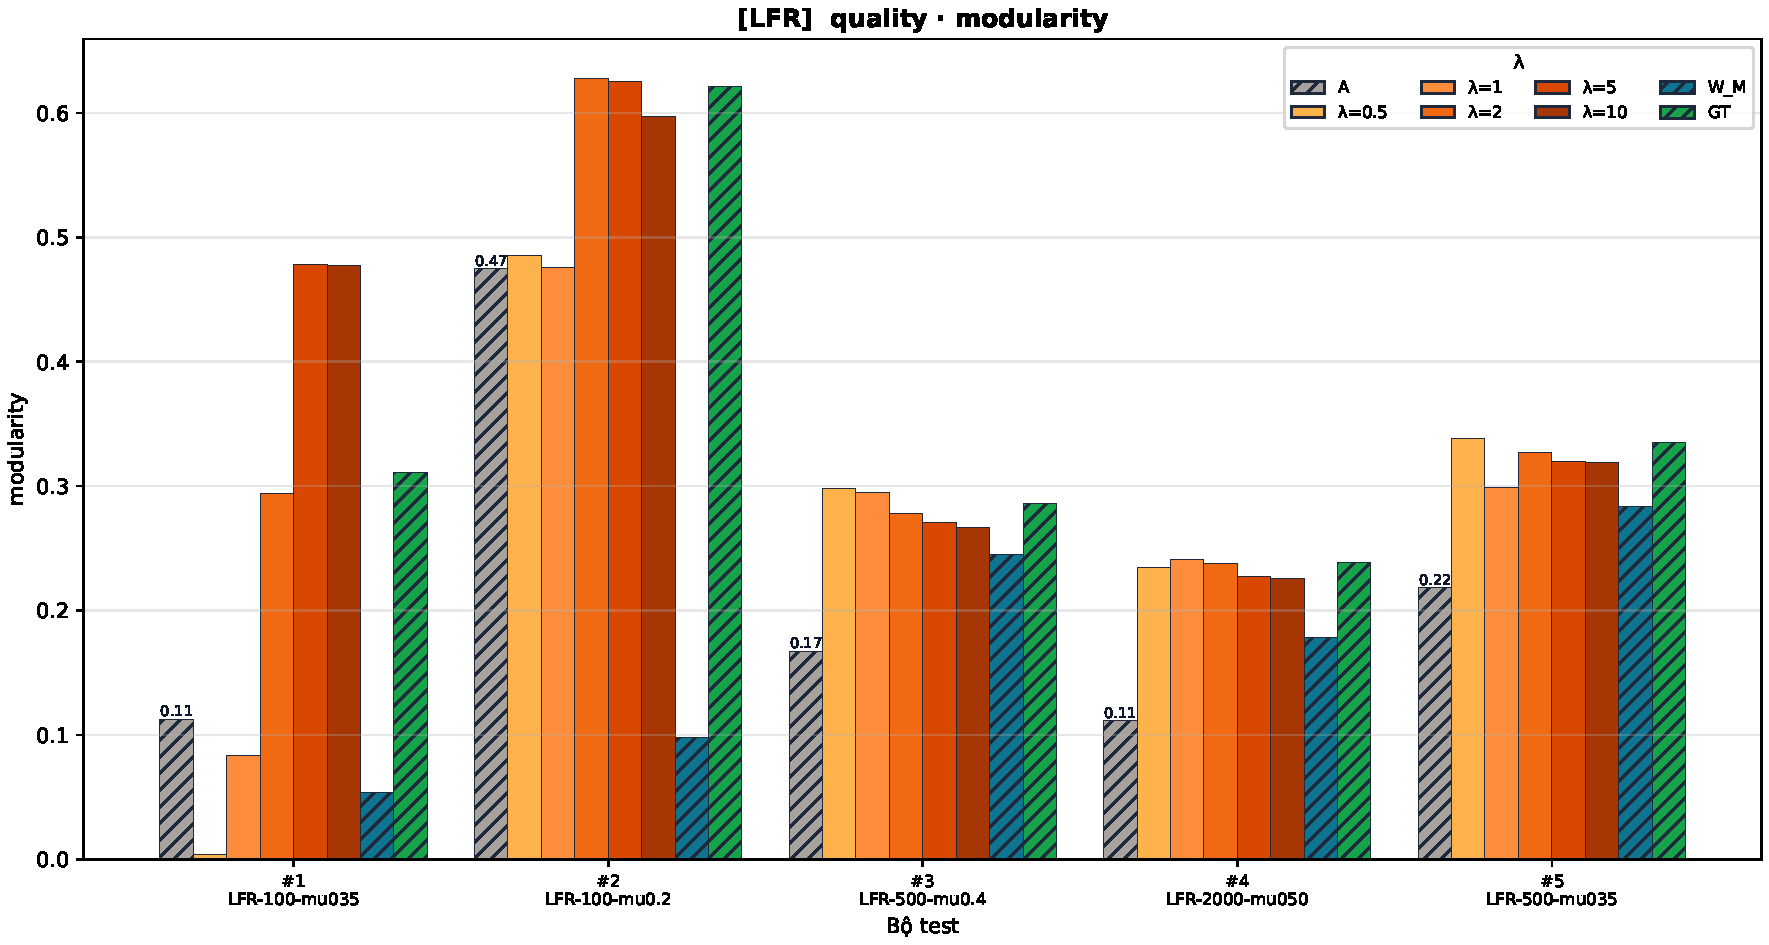
\includegraphics[width=\textwidth]{../main_result/LFR/charts/quality_modularity.pdf}
    \caption[Modularity $Q$ trên năm bộ LFR theo $\lambda$.]{Modularity $Q$ trên năm bộ LFR có $\Delta Q$ lớn nhất theo $\lambda$.}
    \label{fig:lfr-modularity}
\end{figure}

\begin{figure}[H]
    \centering
    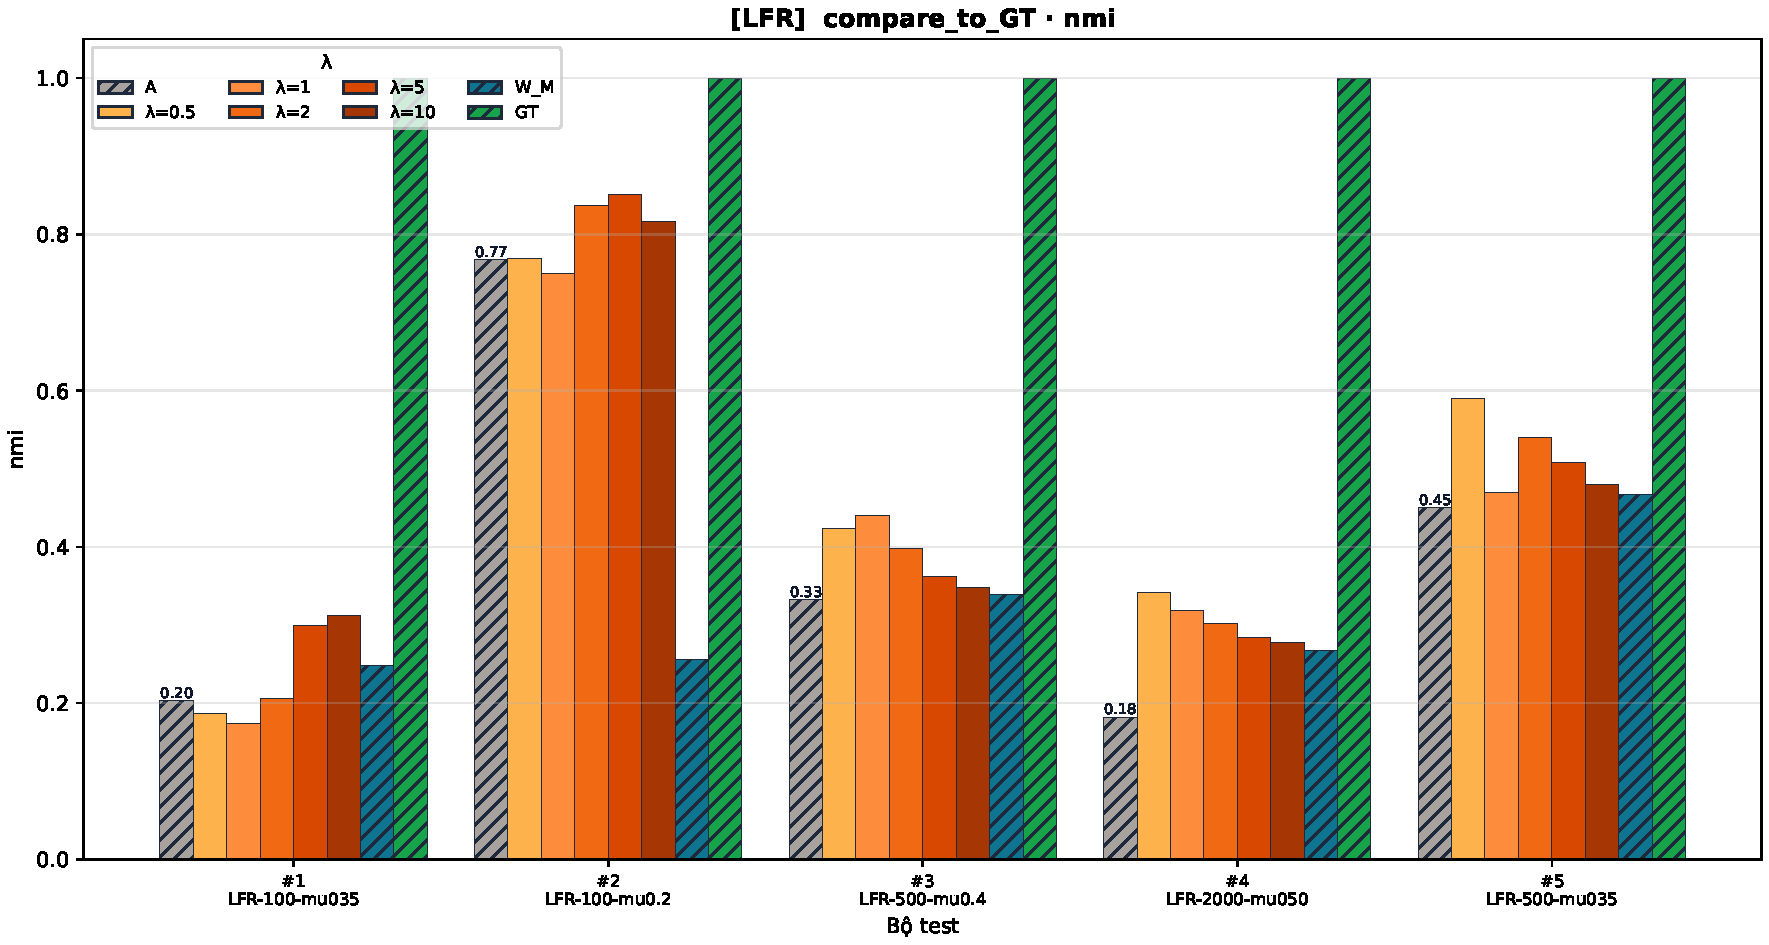
\includegraphics[width=\textwidth]{../main_result/LFR/charts/compare_to_GT_nmi.pdf}
    \caption{NMI so với phân hoạch chuẩn trên năm bộ LFR theo $\lambda$.}
    \label{fig:lfr-nmi}
\end{figure}

\textbf{Quan sát.} $Q$ tăng trên toàn dải $\mu$, biên độ lớn nhất tập trung ở vùng cộng đồng tách yếu. Bộ LFR-100-$\mu0{,}35$ minh hoạ rõ nhất khi $Q$ chuyển từ $0{,}1124$ tại $\lambda = 0$ lên $0{,}4785$ tại $\lambda = 5$, và NMI đồng pha tăng từ $0{,}2026$ lên $0{,}3124$. Giá trị $\lambda^*$ tối ưu phân tán trong khoảng $0{,}5$ đến $5$ tuỳ bộ test.

\textbf{Nhận xét.} Mức cải thiện chỉ rõ rệt khi modularity ban đầu thấp. Khi $\mu$ nhỏ, các cạnh nội cụm đã đủ rõ để phân cụm phổ trên $A$ hoạt động tốt, đóng góp của motif bị bão hoà. Sự đồng pha của $Q$ và NMI là yếu tố then chốt: phân hoạch thu được không chỉ tối ưu theo chỉ số nội tại mà còn gần phân hoạch chuẩn hơn, loại trừ khả năng modularity tăng do thuật toán bị đẩy về một phân hoạch tốt giả tạo. Phân tán của $\lambda^*$ cho thấy cần chiến lược chọn $\lambda$ phụ thuộc đồ thị, không tồn tại quy tắc cố định toàn cục.

\subsubsection*{Hệ số phân cụm}

\begin{figure}[H]
    \centering
    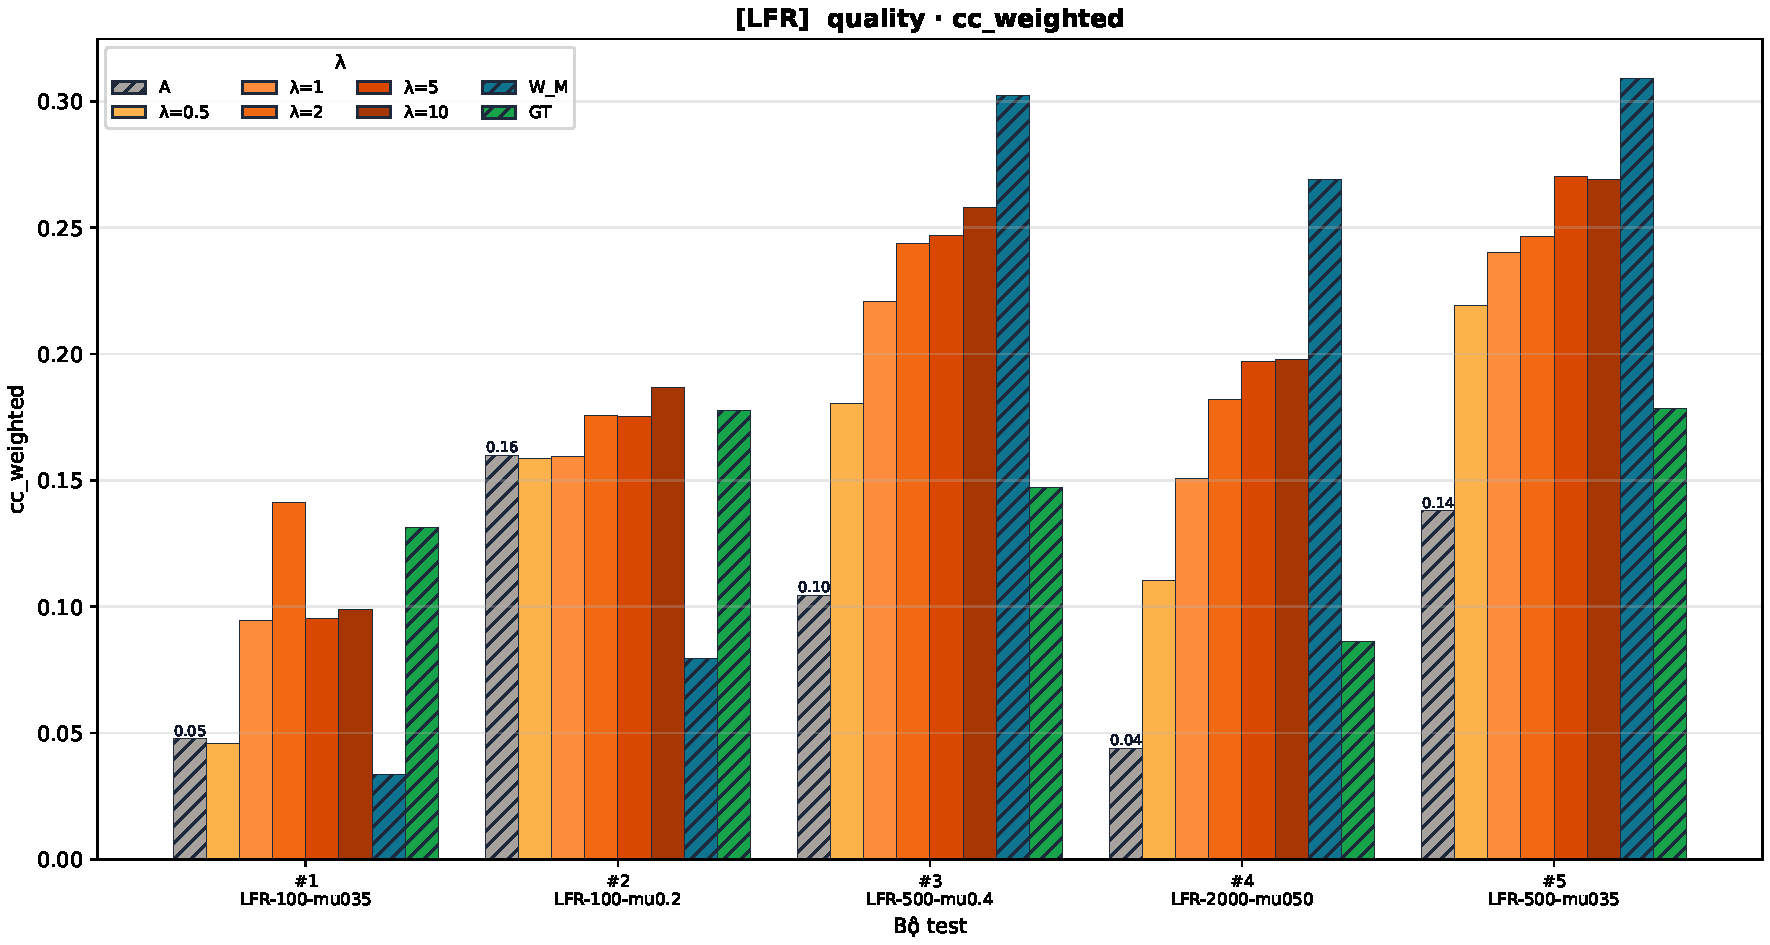
\includegraphics[width=\textwidth]{../main_result/LFR/charts/quality_cc_weighted.pdf}
    \caption{$\overline{\mathrm{CC}}_w$ trên năm bộ LFR theo $\lambda$.}
    \label{fig:lfr-cc-weighted}
\end{figure}

\begin{figure}[H]
    \centering
    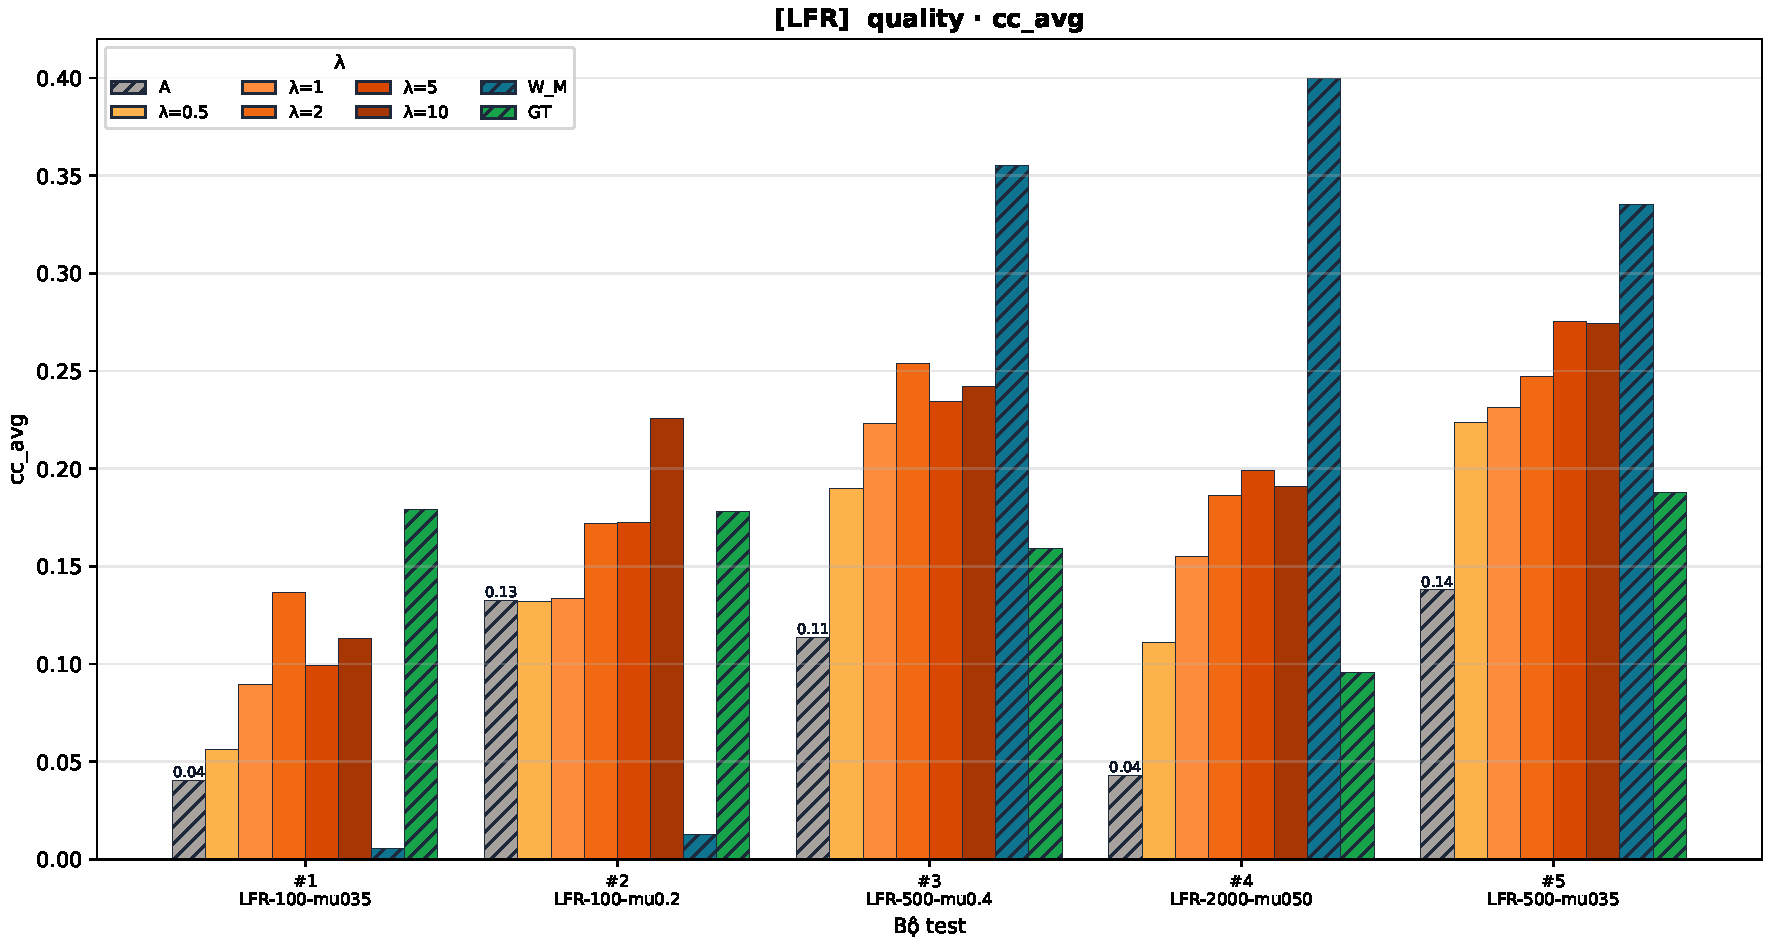
\includegraphics[width=\textwidth]{../main_result/LFR/charts/quality_cc_avg.pdf}
    \caption{$\overline{\mathrm{CC}}$ trên năm bộ LFR theo $\lambda$.}
    \label{fig:lfr-cc-avg}
\end{figure}

\textbf{Quan sát.} Hệ số phân cụm toàn cục của đồ thị gốc $cc_{\mathrm{global}} = 0{,}0513$ đóng vai trò baseline. Trên bộ LFR-100-$\mu0{,}35$, $\overline{\mathrm{CC}}_w$ chuyển từ $0{,}0477$ tại $\lambda = 0$ (sát baseline) lên cực đại $0{,}1412$ tại $\lambda = 2$, gấp khoảng ba lần. $\overline{\mathrm{CC}}$ biến thiên gần đồng pha với $\overline{\mathrm{CC}}_w$, đạt $0{,}1364$ tại $\lambda = 2$. Modularity đạt đỉnh trễ hơn, ở $\lambda = 5$.

\textbf{Nhận xét.} Việc $\overline{\mathrm{CC}}_w$ tại đỉnh vượt baseline $cc_{\mathrm{global}}$ rõ rệt cho thấy thuật toán thực sự cô lập được các vùng đậm đặc tam giác vào trong cụm, không chỉ phản ánh phân bố tam giác sẵn có của đồ thị. Lệch pha giữa đỉnh $\overline{\mathrm{CC}}_w$ và đỉnh modularity phản ánh hai khía cạnh khác nhau: $\overline{\mathrm{CC}}_w$ chỉ đo mật độ tam giác nội cụm nên tăng theo trọng số motif một cách trực tiếp, còn modularity cân bằng giữa mật độ cạnh nội cụm và kỳ vọng ngẫu nhiên, do đó phản ứng chậm hơn và chỉ đạt đỉnh khi đóng góp của motif bù trừ được tác động làm loãng cạnh gốc. Khoảng cách giữa $\overline{\mathrm{CC}}$ và $\overline{\mathrm{CC}}_w$ không đáng kể, dấu hiệu cho thấy phân bố kích thước cụm luỹ thừa của LFR không sinh ra nhiều cụm rất nhỏ đủ để làm thiên lệch trung bình không trọng số; do đó hai đại lượng cho cùng kết luận trên dataset này.

% ............................................................
\subsection{Stochastic Block Model}
\label{subsec:results-sbm}

Stochastic Block Model là mô hình tổng quát nhất trong lớp đồ thị có cấu trúc cộng đồng đối xứng. Mỗi đỉnh được gán vào một trong $K$ khối, và xác suất xuất hiện cạnh giữa hai đỉnh chỉ phụ thuộc vào cặp khối mà chúng thuộc về. Tham số then chốt là cặp $(p_{\mathrm{in}}, p_{\mathrm{out}})$ với $p_{\mathrm{in}}$ là xác suất cạnh nội cụm và $p_{\mathrm{out}}$ là xác suất cạnh liên cụm; tỉ số $p_{\mathrm{out}}/p_{\mathrm{in}}$ càng cao thì bài toán càng khó. Khoá luận quét $n \in \{300, 600, 1500, 3000\}$ với $K = 3$ và $p_{\mathrm{out}}$ thuộc $\{0{,}005,\ 0{,}008,\ 0{,}02\}$, đi kèm $p_{\mathrm{in}}$ điều chỉnh theo $n$ để giữ bậc trung bình hợp lý.

\subsubsection*{Modularity và NMI}

\begin{table}[H]
\centering
\caption{Năm bộ test SBM có cải thiện modularity lớn nhất}
\label{tab:sbm-top5}
\begin{tabular}{|l|c|c|c|c|c|c|}
\hline
\textbf{Bộ test} & $Q(0)$ & $\lambda{=}0{,}5$ & $\lambda{=}1$ & $\lambda{=}2$ & $\lambda{=}5$ & $\lambda^*$ \\ \hline
SBM-1500-$p_{\mathrm{out}}0{,}008$  & 0{,}1673 & \textbf{0{,}1975} & 0{,}1925 & 0{,}1638 & 0{,}1330 & $0{,}5$ \\ \hline
SBM-3000-$p_{\mathrm{out}}0{,}005$  & 0{,}1757 & \textbf{0{,}1951} & 0{,}1932 & 0{,}1768 & 0{,}1448 & $0{,}5$ \\ \hline
SBM-300-$p_{\mathrm{out}}0{,}02$    & 0{,}3033 & \textbf{0{,}3064} & 0{,}3016 & 0{,}2929 & 0{,}2618 & $0{,}5$ \\ \hline
SBM-600-$p_{\mathrm{out}}0{,}02$    & 0{,}2168 & \textbf{0{,}2177} & 0{,}2109 & 0{,}1907 & 0{,}1672 & $0{,}5$ \\ \hline
SBM-300-$p_{\mathrm{out}}0{,}005$   & 0{,}5497 & \textbf{0{,}5505} & 0{,}5505 & 0{,}5505 & 0{,}5505 & $0{,}5$ \\ \hline
\end{tabular}
\end{table}

\begin{figure}[H]
    \centering
    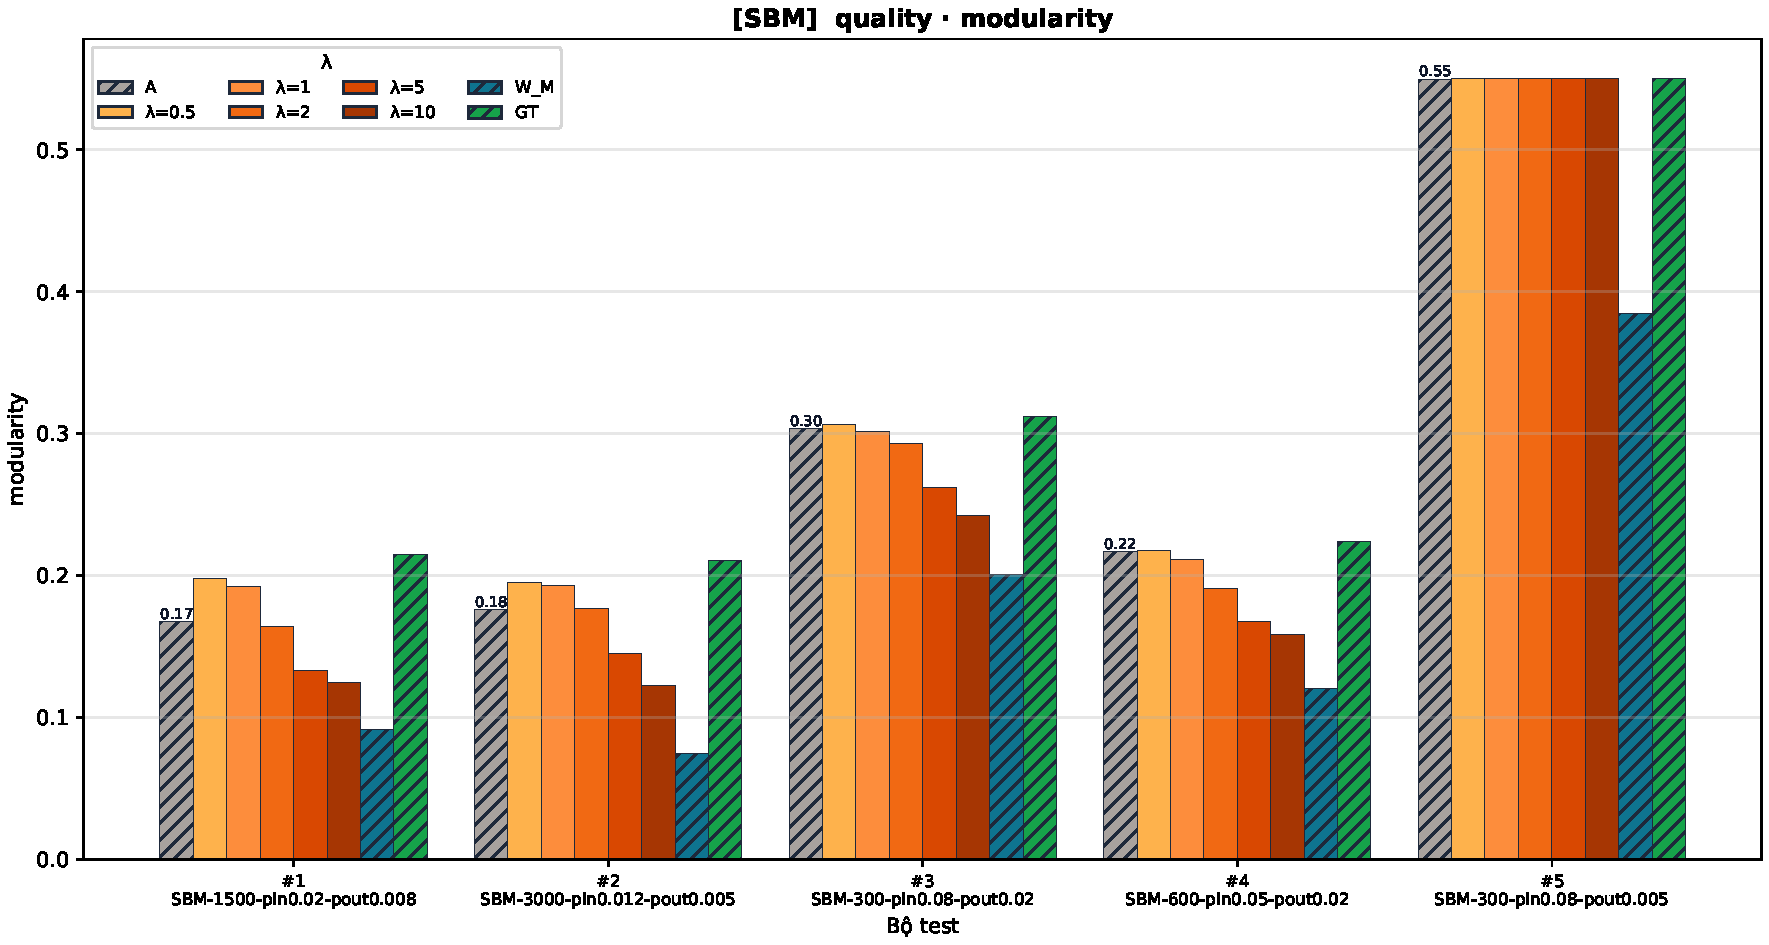
\includegraphics[width=\textwidth]{../main_result/SBM/charts/quality_modularity.pdf}
    \caption[Modularity $Q$ trên năm bộ SBM theo $\lambda$.]{Modularity $Q$ trên năm bộ SBM có $\Delta Q$ lớn nhất theo $\lambda$.}
    \label{fig:sbm-modularity}
\end{figure}

\begin{figure}[H]
    \centering
    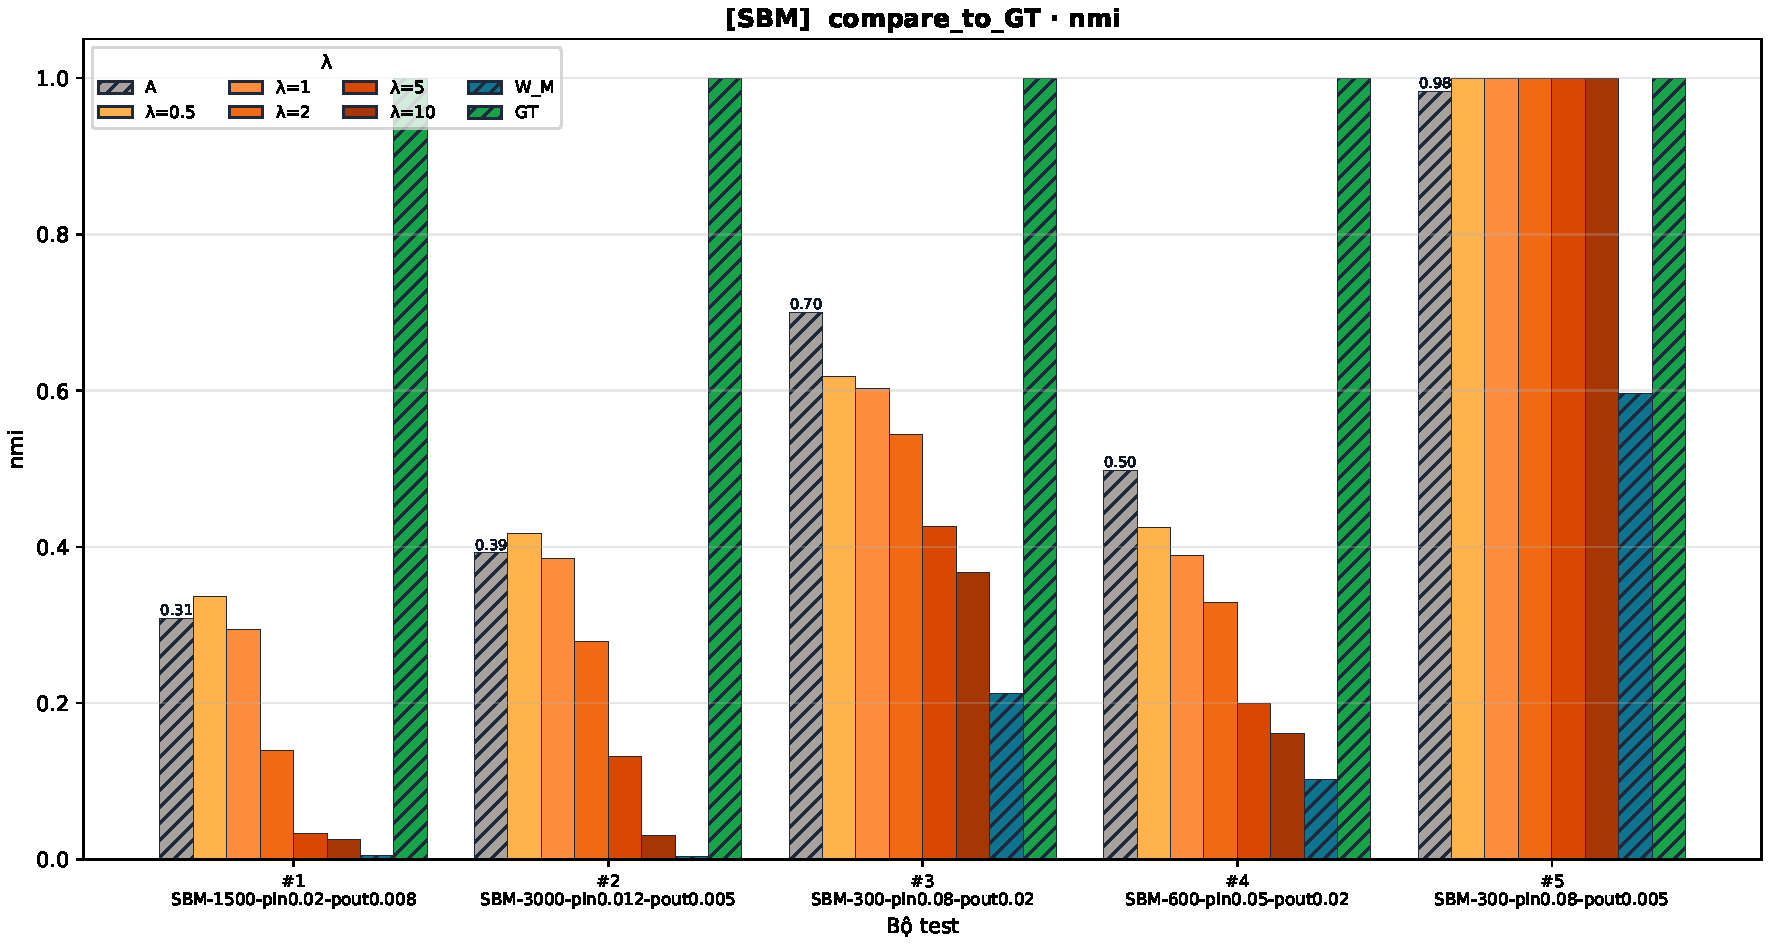
\includegraphics[width=\textwidth]{../main_result/SBM/charts/compare_to_GT_nmi.pdf}
    \caption{NMI so với phân hoạch chuẩn trên năm bộ SBM theo $\lambda$.}
    \label{fig:sbm-nmi}
\end{figure}

\textbf{Quan sát.} Toàn bộ năm bộ test cho $\lambda^* = 0{,}5$ và biên độ cải thiện $\Delta Q$ duy trì trong vùng hẹp từ $+0{,}0007$ đến $+0{,}0302$. Khi $\lambda$ vượt $0{,}5$, modularity giảm đều và NMI sụt rất nhanh: trên bộ SBM-1500-$p_{\mathrm{out}}0{,}008$, NMI từ $0{,}3360$ tại $\lambda = 0{,}5$ tụt xuống còn $0{,}0044$ tại $W_M$.

\textbf{Nhận xét.} Hành vi trên SBM khác hẳn LFR và phản ánh trực tiếp đặc tính sinh dữ liệu. Cơ chế sinh cạnh độc lập theo cặp của SBM khiến mọi tam giác xuất hiện đều là hệ quả thống kê của mật độ cạnh chứ không phải tín hiệu cấu trúc riêng. Vì thế tăng trọng số motif không cung cấp thông tin mới và còn phản tác dụng khi $\lambda$ lớn, do thành phần motif làm pha loãng tín hiệu cạnh vốn đã đủ để khôi phục cộng đồng. Sự sụp đổ nhanh của NMI là chỉ dấu rõ nhất rằng motif và phân hoạch chuẩn của SBM không chia sẻ chung một nguồn tín hiệu; bất cứ tối ưu nào theo $W_M$ thuần đều dẫn xa khỏi cộng đồng thật.

\subsubsection*{Hệ số phân cụm}

\begin{figure}[H]
    \centering
    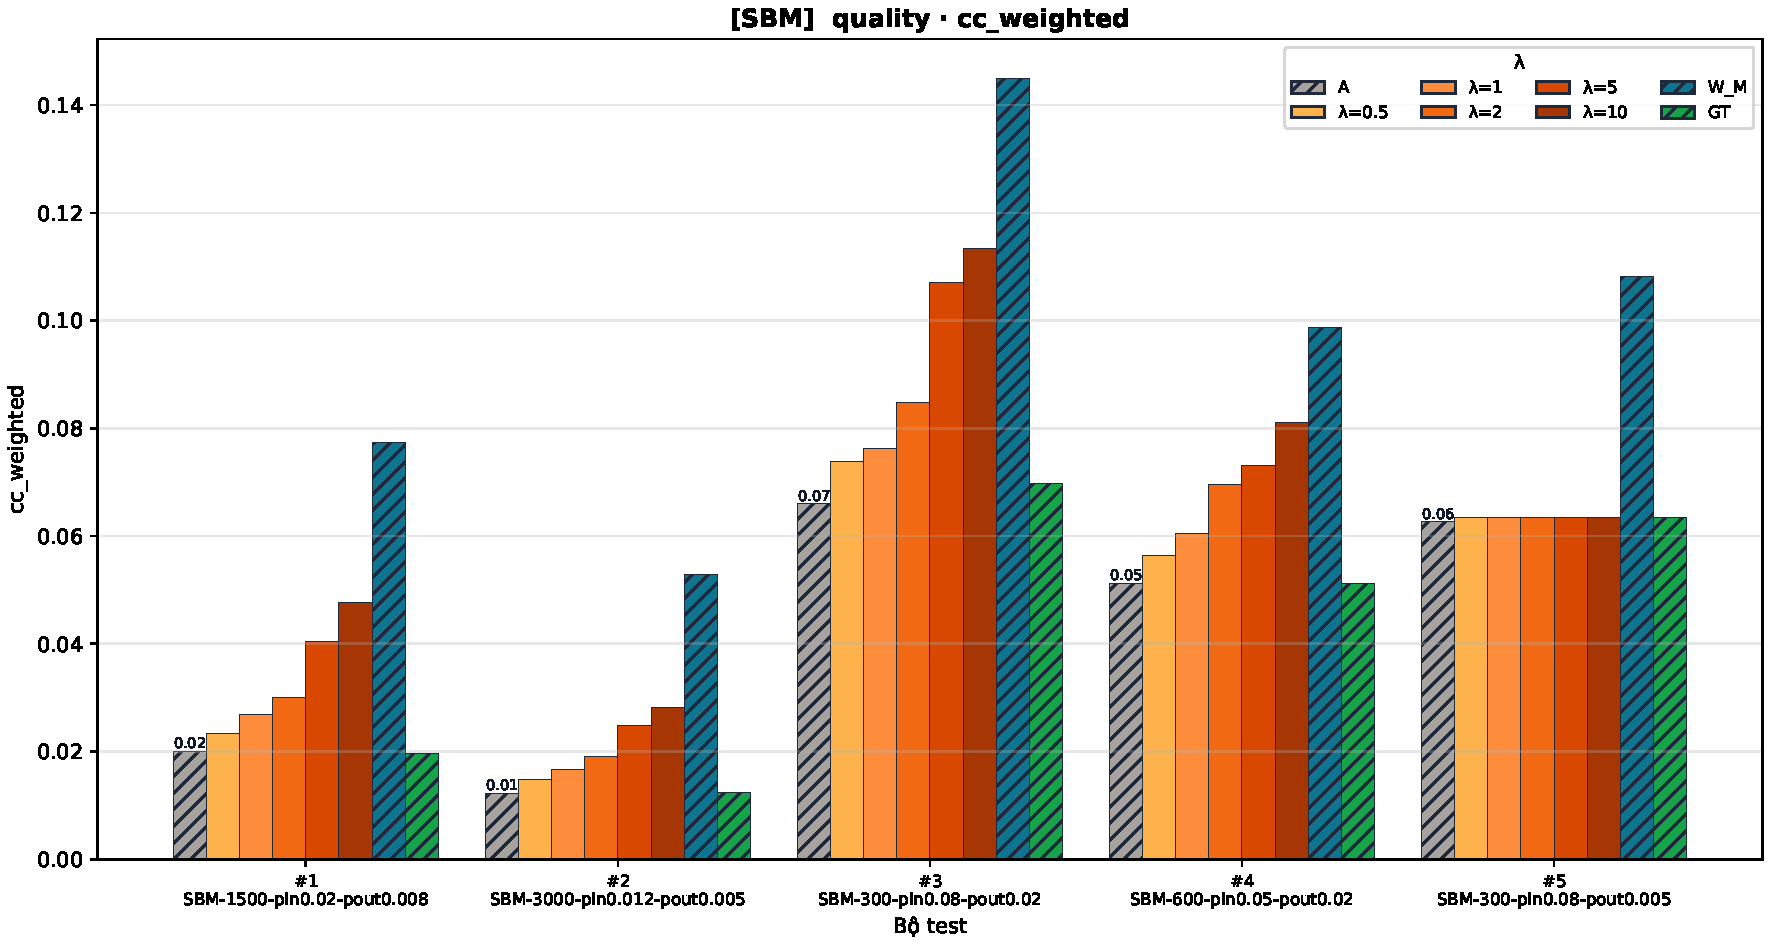
\includegraphics[width=\textwidth]{../main_result/SBM/charts/quality_cc_weighted.pdf}
    \caption{$\overline{\mathrm{CC}}_w$ trên năm bộ SBM theo $\lambda$.}
    \label{fig:sbm-cc-weighted}
\end{figure}

\begin{figure}[H]
    \centering
    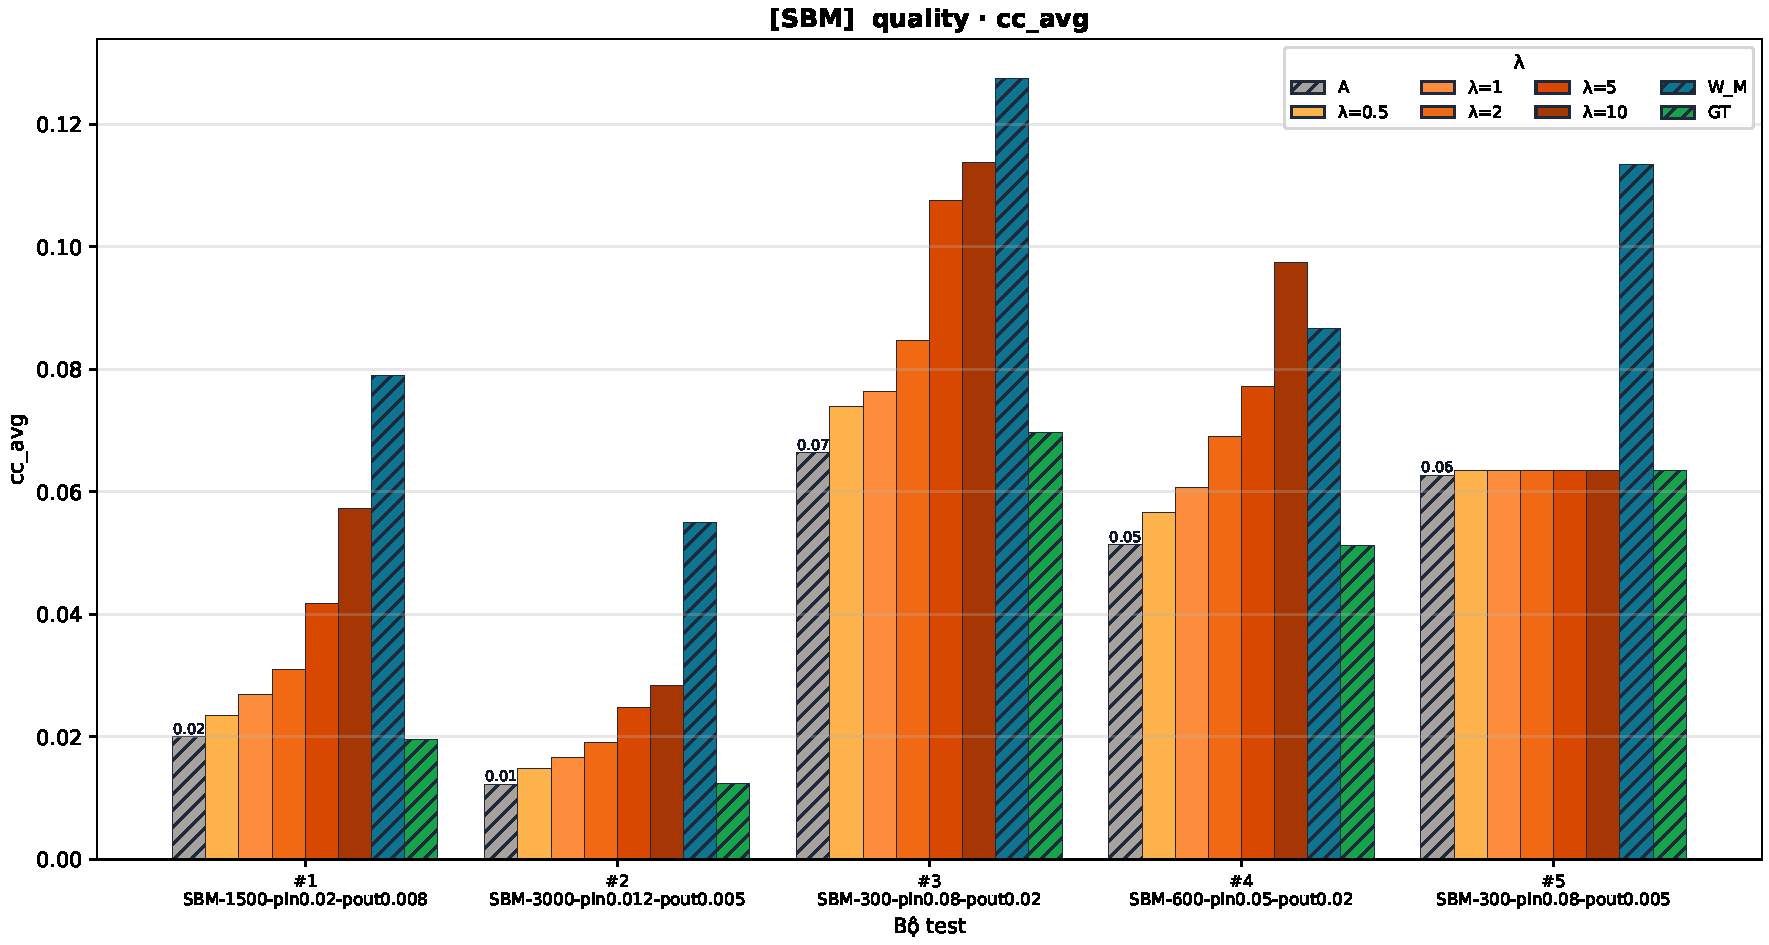
\includegraphics[width=\textwidth]{../main_result/SBM/charts/quality_cc_avg.pdf}
    \caption{$\overline{\mathrm{CC}}$ trên năm bộ SBM theo $\lambda$.}
    \label{fig:sbm-cc-avg}
\end{figure}

\textbf{Quan sát.} $cc_{\mathrm{global}} = 0{,}0128$ cho đồ thị nền của bộ SBM-1500-$p_{\mathrm{out}}0{,}008$ rất thấp, phù hợp với tính chất sinh cạnh độc lập theo cặp. Trên bộ này, $\overline{\mathrm{CC}}_w$ chuyển từ $0{,}0200$ tại $\lambda = 0$ lên $0{,}0773$ tại $W_M$, gấp khoảng sáu lần baseline. $\overline{\mathrm{CC}}$ cùng tăng đến $0{,}0791$ tại $W_M$. Cả hai đại lượng tăng đơn điệu theo $\lambda$ trên cả năm bộ test, ngược chiều biến thiên của $Q$ và NMI.

\textbf{Nhận xét.} Mức tăng tuyệt đối nhỏ ($\overline{\mathrm{CC}}_w$ tại đỉnh chỉ $0{,}0773$, thấp xa so với mức quan sát được trên LFR) phù hợp với việc SBM không sinh nhiều tam giác có nghĩa. Tỉ số $\overline{\mathrm{CC}}_w / cc_{\mathrm{global}}$ tăng chủ yếu vì baseline thấp, không phải vì thuật toán phát hiện cấu trúc tam giác đậm đặc. Sự đối lập về chiều giữa nhóm $\{\overline{\mathrm{CC}}, \overline{\mathrm{CC}}_w\}$ và nhóm $\{Q, \mathrm{NMI}\}$ mang ý nghĩa diễn giải quan trọng: dưới trọng số motif lớn, thuật toán gom được các tam giác về cùng cụm nhưng các cụm thu được lại không phản ánh phân hoạch chuẩn. Hệ quả phương pháp luận: $\overline{\mathrm{CC}}_w$, dù phản ánh đúng định nghĩa, không thể thay thế modularity hay NMI khi kiểm chứng tính đúng của phân hoạch trên SBM. Tương tự, $\overline{\mathrm{CC}}$ và $\overline{\mathrm{CC}}_w$ trùng nhau gần như chính xác, cho thấy SBM với $K = 3$ và kích thước cụm bằng nhau không có cụm nhỏ thiên lệch trung bình không trọng số.

% ............................................................
\subsection{Planted Partition}
\label{subsec:results-planted}

Planted Partition là trường hợp đặc biệt của SBM trong đó mọi cụm có cùng kích thước $s$ và mọi cặp khối dùng chung một cặp $(p_{\mathrm{in}}, p_{\mathrm{out}})$. Mức độ đối xứng cao khiến mô hình này thường được dùng làm baseline kiểm tra hành vi cơ bản của thuật toán. Khoá luận cố định $K = 5$ và quét $s \in \{40, 100, 200, 400\}$ với các cặp $(p_{\mathrm{in}}, p_{\mathrm{out}})$ tương ứng để bao quát các mức độ tách cộng đồng từ yếu đến rõ.

\subsubsection*{Modularity và NMI}

\begin{table}[H]
\centering
\caption{Bốn bộ test Planted có cải thiện modularity lớn nhất}
\label{tab:planted-top5}
\begin{tabular}{|l|c|c|c|c|c|c|}
\hline
\textbf{Bộ test} & $Q(0)$ & $\lambda{=}0{,}5$ & $\lambda{=}1$ & $\lambda{=}2$ & $\lambda{=}5$ & $\lambda^*$ \\ \hline
Planted-$s100$-$p_{\mathrm{in}}0{,}08$-$p_{\mathrm{out}}0{,}025$  & 0{,}1203 & \textbf{0{,}2185} & 0{,}2087 & 0{,}1937 & 0{,}1825 & $0{,}5$ \\ \hline
Planted-$s40$-$p_{\mathrm{in}}0{,}15$-$p_{\mathrm{out}}0{,}03$   & 0{,}2424 & \textbf{0{,}3164} & 0{,}3068 & 0{,}2862 & 0{,}2955 & $0{,}5$ \\ \hline
Planted-$s400$-$p_{\mathrm{in}}0{,}025$-$p_{\mathrm{out}}0{,}006$ & 0{,}2960 & \textbf{0{,}2974} & 0{,}2930 & 0{,}2774 & 0{,}2379 & $0{,}5$ \\ \hline
Planted-$s200$-$p_{\mathrm{in}}0{,}05$-$p_{\mathrm{out}}0{,}005$  & 0{,}5156 & \textbf{0{,}5156} & 0{,}5146 & 0{,}5107 & 0{,}5009 & $0{,}5$ \\ \hline
\end{tabular}
\end{table}

\begin{figure}[H]
    \centering
    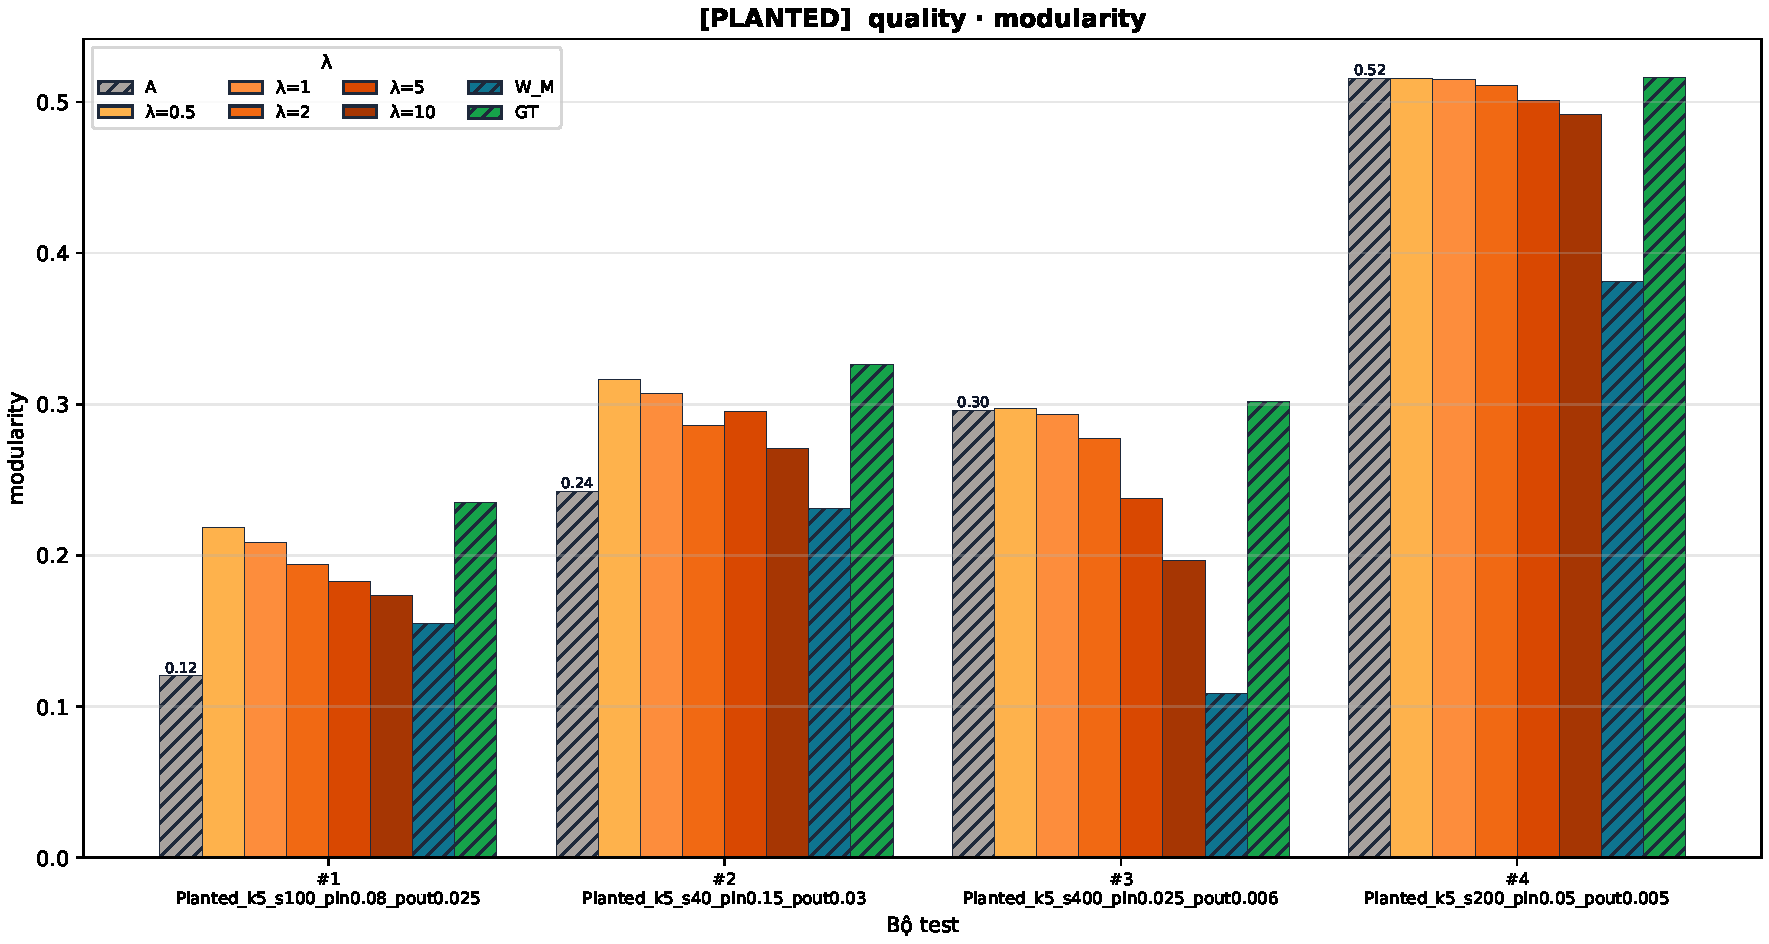
\includegraphics[width=\textwidth]{../main_result/PLANTED/charts/quality_modularity.pdf}
    \caption[Modularity $Q$ trên bốn bộ Planted Partition theo $\lambda$.]{Modularity $Q$ trên bốn bộ Planted Partition theo $\lambda$.}
    \label{fig:planted-modularity}
\end{figure}

\begin{figure}[H]
    \centering
    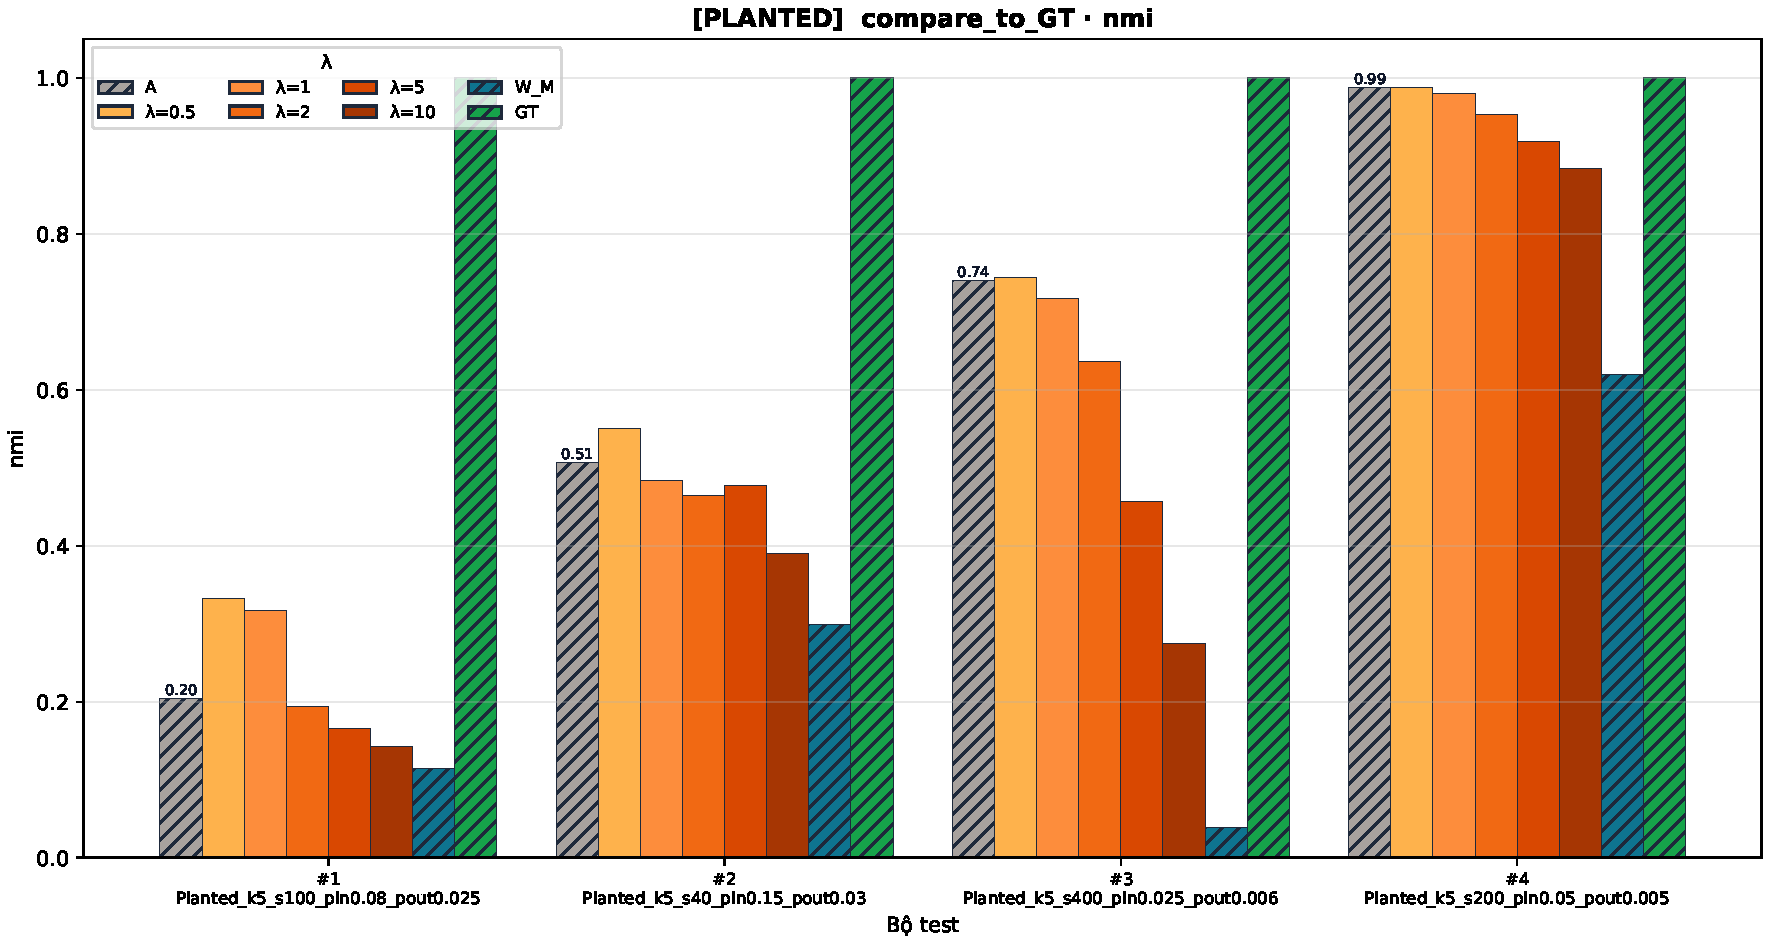
\includegraphics[width=\textwidth]{../main_result/PLANTED/charts/compare_to_GT_nmi.pdf}
    \caption{NMI so với phân hoạch chuẩn trên bốn bộ Planted Partition theo $\lambda$.}
    \label{fig:planted-nmi}
\end{figure}

\textbf{Quan sát.} $\lambda^* = 0{,}5$ trên cả bốn bộ test. Hai bộ có cộng đồng tách yếu cho $\Delta Q$ đáng kể ($+0{,}098$ và $+0{,}074$); hai bộ tách rõ gần như không cải thiện. NMI đạt đỉnh đồng thuận với modularity tại $\lambda = 0{,}5$ và giảm dần theo cùng nhịp khi $\lambda$ tăng.

\textbf{Nhận xét.} Pattern lặp lại nguyên vẹn từ SBM — điều dự kiến do Planted là trường hợp đặc biệt của SBM. Hiệu ứng bão hoà theo $Q(0)$ tỏ ra rõ rệt: khi cộng đồng đã tách rõ trong $A$, modularity ban đầu cao và phần thông tin còn lại để motif đóng góp gần như bằng không. Việc cộng đồng đối xứng, kích thước bằng nhau và xác suất sinh cạnh đồng nhất giữa các cặp khối làm cho tam giác trở thành đại lượng nhiễu thuần tuý theo nghĩa thống kê; do đó vai trò của $W^{(M)}$ chỉ dừng ở mức ổn định hoá phân cụm phổ, không bổ sung được tín hiệu cấu trúc riêng.

\subsubsection*{Hệ số phân cụm}

\begin{figure}[H]
    \centering
    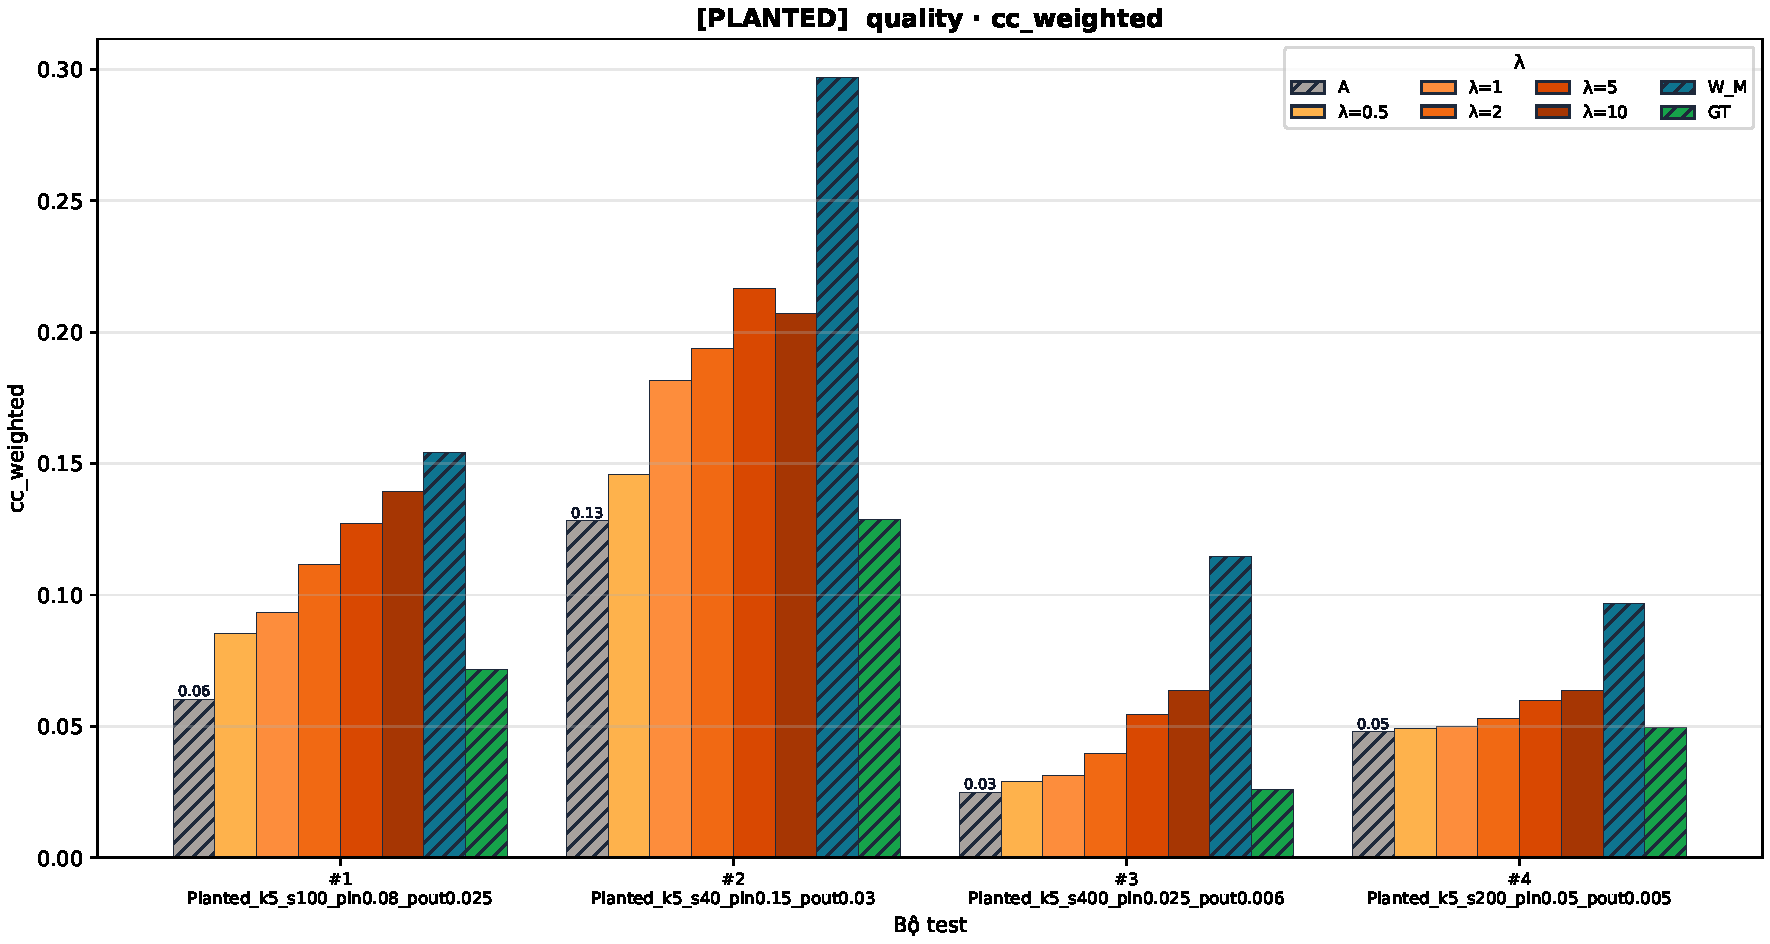
\includegraphics[width=\textwidth]{../main_result/PLANTED/charts/quality_cc_weighted.pdf}
    \caption{$\overline{\mathrm{CC}}_w$ trên bốn bộ Planted Partition theo $\lambda$.}
    \label{fig:planted-cc-weighted}
\end{figure}

\begin{figure}[H]
    \centering
    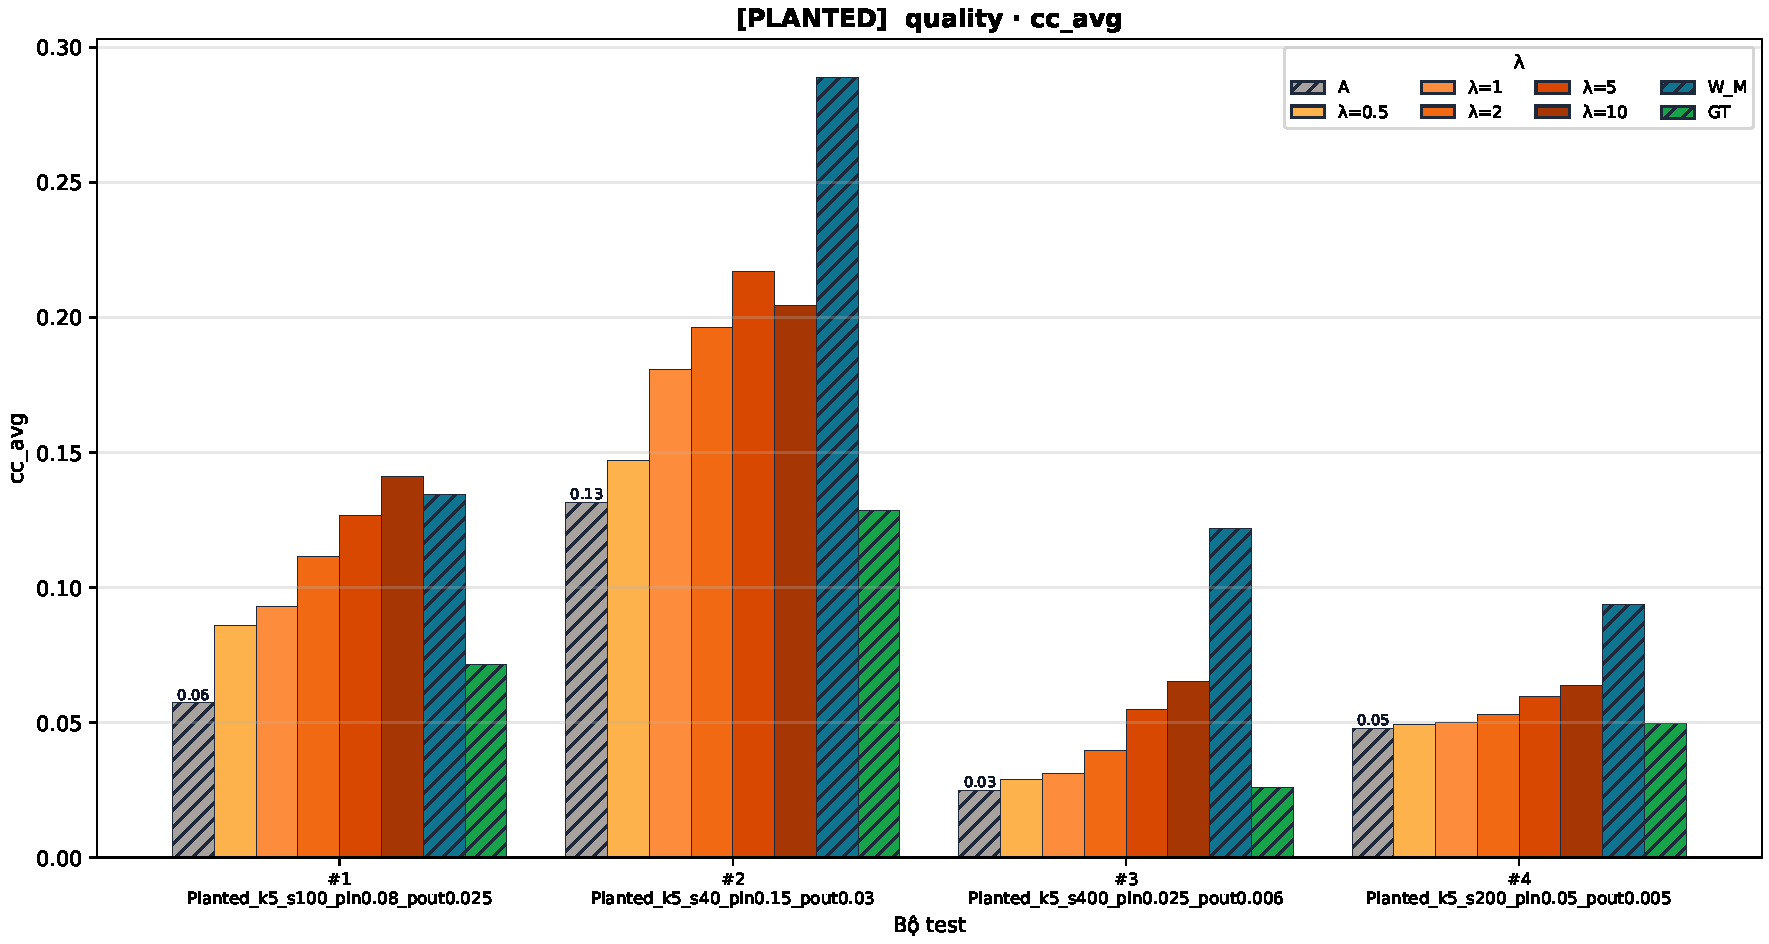
\includegraphics[width=\textwidth]{../main_result/PLANTED/charts/quality_cc_avg.pdf}
    \caption{$\overline{\mathrm{CC}}$ trên bốn bộ Planted Partition theo $\lambda$.}
    \label{fig:planted-cc-avg}
\end{figure}

\textbf{Quan sát.} $cc_{\mathrm{global}} = 0{,}0379$ cho đồ thị nền của bộ Planted-$s100$-$p_{\mathrm{in}}0{,}08$-$p_{\mathrm{out}}0{,}025$. $\overline{\mathrm{CC}}_w$ tăng từ $0{,}0604$ tại $\lambda = 0$ lên $0{,}1540$ tại $W_M$ (gấp khoảng bốn lần baseline), $\overline{\mathrm{CC}}$ đạt $0{,}1412$ tại $\lambda = 10$. Cả hai đại lượng tăng đơn điệu theo $\lambda$ trên cả bốn bộ test, trong khi $Q$ và NMI đỉnh tại $\lambda = 0{,}5$ rồi suy giảm.

\textbf{Nhận xét.} Pattern lặp lại nguyên vẹn từ SBM, điều dự kiến vì Planted là trường hợp đặc biệt của SBM. Khoảng cách hẹp giữa $\overline{\mathrm{CC}}$ và $\overline{\mathrm{CC}}_w$ là hệ quả trực tiếp của cơ chế sinh: tất cả cụm có cùng kích thước nên không có cụm nhỏ kéo trung bình không trọng số lên cao. Sự lặp lại pattern phân kỳ giữa $\{\overline{\mathrm{CC}}, \overline{\mathrm{CC}}_w\}$ và $\{Q, \mathrm{NMI}\}$ trên hai mô hình SBM và Planted khẳng định một nguyên lý chung: trên đồ thị sinh ngẫu nhiên đối xứng, mật độ tam giác nội cụm và tính đúng của phân hoạch là hai mục tiêu có thể tách biệt; tối ưu một trong hai không tự động kéo theo cải thiện đại lượng còn lại.

% ............................................................
\subsection{Gaussian Random Partition Graph}
\label{subsec:results-grpg}

Gaussian Random Partition Graph nằm giữa Planted Partition và LFR về mức độ đa dạng kích thước cụm. Kích thước mỗi cụm được lấy mẫu từ phân bố Gaussian $\mathcal{N}(s, s/v)$ với $s$ là kích thước trung bình và $v$ là tham số hình dạng kiểm soát phương sai; cạnh sau đó được sinh theo cơ chế Planted Partition trên tập cụm thu được. Khoá luận quét $n \in \{200, 500, 2000\}$ với các cặp $(p_{\mathrm{in}}, p_{\mathrm{out}})$ và $s$ tương ứng để bao quát các mức độ tách cộng đồng từ yếu đến rõ.

\subsubsection*{Modularity và NMI}

\begin{table}[H]
\centering
\caption{Năm bộ test GRPG có cải thiện modularity lớn nhất}
\label{tab:grpg-top5}
\begin{tabular}{|l|c|c|c|c|c|c|}
\hline
\textbf{Bộ test} & $Q(0)$ & $\lambda{=}0{,}5$ & $\lambda{=}1$ & $\lambda{=}2$ & $\lambda{=}5$ & $\lambda^*$ \\ \hline
GRPG-2000-$p_{\mathrm{out}}0{,}006$ & 0{,}1165 & 0{,}2004 & \textbf{0{,}2005} & 0{,}1887 & 0{,}1678 & $1{,}0$ \\ \hline
GRPG-500-$p_{\mathrm{out}}0{,}008$  & 0{,}4240 & \textbf{0{,}4753} & 0{,}4728 & 0{,}4668 & 0{,}4590 & $0{,}5$ \\ \hline
GRPG-500-$p_{\mathrm{out}}0{,}015$  & 0{,}2914 & \textbf{0{,}3400} & 0{,}3307 & 0{,}3113 & 0{,}3026 & $0{,}5$ \\ \hline
GRPG-2000-$p_{\mathrm{out}}0{,}001$ & 0{,}6209 & \textbf{0{,}6611} & 0{,}6196 & 0{,}6600 & 0{,}6573 & $0{,}5$ \\ \hline
GRPG-200-$p_{\mathrm{out}}0{,}03$   & 0{,}3593 & \textbf{0{,}3606} & 0{,}3572 & 0{,}3523 & 0{,}3436 & $0{,}5$ \\ \hline
\end{tabular}
\end{table}

\begin{figure}[H]
    \centering
    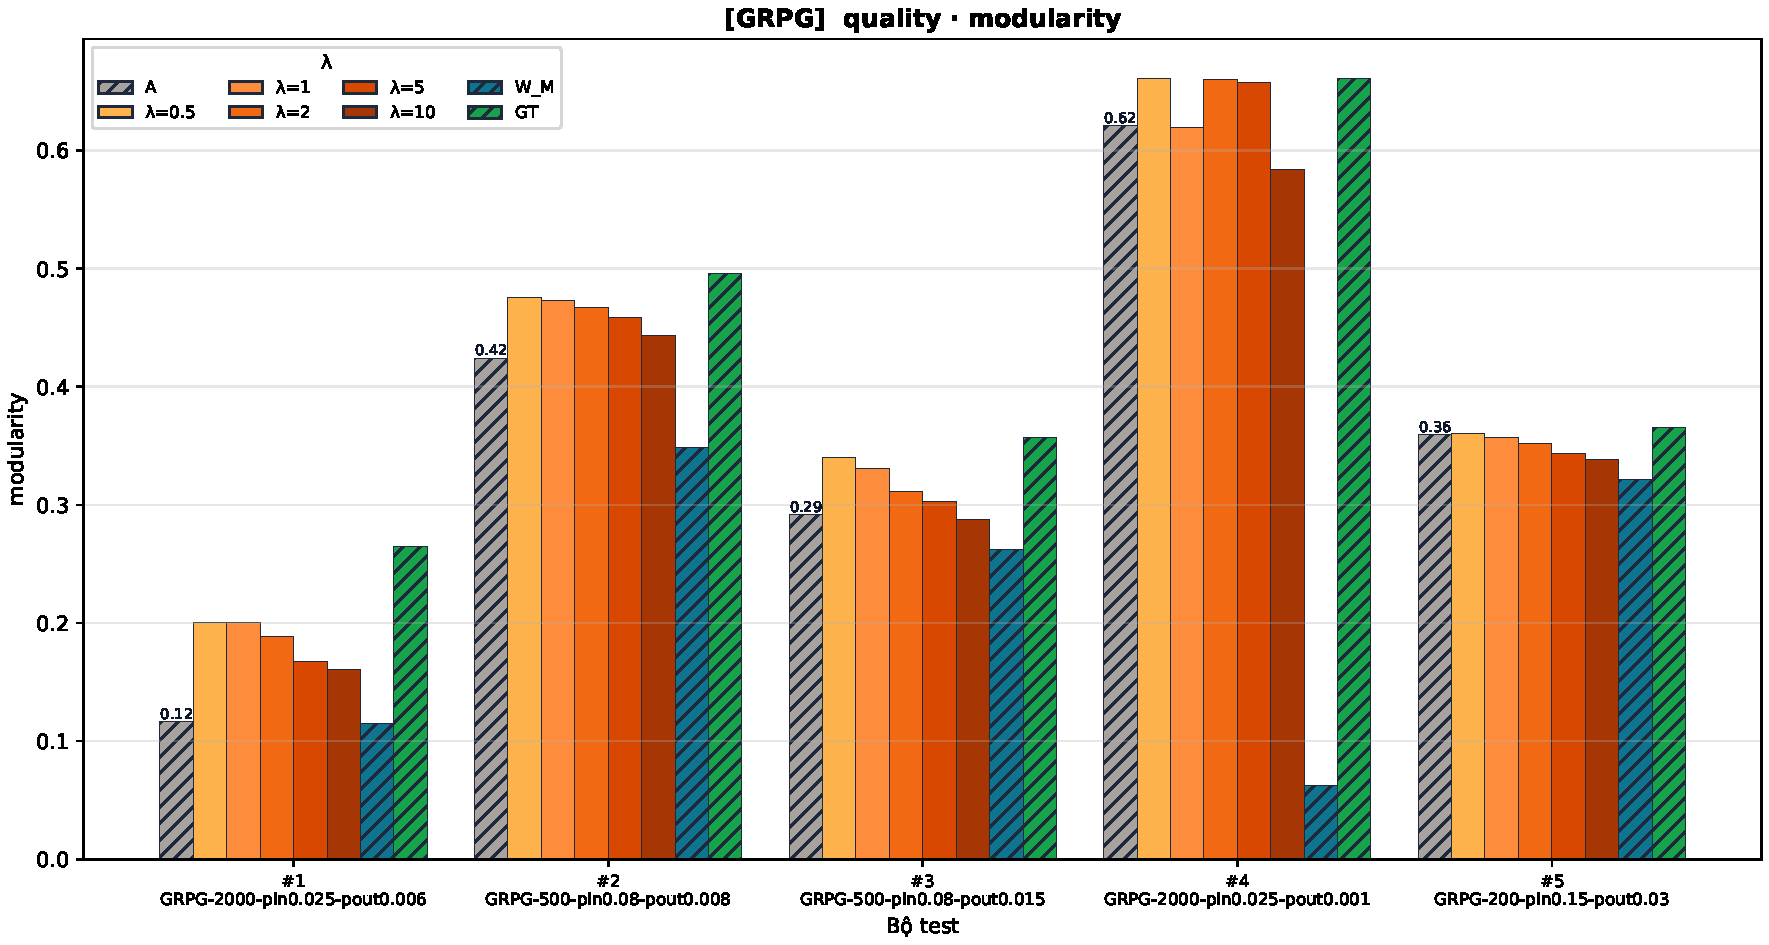
\includegraphics[width=\textwidth]{../main_result/GRPG/charts/quality_modularity.pdf}
    \caption[Modularity $Q$ trên năm bộ GRPG theo $\lambda$.]{Modularity $Q$ trên năm bộ GRPG theo $\lambda$.}
    \label{fig:grpg-modularity}
\end{figure}

\begin{figure}[H]
    \centering
    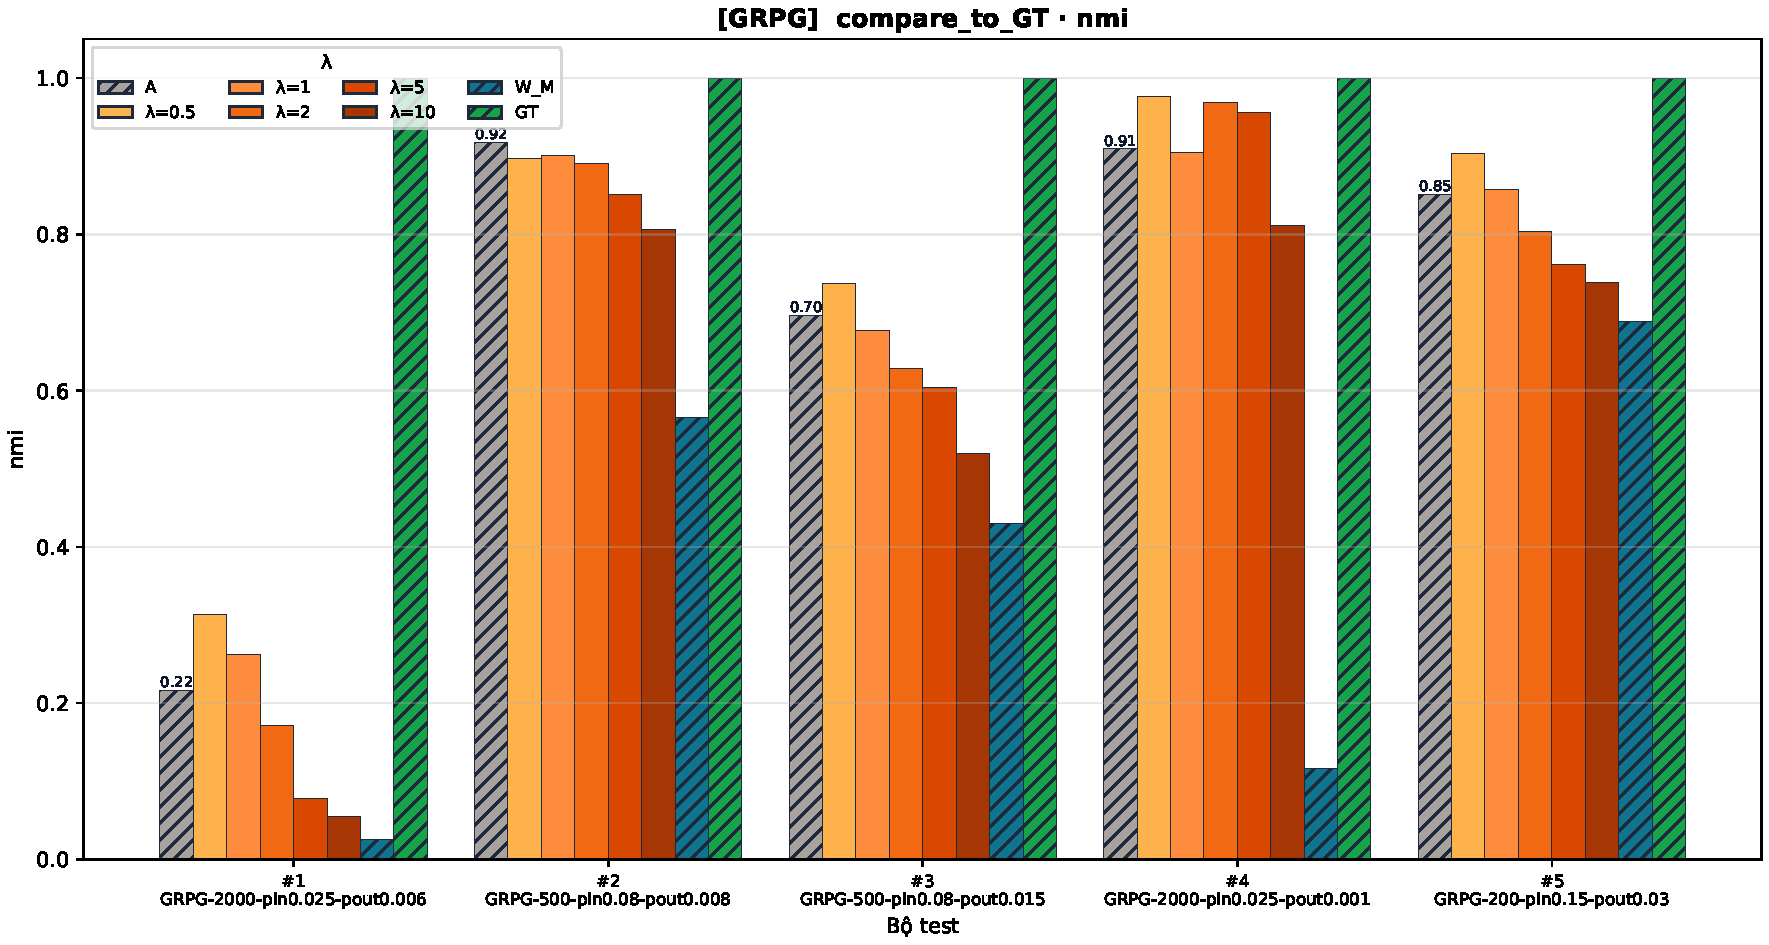
\includegraphics[width=\textwidth]{../main_result/GRPG/charts/compare_to_GT_nmi.pdf}
    \caption{NMI so với phân hoạch chuẩn trên năm bộ GRPG theo $\lambda$.}
    \label{fig:grpg-nmi}
\end{figure}

\textbf{Quan sát.} $\lambda^*$ luôn thuộc $\{0{,}5, 1\}$, nhưng biên độ cải thiện vượt Planted: bộ GRPG-2000-$p_{\mathrm{out}}0{,}006$ cho $\Delta Q = +0{,}0840$, cùng cấp độ với các bộ LFR khó nhất. NMI đạt đỉnh tại $\lambda = 0{,}5$, sớm hơn modularity (đỉnh tại $\lambda = 1$) một bước.

\textbf{Nhận xét.} GRPG cho hành vi trung gian giữa Planted và LFR. Sự đa dạng về kích thước cụm sinh ra từ phân bố Gaussian dường như mở rộng phạm vi $\lambda$ mà motif còn đóng góp tích cực, đẩy biên độ cải thiện vượt Planted dù chưa đủ để $\lambda^*$ vượt khỏi vùng nhỏ. Sự lệch pha một bước giữa đỉnh NMI và đỉnh modularity là cảnh báo phương pháp luận: ngay trong vùng cải thiện, phân hoạch tối ưu theo modularity đã bắt đầu rời khỏi phân hoạch chuẩn. Việc dựa hoàn toàn vào modularity để chọn $\lambda^*$ có thể dẫn đến phân hoạch lệch khỏi ground truth dù $\Delta Q$ vẫn dương.

\subsubsection*{Hệ số phân cụm}

\begin{figure}[H]
    \centering
    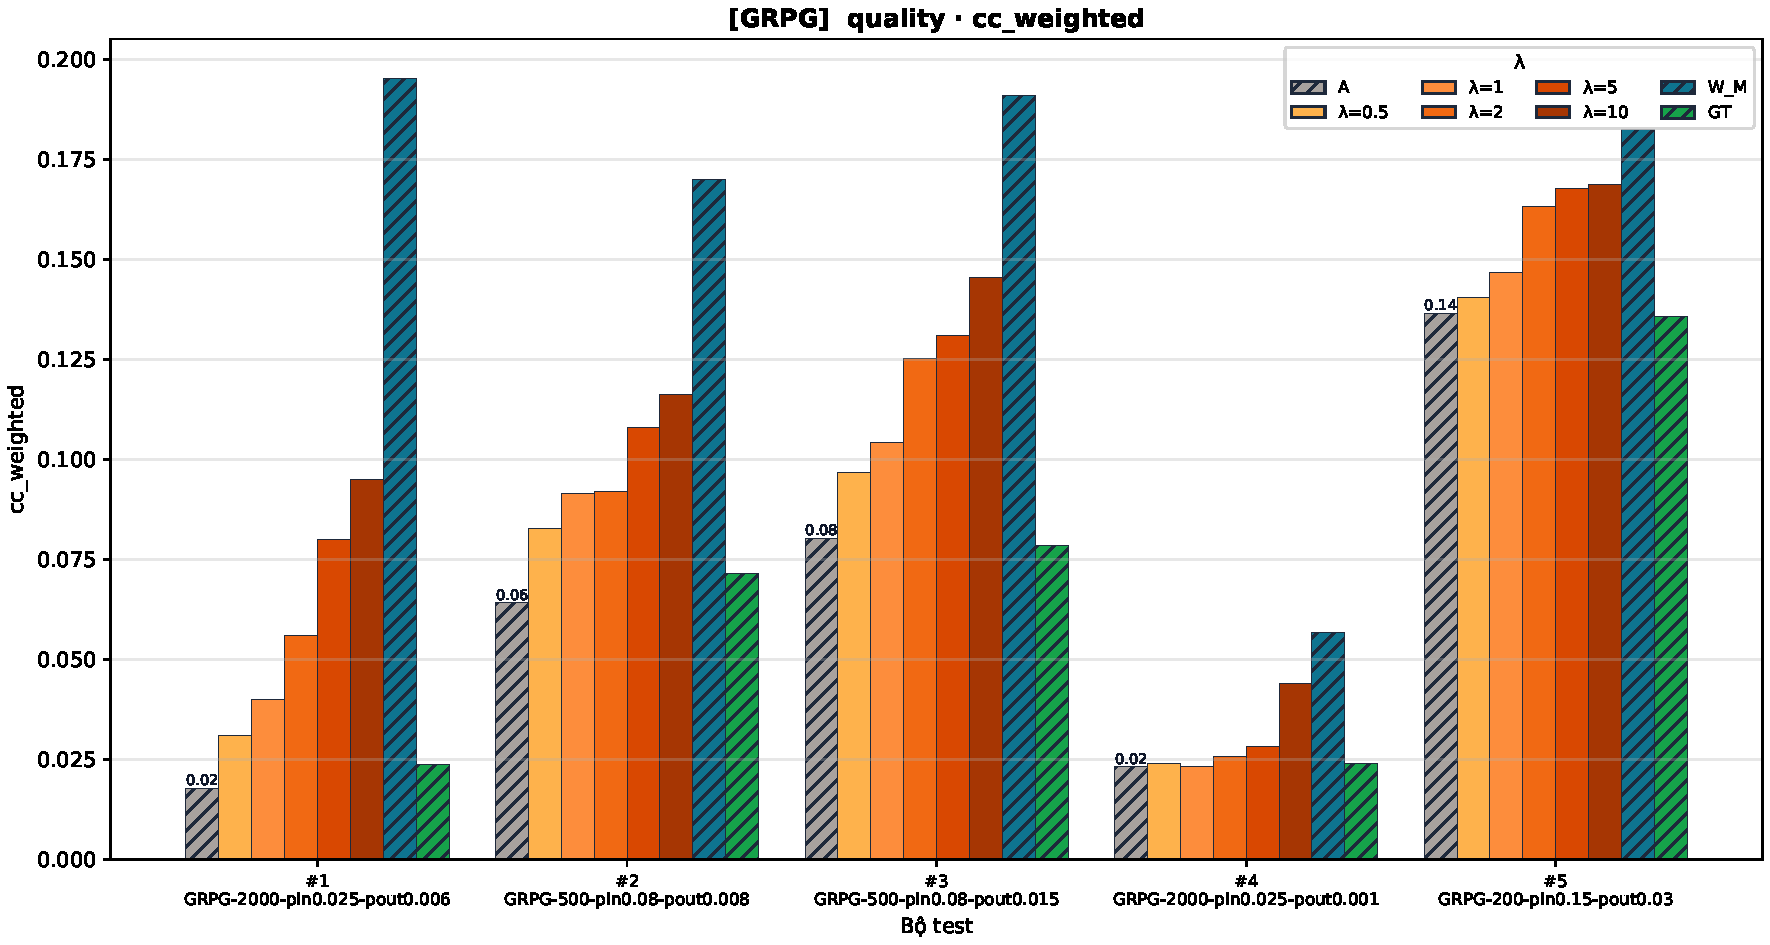
\includegraphics[width=\textwidth]{../main_result/GRPG/charts/quality_cc_weighted.pdf}
    \caption{$\overline{\mathrm{CC}}_w$ trên năm bộ GRPG theo $\lambda$.}
    \label{fig:grpg-cc-weighted}
\end{figure}

\begin{figure}[H]
    \centering
    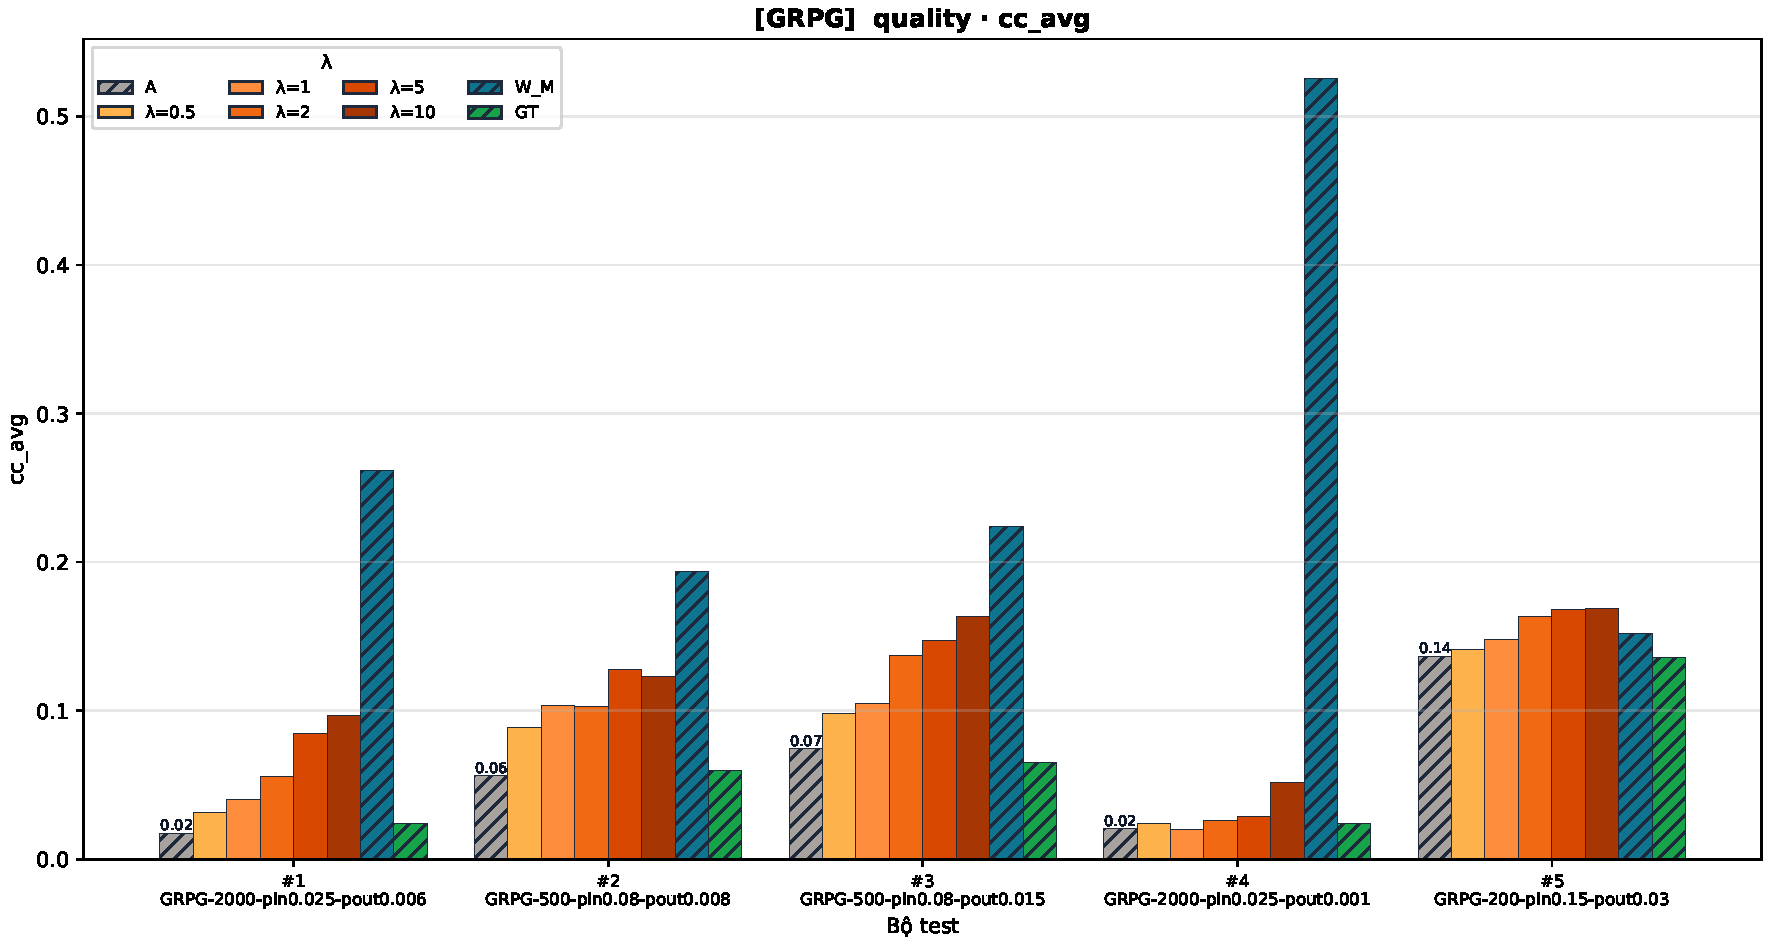
\includegraphics[width=\textwidth]{../main_result/GRPG/charts/quality_cc_avg.pdf}
    \caption{$\overline{\mathrm{CC}}$ trên năm bộ GRPG theo $\lambda$.}
    \label{fig:grpg-cc-avg}
\end{figure}

\textbf{Quan sát.} $cc_{\mathrm{global}} = 0{,}0104$ cho đồ thị nền của bộ GRPG-2000-$p_{\mathrm{out}}0{,}006$, ở mức rất thấp tương tự SBM. Trên bộ này, $\overline{\mathrm{CC}}_w$ tăng từ $0{,}0178$ tại $\lambda = 0$ lên $0{,}1953$ tại $W_M$, gấp khoảng mười một lần baseline. $\overline{\mathrm{CC}}$ đạt $0{,}2617$ tại $W_M$, cách $\overline{\mathrm{CC}}_w$ một khoảng đáng kể.

\textbf{Nhận xét.} Mức tăng tuyệt đối của $\overline{\mathrm{CC}}_w$ vượt trội so với SBM và Planted, phản ánh khả năng thuật toán cô lập các vùng tam giác đậm đặc khi phân bố kích thước cụm đa dạng. Khoảng cách rõ rệt giữa $\overline{\mathrm{CC}}$ và $\overline{\mathrm{CC}}_w$ tại $W_M$ là đặc trưng của GRPG: phân bố Gaussian sinh ra một số cụm kích thước nhỏ với hệ số phân cụm cao trên đơn vị đỉnh, làm thiên lệch trung bình không trọng số lên cao. Đây là minh hoạ thực nghiệm rõ nhất cho lý do khoá luận chọn $\overline{\mathrm{CC}}_w$ làm chỉ số chính (Định nghĩa~\ref{def:cc-cluster}): trên các đồ thị có kích thước cụm đa dạng, $\overline{\mathrm{CC}}$ có thể đánh giá quá lạc quan do hiệu ứng cụm nhỏ. Mặc dù vậy, pattern cốt lõi vẫn được giữ — cực đại của $\overline{\mathrm{CC}}_w$ không trùng cực đại của modularity, khẳng định tách biệt giữa hai mục tiêu trên lớp đồ thị sinh ngẫu nhiên đối xứng.

% ============================================================
\section{Đồ thị mạng xã hội thật}
\label{sec:results-real}

Mười một đồ thị thật được khảo sát với $\lambda \in \{0,\ 1,\ 5,\ 10,\ W_M\}$ và $K$ quét trong $\{50, 100, 200, 300, 400, 500\}$. Mỗi đồ thị có ý nghĩa đỉnh và cạnh riêng, dẫn đến đặc tính cấu trúc khác nhau. Bảng~\ref{tab:real-summary} tổng hợp bộ test có $\Delta Q$ cao nhất cho mỗi đồ thị, sau đó từng đồ thị được trình bày kèm biểu đồ chi tiết.

\begin{table}[H]
\centering
\small
\caption{Tổng hợp kết quả trên mười đồ thị mạng xã hội thật}
\label{tab:real-summary}
\begin{tabular}{|l|r|r|c|c|c|r|}
\hline
\textbf{Đồ thị} & $n$ & $m$ & $cc_{\mathrm{global}}$ & $K^*$ & $\lambda^*$ & $\Delta Q$ \\ \hline
musae\_DE\_edges    & 9{,}498   & 153{,}138 & 0{,}2009 & 50  & $W_M$ & $+0{,}1156$ \\ \hline
musae\_ES\_edges    & 4{,}648   & 59{,}382  & 0{,}2225 & 50  & $1{,}0$  & $+0{,}0902$ \\ \hline
lastfm\_asia\_edges & 7{,}624   & 27{,}806  & 0{,}2194 & 500 & $10{,}0$ & $+0{,}0815$ \\ \hline
Email-Enron         & 33{,}696  & 180{,}811 & 0{,}5092 & 300 & $5{,}0$  & $+0{,}0640$ \\ \hline
facebook\_combined  & 4{,}039   & 88{,}234  & 0{,}6055 & 500 & $5{,}0$  & $+0{,}0519$ \\ \hline
CA-GrQc             & 4{,}158   & 13{,}422  & 0{,}5569 & 500 & $5{,}0$  & $+0{,}0476$ \\ \hline
CA-AstroPh          & 17{,}903  & 196{,}972 & 0{,}6328 & 50  & $5{,}0$  & $+0{,}0421$ \\ \hline
CA-CondMat          & 21{,}363  & 91{,}286  & 0{,}6417 & 50  & $5{,}0$  & $+0{,}0316$ \\ \hline
CA-HepTh            & 8{,}638   & 24{,}806  & 0{,}4816 & 50  & $5{,}0$  & $+0{,}0250$ \\ \hline
musae\_facebook\_edges & 22{,}470 & 170{,}823 & 0{,}3597 & 500 & $5{,}0$ & $+0{,}0202$ \\ \hline
\end{tabular}
\end{table}

% ............................................................
\subsection*{musae\_DE}

Đỉnh là một streamer Twitch người Đức, cạnh nối hai streamer cùng chia sẻ người theo dõi. Cộng đồng có nghĩa là nhóm streamer cùng phân khúc khán giả. Hệ số phân cụm toàn cục $cc_{\mathrm{global}} = 0{,}2009$ ở mức trung bình.

\textbf{Modularity.}
\begin{figure}[H]
    \centering
    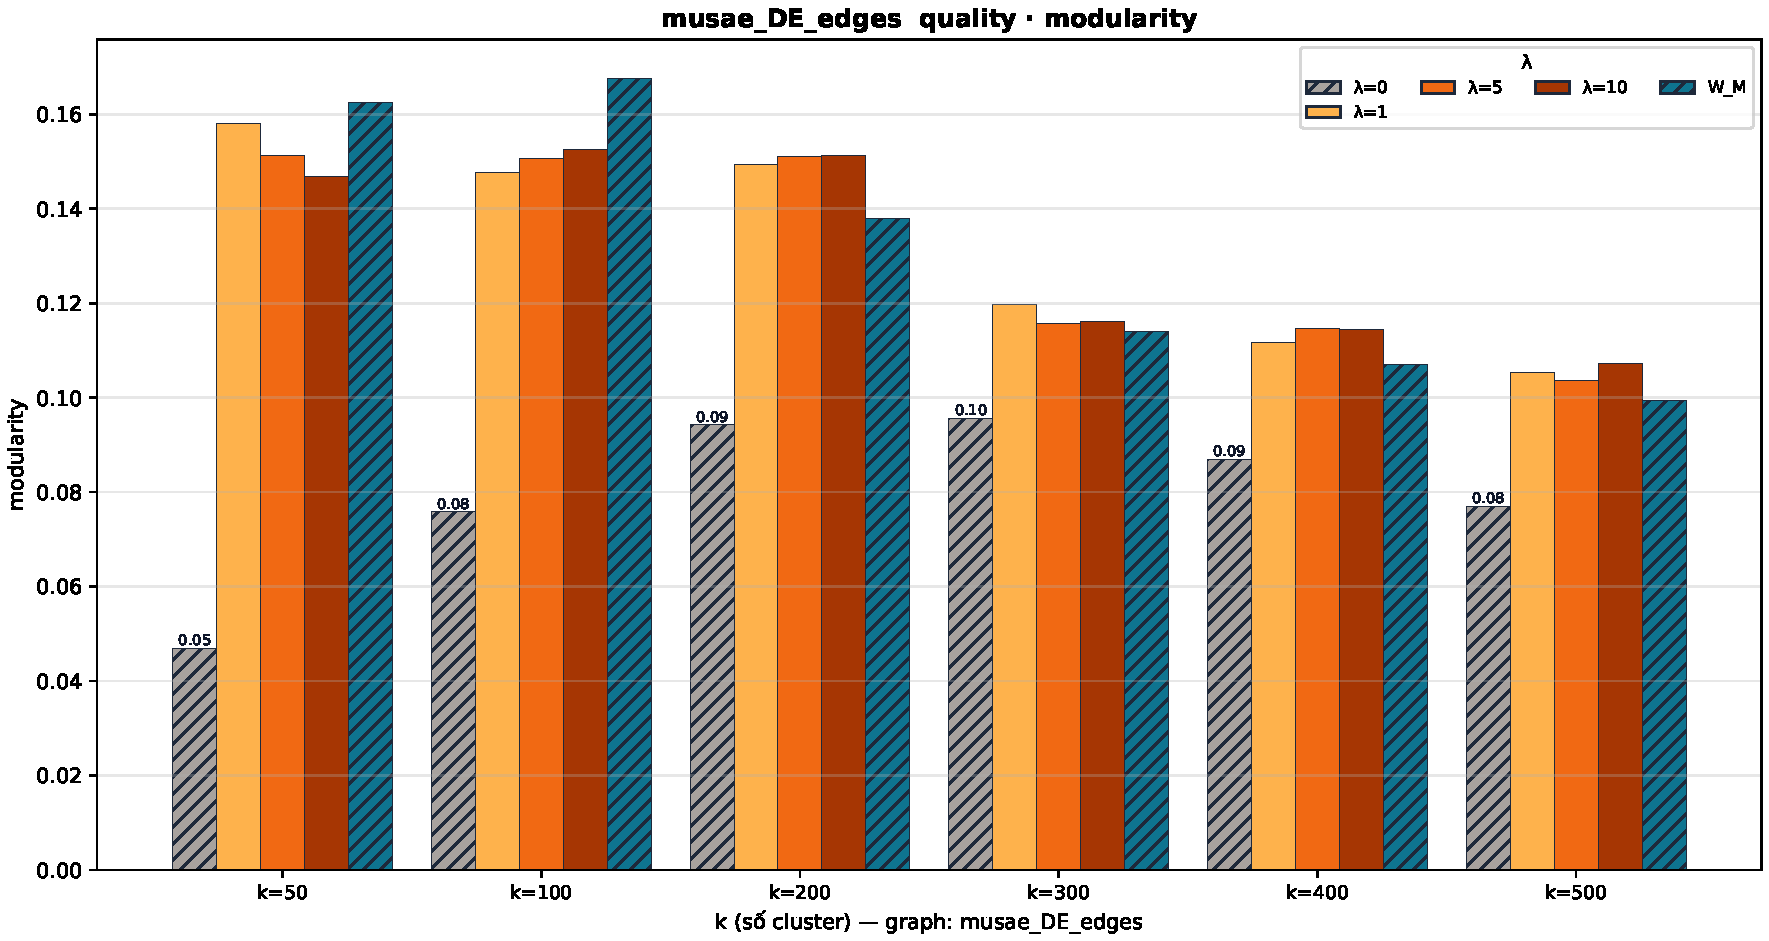
\includegraphics[width=\textwidth]{../main_result/REAL/musae_DE_edges/charts/quality_modularity.pdf}
    \caption{Modularity $Q$ trên musae\_DE theo $\lambda$ và $K$.}
    \label{fig:real-musae-de}
\end{figure}

$Q(0)$ rất thấp trên mọi $K$ (chỉ trong khoảng $0{,}05$--$0{,}10$). Ma trận hỗn hợp đẩy $Q$ lên gấp hai đến ba lần, mạnh nhất tại $K = 50$ với $\Delta Q = +0{,}1156$ và $\lambda^* = W_M$. Đây là trường hợp $Q(0)$ thấp điển hình: phân cụm phổ trên $A$ thuần không tìm được phân hoạch tốt, trọng số motif lớn tạo ra cải thiện rõ rệt.

\textbf{Hệ số phân cụm.}
\begin{figure}[H]
    \centering
    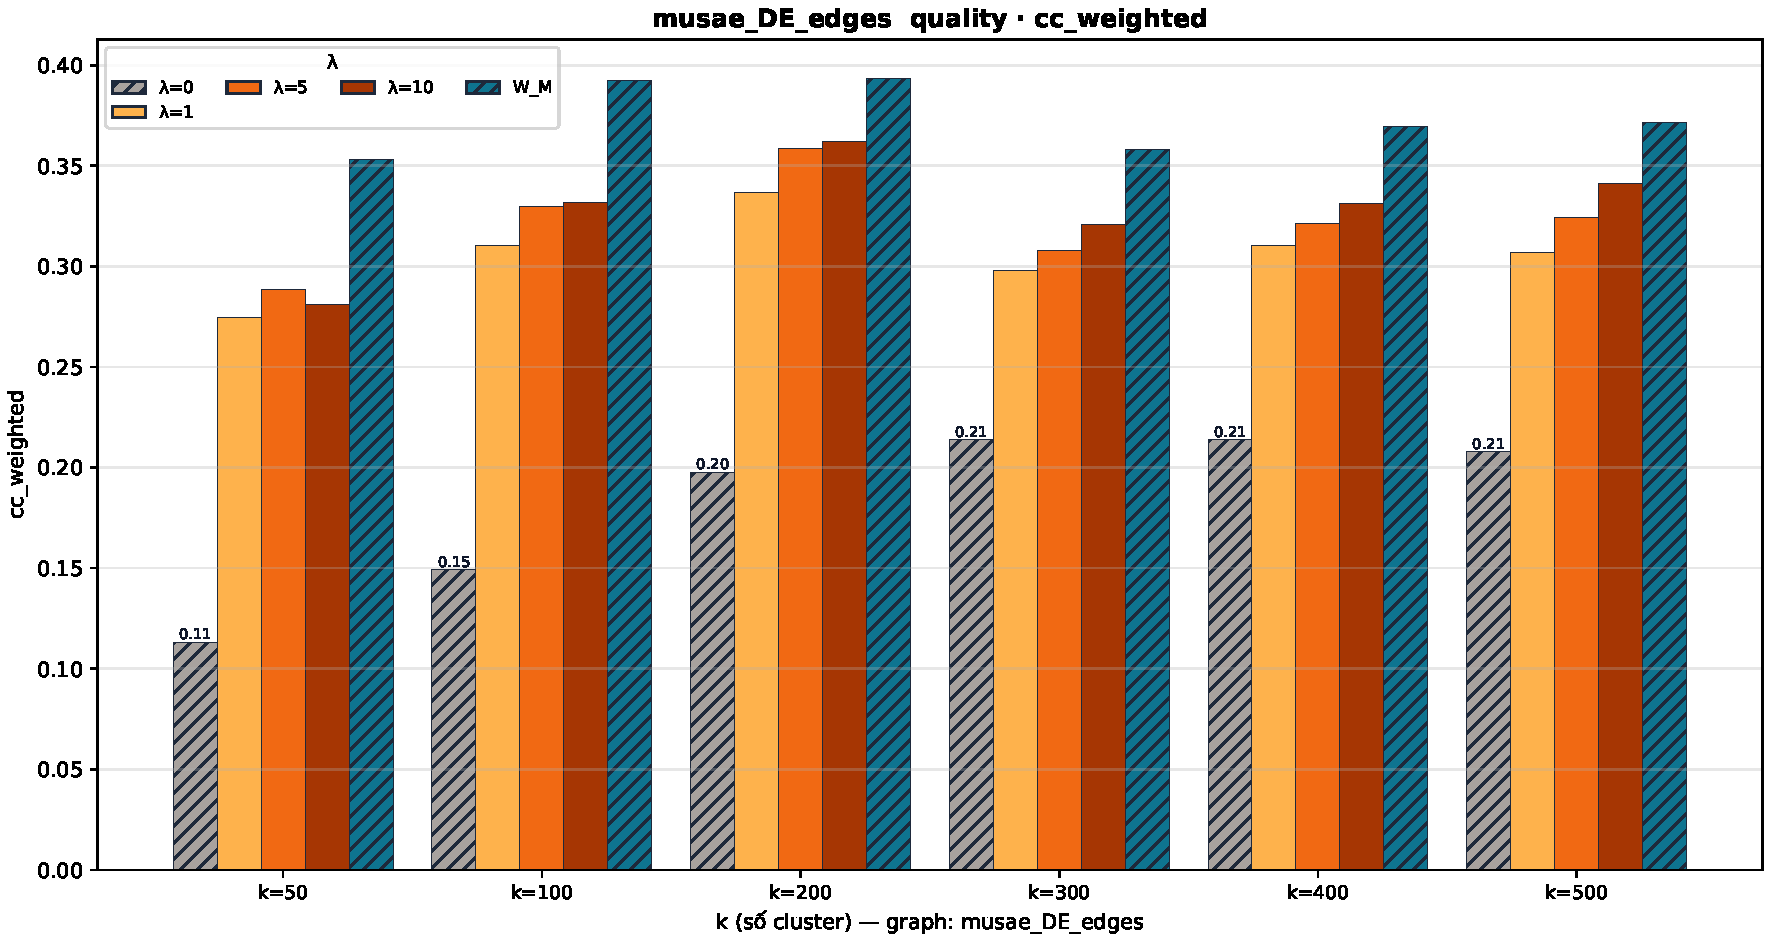
\includegraphics[width=\textwidth]{../main_result/REAL/musae_DE_edges/charts/quality_cc_weighted.pdf}
    \caption{$\overline{\mathrm{CC}}_w$ trên musae\_DE theo $\lambda$ và $K$.}
    \label{fig:real-cc-musae-de}
\end{figure}

\begin{figure}[H]
    \centering
    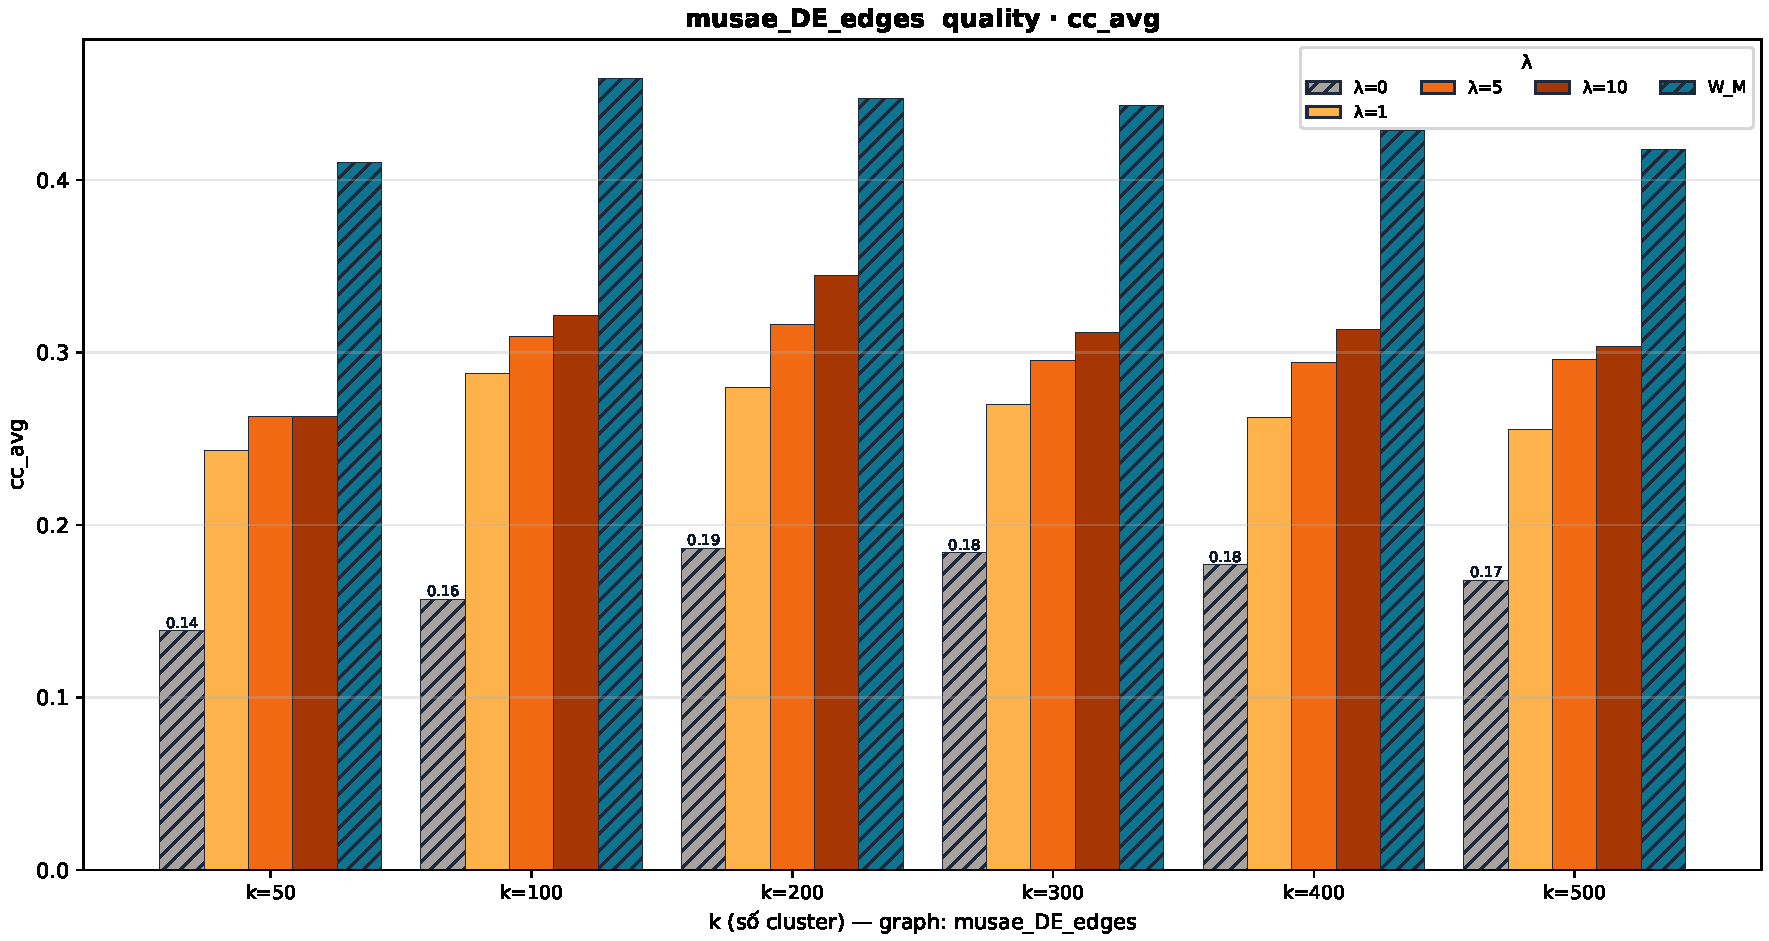
\includegraphics[width=\textwidth]{../main_result/REAL/musae_DE_edges/charts/quality_cc_avg.pdf}
    \caption{$\overline{\mathrm{CC}}$ trên musae\_DE theo $\lambda$ và $K$.}
    \label{fig:real-ccavg-musae-de}
\end{figure}

Tại $K = 50$, $\overline{\mathrm{CC}}_w(0) = 0{,}1132$ thấp hơn cả $cc_{\mathrm{global}}$, nghĩa là phân cụm phổ trên $A$ không gom được tam giác có sẵn vào trong cụm. Khi $\lambda$ chuyển về $W_M$, $\overline{\mathrm{CC}}_w$ đạt $0{,}3531$, gấp ba lần và vượt baseline $cc_{\mathrm{global}}$. $\overline{\mathrm{CC}}$ cũng tăng lên $0{,}4103$ tại $W_M$, bật từ $0{,}2630$ tại $\lambda = 10$ (tăng $0{,}15$ chỉ qua một bước sang $W_M$); $\overline{\mathrm{CC}}_w$ trong cùng đoạn chỉ tăng từ $0{,}2810$ lên $0{,}3531$, độ tăng nhỏ hơn rõ rệt. Điều này phù hợp với nhận định ở Định nghĩa~\ref{def:cc-cluster}: việc bỏ ma trận kề $A$ tạo ra một số cụm rất nhỏ với $\mathrm{CC}$ cục bộ cao, đẩy $\overline{\mathrm{CC}}$ lên trong khi $\overline{\mathrm{CC}}_w$ vẫn phản ánh trung thực kích thước cụm trung bình.

\textbf{Kết luận.} musae\_DE đại diện cho lớp đồ thị xã hội với triadic closure mạnh nhưng cộng đồng được mã hoá ẩn trong cấu trúc tam giác, không thể phát hiện chỉ qua cạnh. Trọng số motif lớn ($W_M$) là cần thiết để bóc tách cộng đồng; cả modularity và $\overline{\mathrm{CC}}_w$ cùng tăng mạnh và đồng pha, củng cố tính nhất quán của phân hoạch thu được.

% ............................................................
\subsection*{musae\_ES}

Tương tự musae\_DE nhưng cho streamer Twitch người Tây Ban Nha. Đồ thị nhỏ hơn ($n = 4{,}648$) nhưng giữ đặc tính triadic closure tương tự. Hệ số phân cụm toàn cục $cc_{\mathrm{global}} = 0{,}2225$.

\textbf{Modularity.}
\begin{figure}[H]
    \centering
    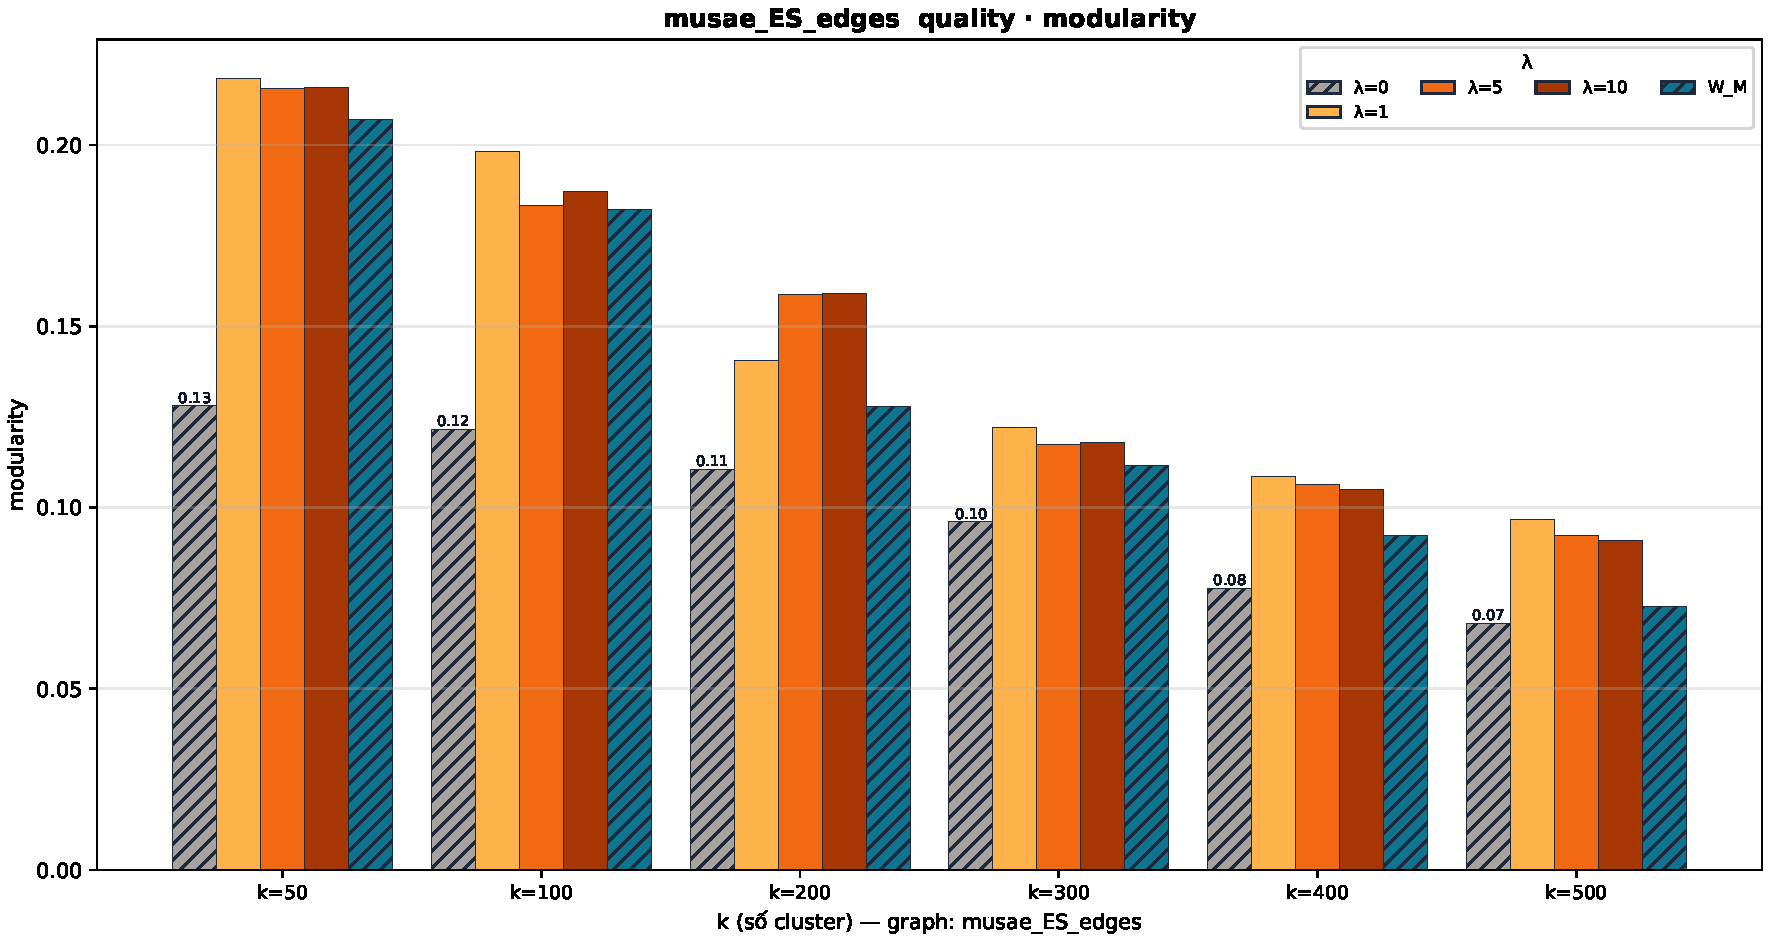
\includegraphics[width=\textwidth]{../main_result/REAL/musae_ES_edges/charts/quality_modularity.pdf}
    \caption{Modularity $Q$ trên musae\_ES theo $\lambda$ và $K$.}
    \label{fig:real-musae-es}
\end{figure}

$Q(0)$ thuộc khoảng $0{,}07$--$0{,}13$, sát chế độ của musae\_DE. Cải thiện lớn nhất tại $K = 50$ với $\Delta Q = +0{,}0902$, tương ứng tăng khoảng $70\%$. $\lambda^* = 1$ ở $K = 50$, nhỏ hơn $W_M$ của musae\_DE, cho thấy đóng góp tối ưu của motif đã đạt ở mức trọng số trung bình.

\textbf{Hệ số phân cụm.}
\begin{figure}[H]
    \centering
    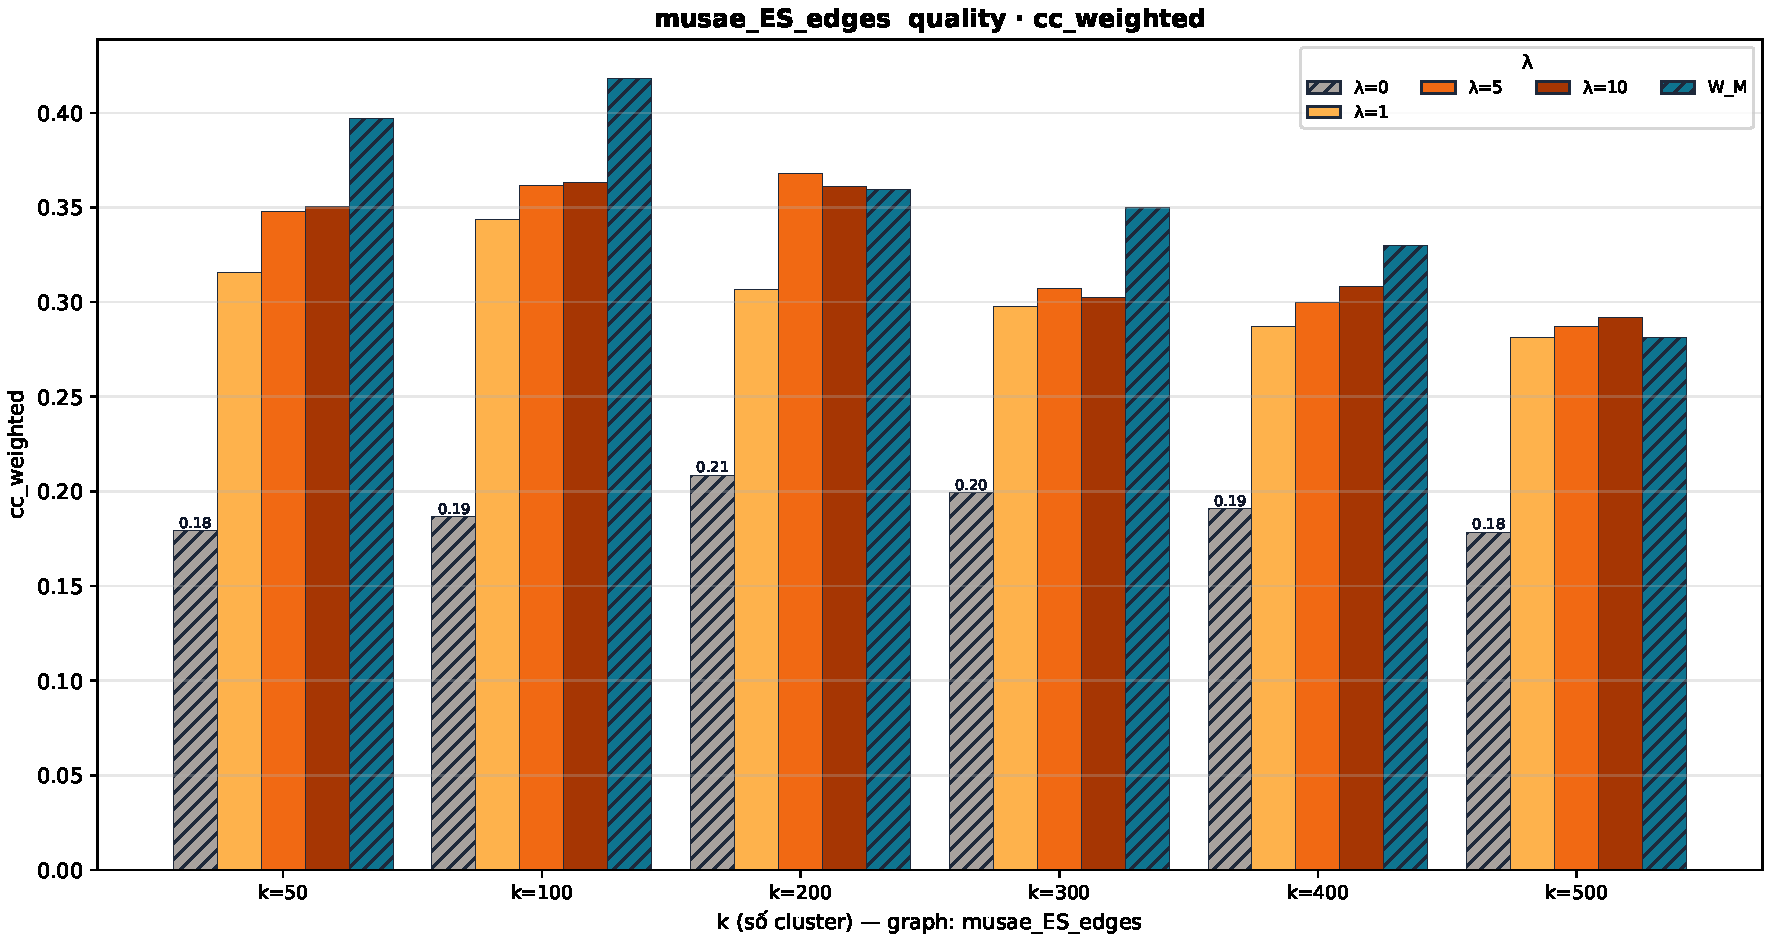
\includegraphics[width=\textwidth]{../main_result/REAL/musae_ES_edges/charts/quality_cc_weighted.pdf}
    \caption{$\overline{\mathrm{CC}}_w$ trên musae\_ES theo $\lambda$ và $K$.}
    \label{fig:real-cc-musae-es}
\end{figure}

\begin{figure}[H]
    \centering
    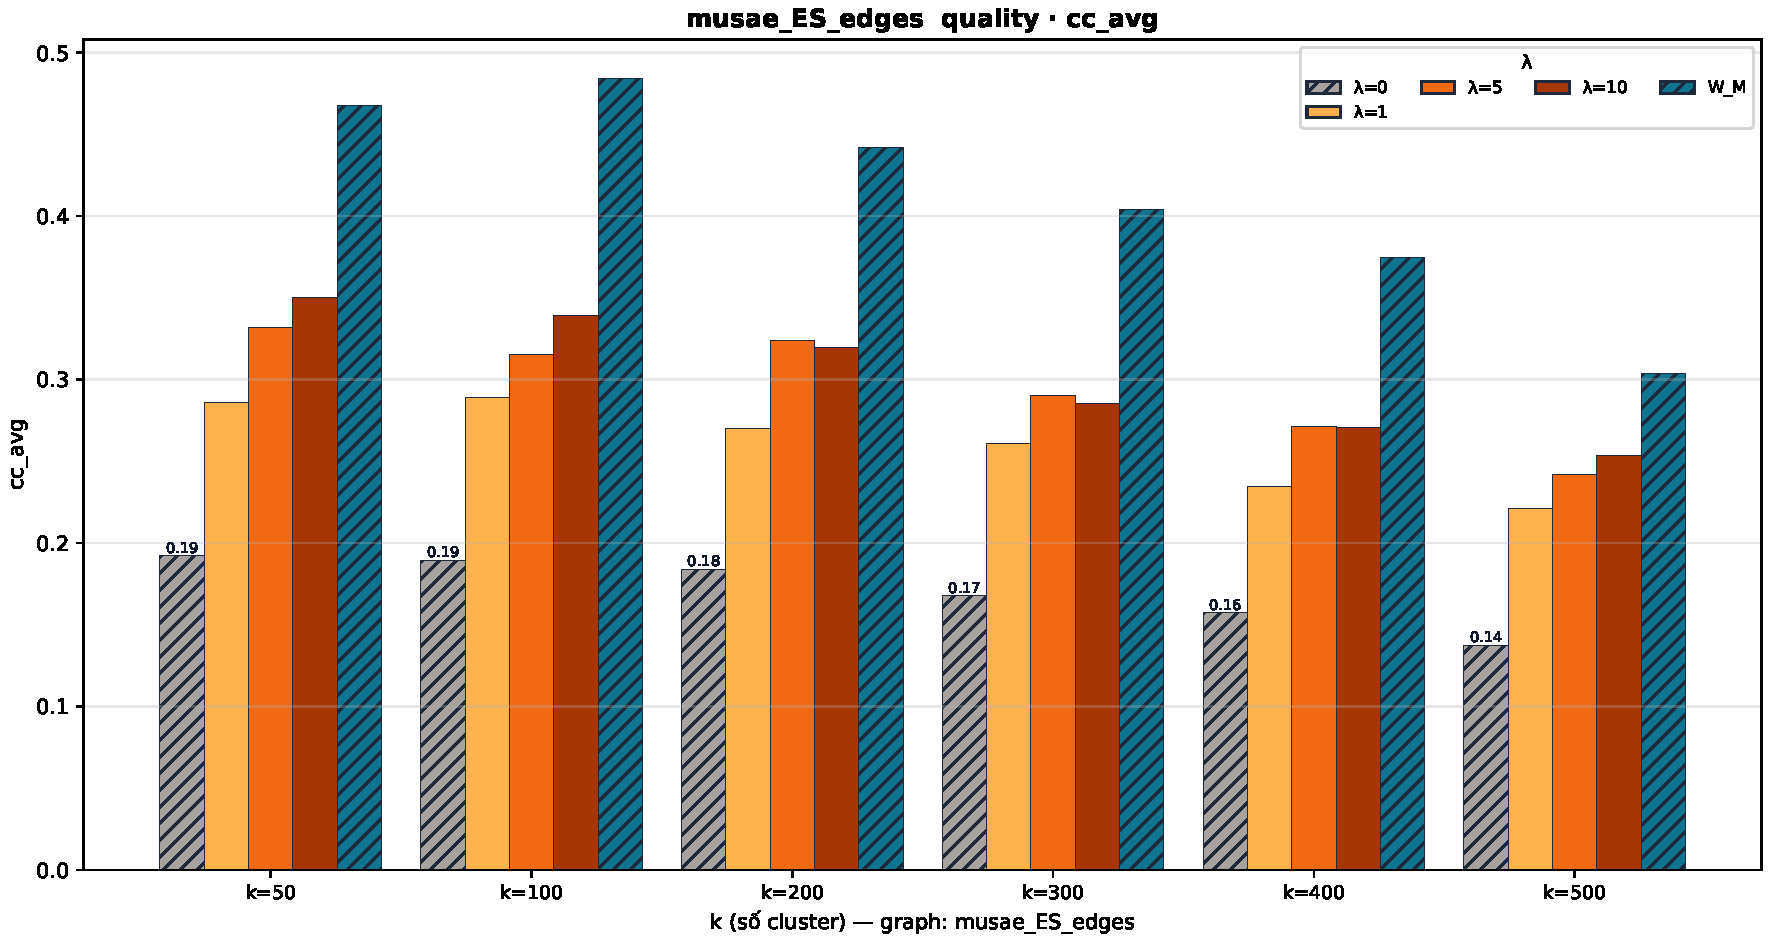
\includegraphics[width=\textwidth]{../main_result/REAL/musae_ES_edges/charts/quality_cc_avg.pdf}
    \caption{$\overline{\mathrm{CC}}$ trên musae\_ES theo $\lambda$ và $K$.}
    \label{fig:real-ccavg-musae-es}
\end{figure}

Tại $K = 50$, $\overline{\mathrm{CC}}_w(0) = 0{,}1793$ vẫn dưới $cc_{\mathrm{global}}$, sau đó tăng lên $0{,}3968$ tại $W_M$, gấp khoảng hai lần. $\overline{\mathrm{CC}}$ bật từ $0{,}3504$ tại $\lambda = 10$ lên $0{,}4678$ tại $W_M$ (tăng $0{,}12$), nhanh hơn rõ rệt so với $\overline{\mathrm{CC}}_w$ (tăng $0{,}05$ trong cùng đoạn). Lặp lại pattern của musae\_DE: $W_M$ tạo nhiều cụm nhỏ thiên lệch $\overline{\mathrm{CC}}$.

\textbf{Kết luận.} Cùng họ với musae\_DE nhưng quy mô nhỏ hơn, musae\_ES tái lập cùng pattern: phân cụm phổ thuần bỏ sót cấu trúc tam giác, trọng số motif khôi phục được tín hiệu cộng đồng. Việc $\lambda^*$ nhỏ hơn (giá trị $1$ thay vì $W_M$) phản ánh quy mô nhỏ làm tín hiệu cạnh đã có đóng góp tương đối, nên không cần trọng số motif cực đại.

% ............................................................
\subsection*{lastfm\_asia}

Đỉnh là một người dùng LastFM ở châu Á, cạnh là quan hệ bạn bè trong nền tảng. Cộng đồng có xu hướng theo quốc gia hoặc sở thích âm nhạc. Hệ số phân cụm toàn cục $cc_{\mathrm{global}} = 0{,}2194$, đồ thị thưa hơn musae.

\textbf{Modularity.}
\begin{figure}[H]
    \centering
    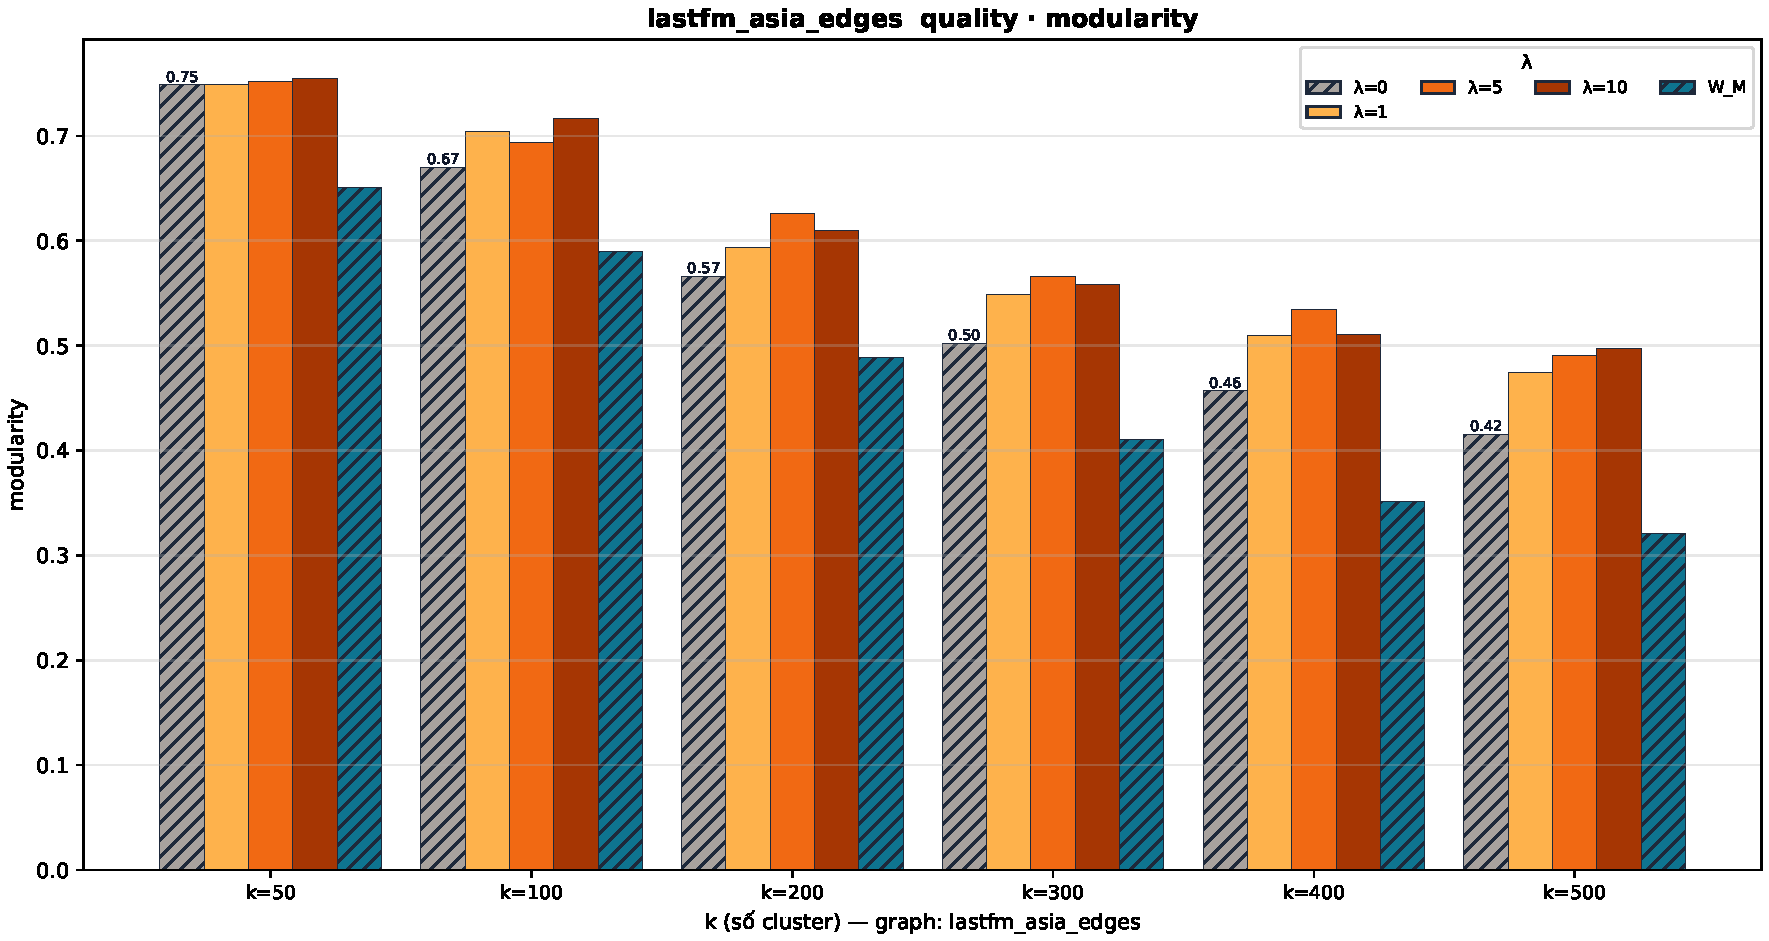
\includegraphics[width=\textwidth]{../main_result/REAL/lastfm_asia_edges/charts/quality_modularity.pdf}
    \caption{Modularity $Q$ trên lastfm\_asia theo $\lambda$ và $K$.}
    \label{fig:real-lastfm}
\end{figure}

Đồ thị này phơi bày cả hai chế độ trên cùng một dataset. Tại $K = 50$, $Q(0) = 0{,}7486$ đã cao và $\Delta Q$ chỉ $+0{,}0059$. Tại $K = 500$, $Q(0)$ tụt còn $0{,}4155$ và $\Delta Q$ vọt lên $+0{,}0815$ với $\lambda^* = 10$. Mức độ cải thiện do trọng số motif tỉ lệ nghịch với chất lượng phân hoạch ban đầu.

\textbf{Hệ số phân cụm.}
\begin{figure}[H]
    \centering
    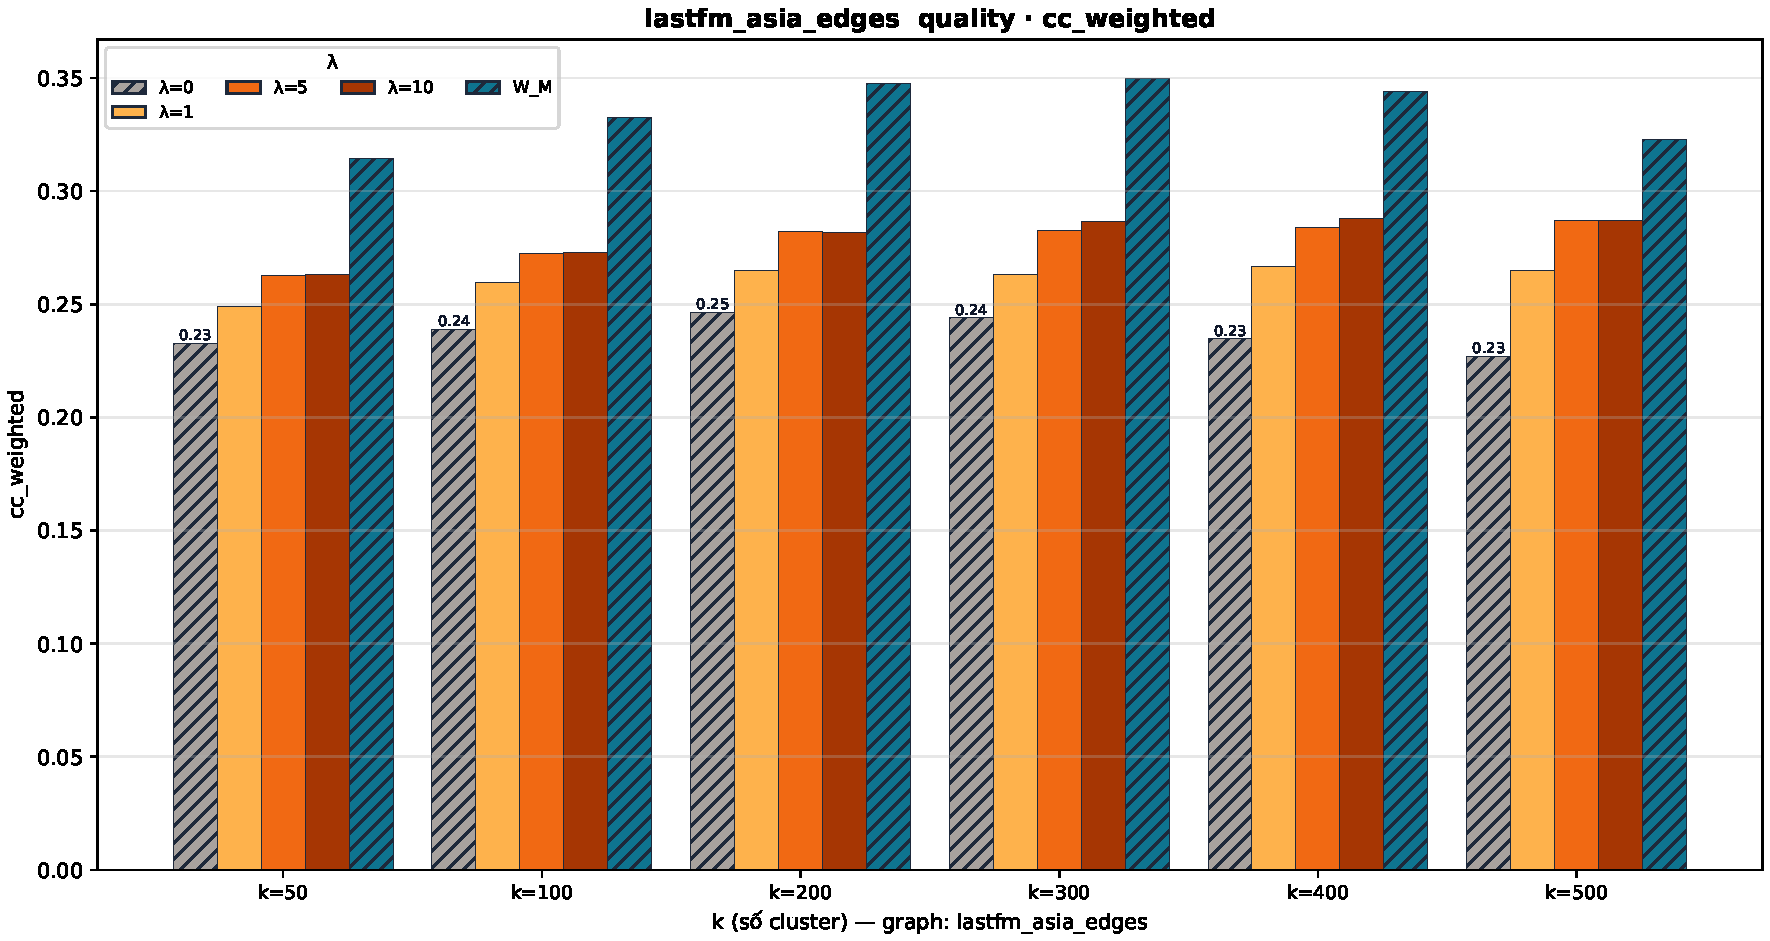
\includegraphics[width=\textwidth]{../main_result/REAL/lastfm_asia_edges/charts/quality_cc_weighted.pdf}
    \caption{$\overline{\mathrm{CC}}_w$ trên lastfm\_asia theo $\lambda$ và $K$.}
    \label{fig:real-cc-lastfm}
\end{figure}

\begin{figure}[H]
    \centering
    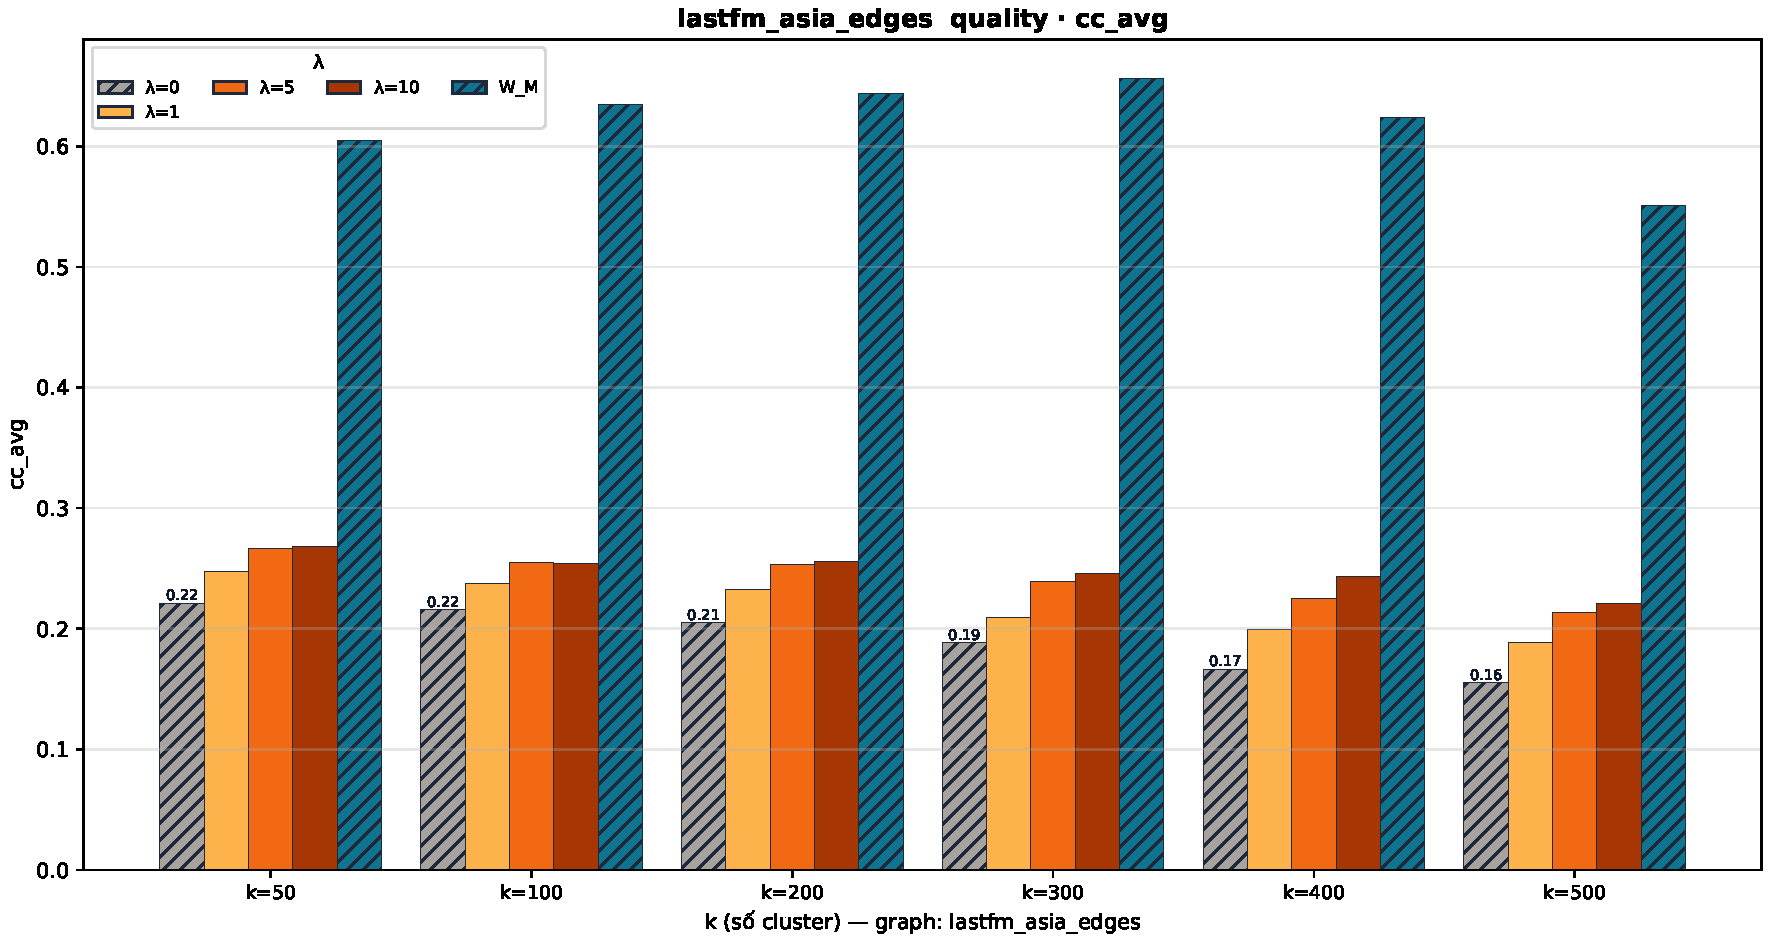
\includegraphics[width=\textwidth]{../main_result/REAL/lastfm_asia_edges/charts/quality_cc_avg.pdf}
    \caption{$\overline{\mathrm{CC}}$ trên lastfm\_asia theo $\lambda$ và $K$.}
    \label{fig:real-ccavg-lastfm}
\end{figure}

Tại $K = 50$, $\overline{\mathrm{CC}}_w(0) = 0{,}2328$ đã gần $cc_{\mathrm{global}}$, tăng lên $0{,}3146$ tại $W_M$. $\overline{\mathrm{CC}}$ tại $W_M$ đạt $0{,}6044$, chênh tới $0{,}29$ so với $\overline{\mathrm{CC}}_w$, lớn nhất trong toàn bộ tập dữ liệu thật; con số này bật từ $0{,}2681$ tại $\lambda = 10$ chỉ qua một bước. Đây là minh hoạ rõ nhất cho hiện tượng phân mảnh cụm khi $\lambda \to \infty$ đã trình bày ở Định nghĩa~\ref{def:cc-cluster}: $W_M$ sinh nhiều cụm rất nhỏ với hệ số phân cụm cục bộ cao, đẩy $\overline{\mathrm{CC}}$ vọt lên trong khi $\overline{\mathrm{CC}}_w$ tiếp tục cho con số thận trọng.

\textbf{Kết luận.} lastfm\_asia là ví dụ điển hình về đồ thị xã hội thưa với cộng đồng đa quy mô. Tại $K$ nhỏ, các cụm lớn đã định hình tốt qua cạnh; tại $K$ lớn, cần bóc tách thêm các nhóm sở thích nhỏ và motif đóng vai trò quan trọng. Chênh lệch lớn giữa $\overline{\mathrm{CC}}$ và $\overline{\mathrm{CC}}_w$ khẳng định lựa chọn $\overline{\mathrm{CC}}_w$ làm chỉ số chính: nếu dùng $\overline{\mathrm{CC}}$, chất lượng phân hoạch trên đồ thị này sẽ bị đánh giá quá lạc quan.

% ............................................................
\subsection*{Email-Enron}

Đỉnh là một địa chỉ email nội bộ công ty Enron, cạnh nếu có ít nhất một thư trao đổi giữa hai địa chỉ. Cộng đồng có nghĩa là phòng ban hoặc nhóm dự án. Hệ số phân cụm toàn cục $cc_{\mathrm{global}} = 0{,}5092$ ở mức cao, phản ánh trao đổi email ba bên trong cùng phòng ban.

\textbf{Modularity.}
\begin{figure}[H]
    \centering
    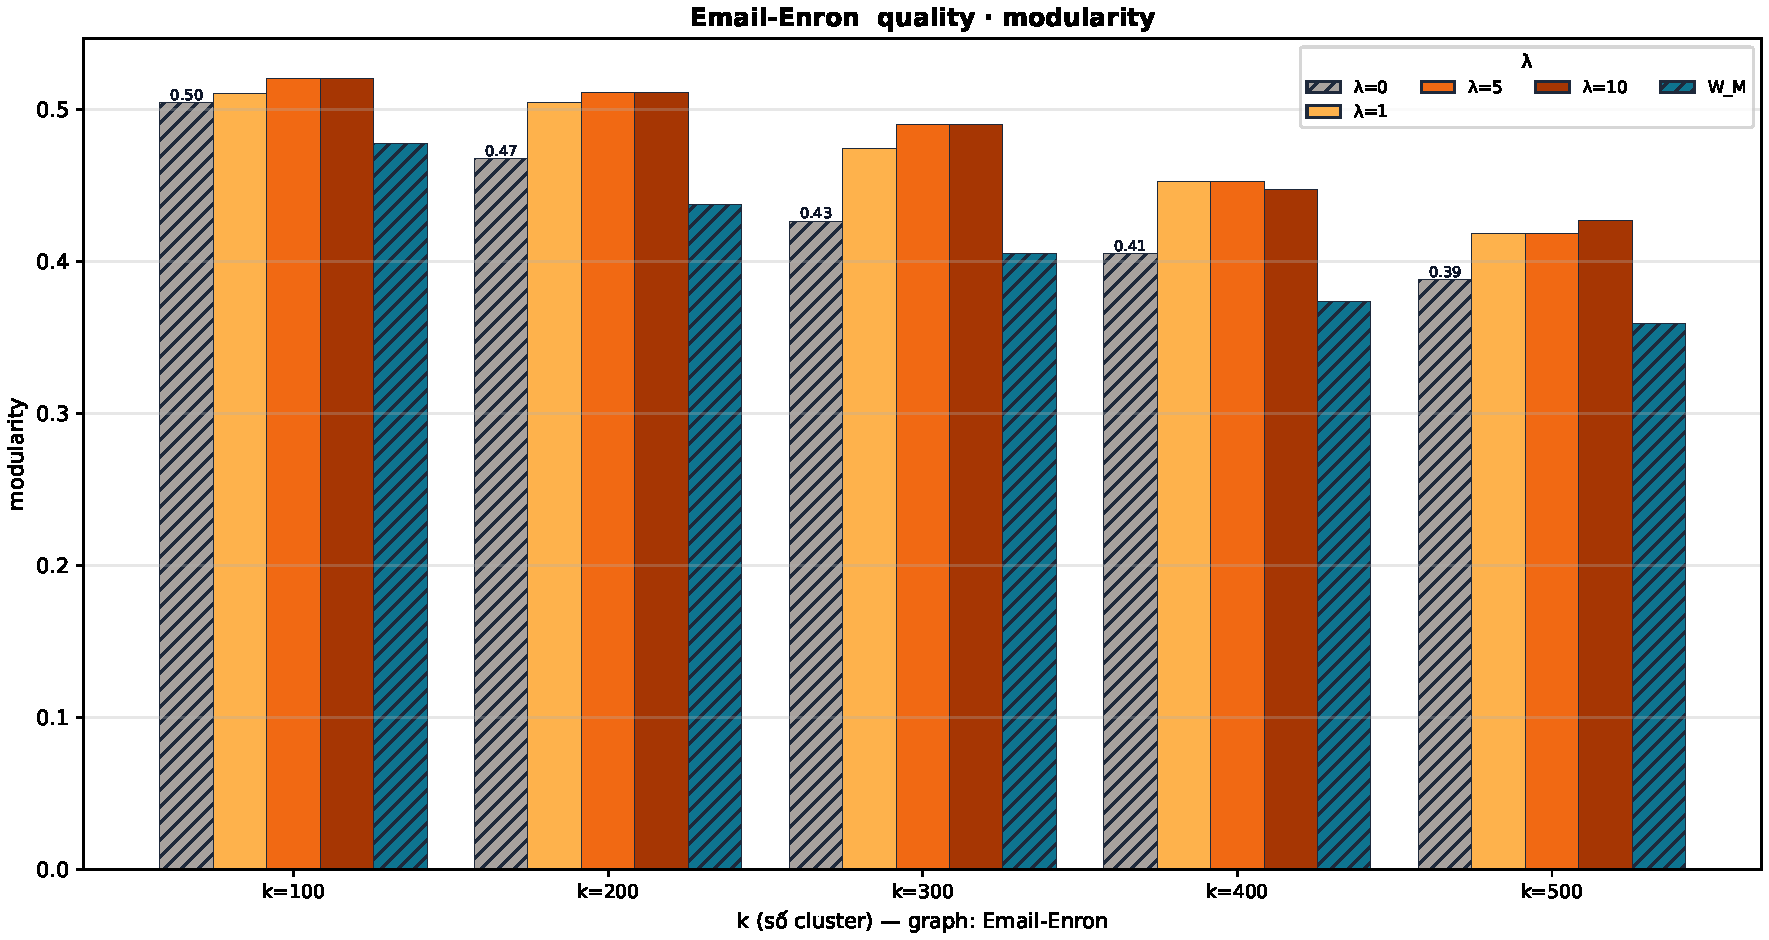
\includegraphics[width=\textwidth]{../main_result/REAL/Email-Enron/charts/quality_modularity.pdf}
    \caption{Modularity $Q$ trên Email-Enron theo $\lambda$ và $K$.}
    \label{fig:real-enron}
\end{figure}

$Q(0)$ thuộc vùng trung gian ($0{,}39$--$0{,}50$). Cải thiện đáng kể trên mọi $K$, $\Delta Q$ dao động từ $+0{,}016$ tại $K = 100$ đến $+0{,}064$ tại $K = 300$, bám sát quy luật $Q(0)$ càng thấp thì $\Delta Q$ càng lớn. Tại $K = 300$, $\lambda^* = 5$.

\textbf{Hệ số phân cụm.}
\begin{figure}[H]
    \centering
    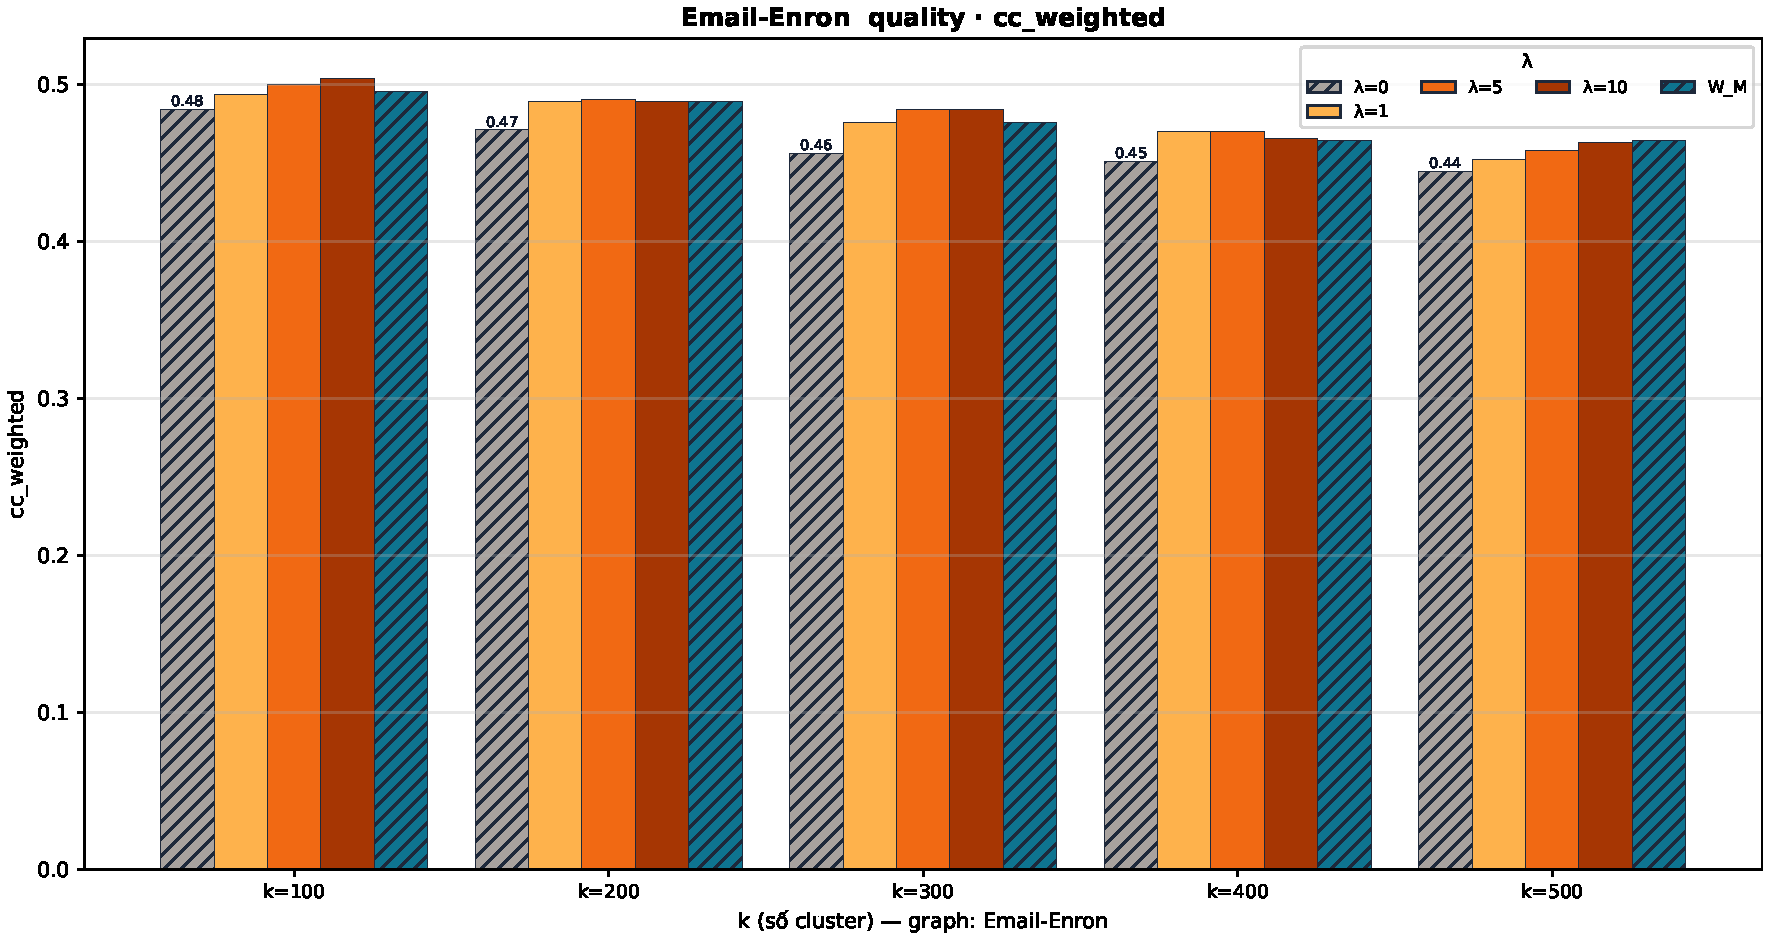
\includegraphics[width=\textwidth]{../main_result/REAL/Email-Enron/charts/quality_cc_weighted.pdf}
    \caption{$\overline{\mathrm{CC}}_w$ trên Email-Enron theo $\lambda$ và $K$.}
    \label{fig:real-cc-enron}
\end{figure}

\begin{figure}[H]
    \centering
    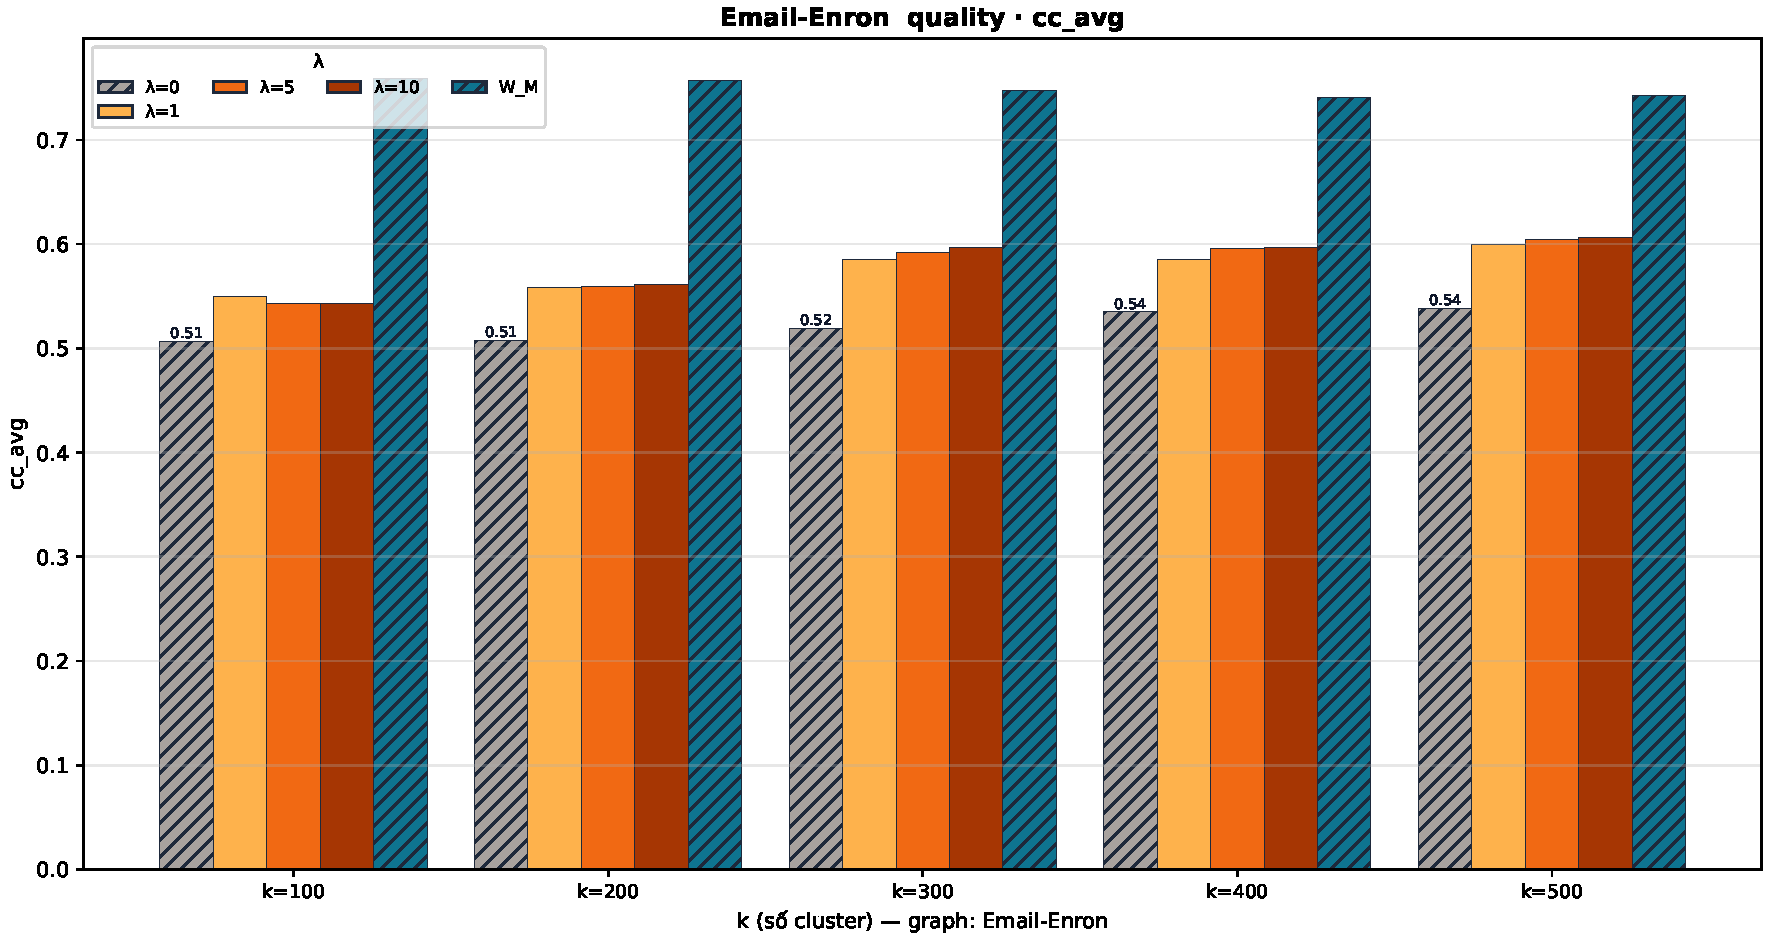
\includegraphics[width=\textwidth]{../main_result/REAL/Email-Enron/charts/quality_cc_avg.pdf}
    \caption{$\overline{\mathrm{CC}}$ trên Email-Enron theo $\lambda$ và $K$.}
    \label{fig:real-ccavg-enron}
\end{figure}

Tại $K = 100$, $\overline{\mathrm{CC}}_w(0) = 0{,}4844$ đã sát $cc_{\mathrm{global}}$. Mức tăng nhẹ lên $0{,}5040$ tại $\lambda = 10$ là biên độ điển hình của đồ thị có $cc_{\mathrm{global}}$ cao. $\overline{\mathrm{CC}}$ tại $\lambda = 10$ chênh $0{,}04$ so với $\overline{\mathrm{CC}}_w$ ($0{,}5432$ so với $0{,}5040$), nhưng tại $W_M$ bật lên $0{,}7592$ trong khi $\overline{\mathrm{CC}}_w$ tụt còn $0{,}4959$, mở rộng chênh lệch lên $0{,}26$. Đây là một trong những trường hợp $W_M$ làm phân mảnh cụm rõ nhất, được $\overline{\mathrm{CC}}_w$ phát hiện và phạt đúng.

\textbf{Kết luận.} Email-Enron thuộc nhóm đồ thị có cấu trúc tam giác đã được phân cụm phổ trên $A$ khai thác tốt, khoảng cải thiện CC còn lại cho $W_\lambda$ tương đối hẹp. Tuy nhiên modularity vẫn cải thiện đáng kể, cho thấy motif giúp tinh chỉnh ranh giới cụm chứ không tạo ra cấu trúc tam giác mới.

% ............................................................
\subsection*{facebook\_combined}

Hợp của mười ego-network: với mỗi trong mười người dùng Facebook, ta lấy đồ thị bạn bè của họ rồi ghép lại. Đỉnh là người dùng, cạnh là quan hệ bạn bè. Cộng đồng có nghĩa là vòng quan hệ xã hội của từng ego. Hệ số phân cụm toàn cục $cc_{\mathrm{global}} = 0{,}6055$ rất cao, đặc trưng của cấu trúc ego-network.

\textbf{Modularity.}
\begin{figure}[H]
    \centering
    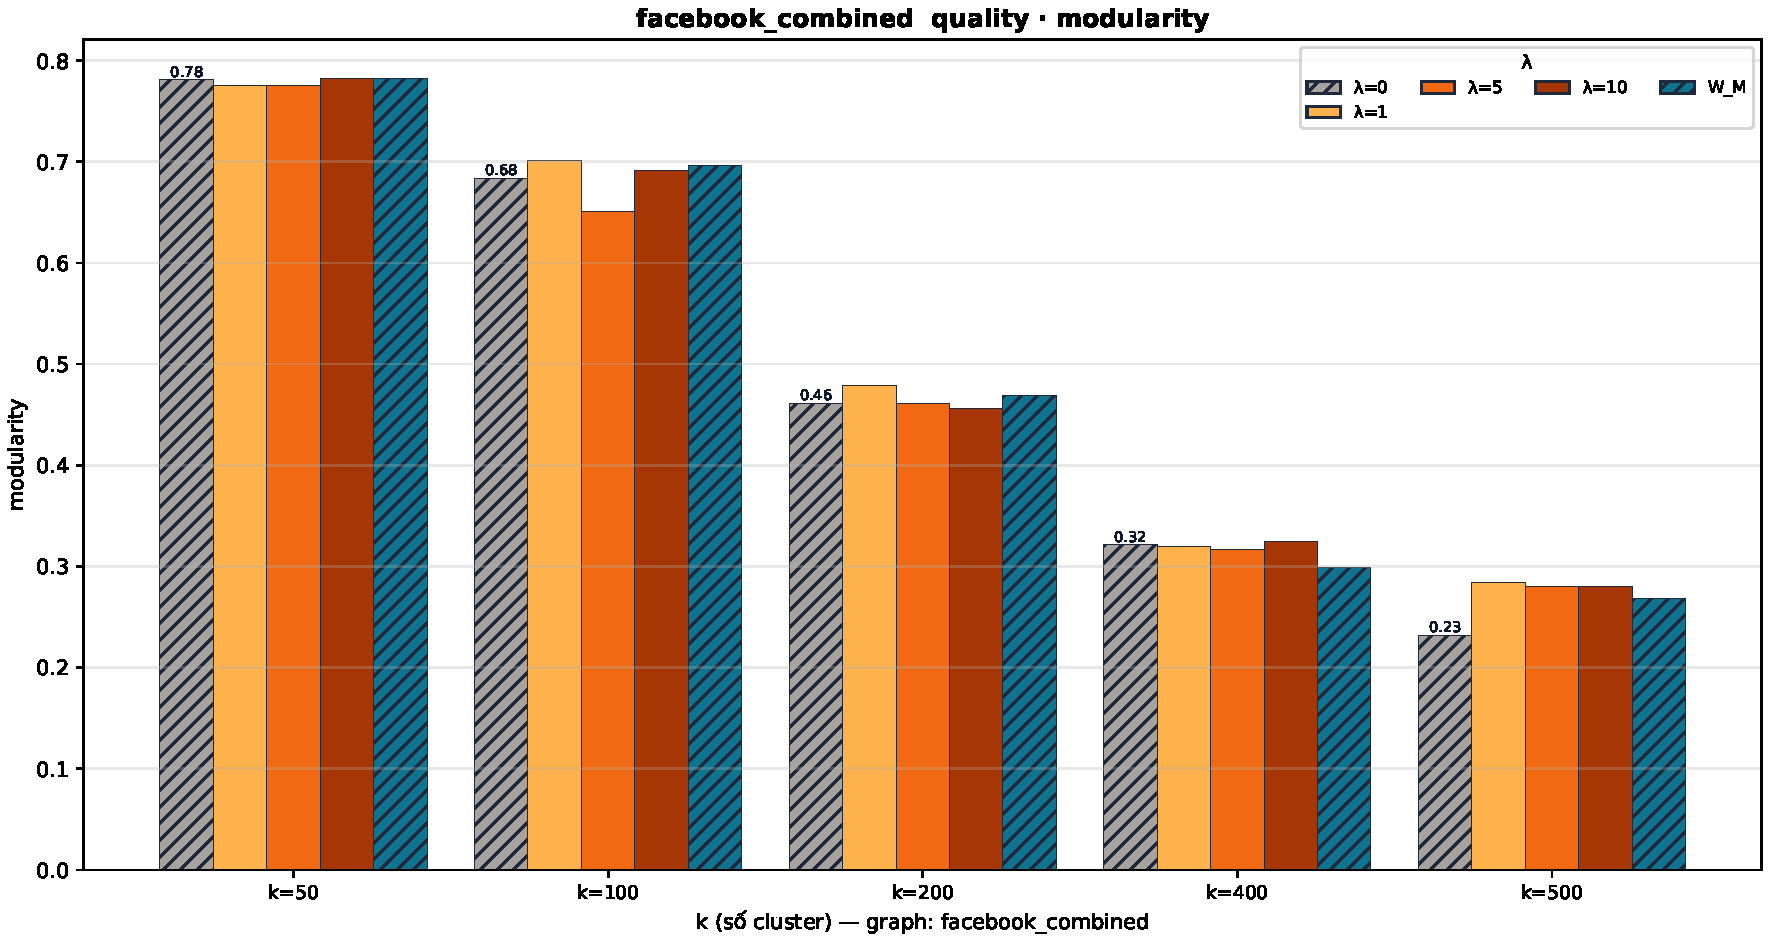
\includegraphics[width=\textwidth]{../main_result/REAL/facebook_combined/charts/quality_modularity.pdf}
    \caption{Modularity $Q$ trên facebook\_combined theo $\lambda$ và $K$.}
    \label{fig:real-facebook}
\end{figure}

Tại $K = 50$, $Q(0) = 0{,}7810$ rất cao và $\Delta Q = +0{,}0010$ không đáng kể. Khi tăng $K$ lên $500$, $Q(0)$ tụt còn $0{,}2319$ và $\Delta Q$ đạt $+0{,}0519$ với $\lambda^* = 5$. Cùng đồ thị nhưng hai chế độ tách biệt theo $K$.

\textbf{Hệ số phân cụm.}
\begin{figure}[H]
    \centering
    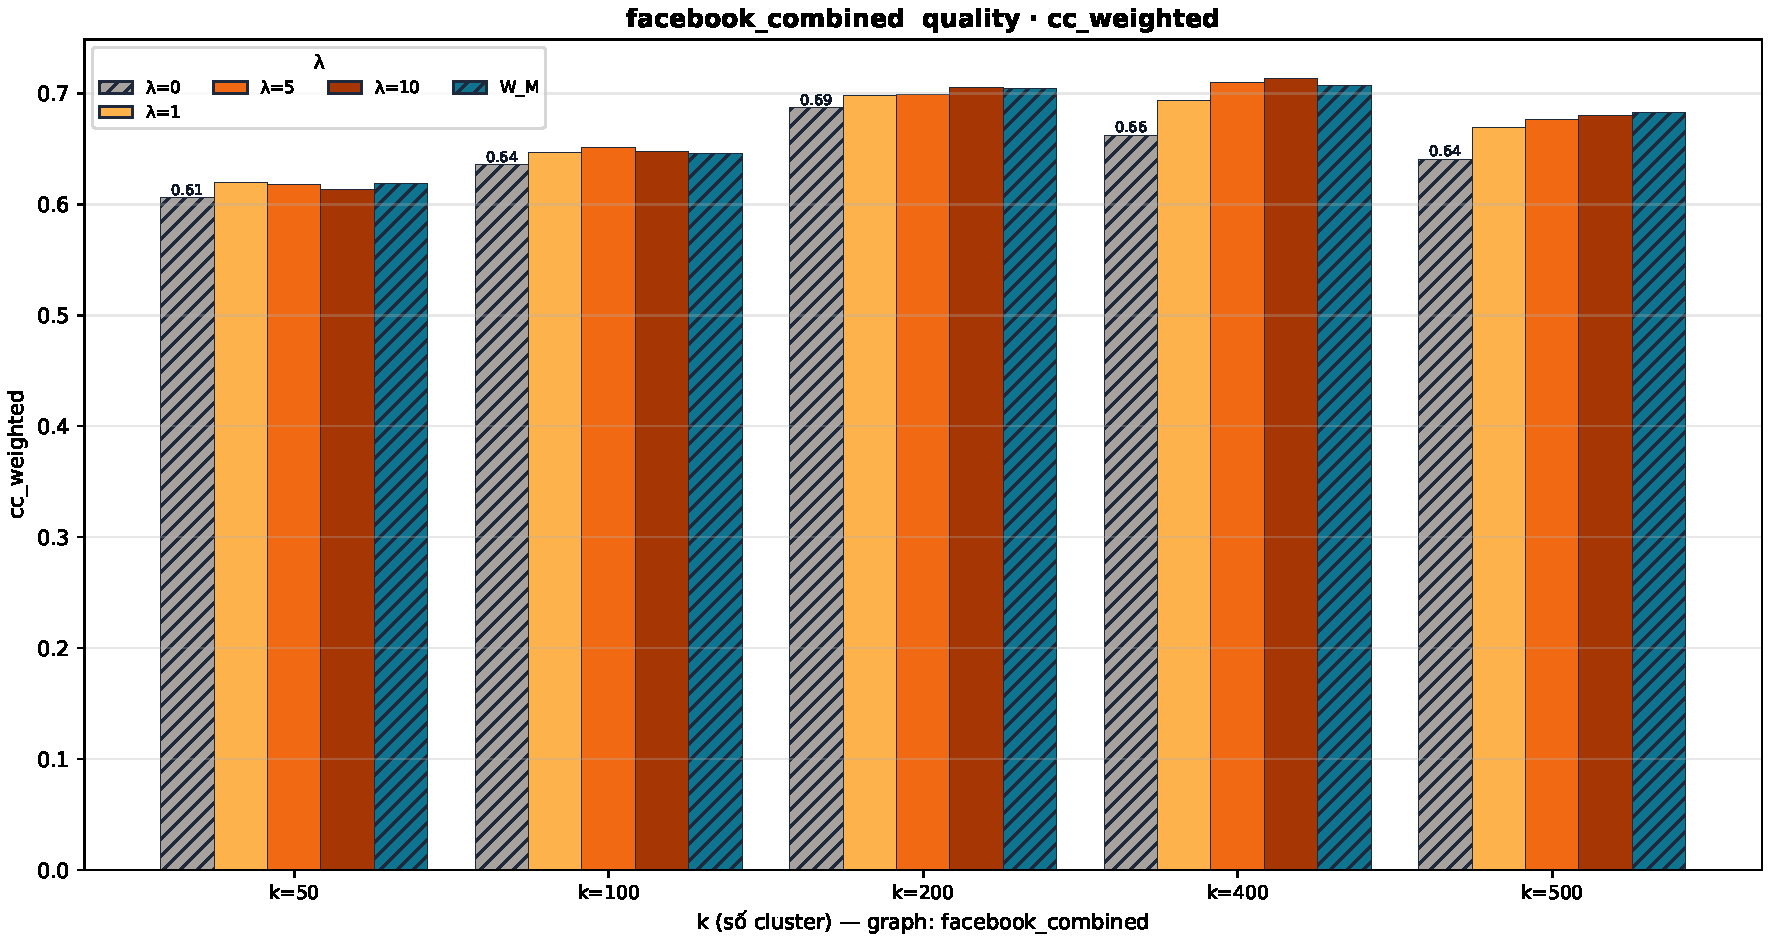
\includegraphics[width=\textwidth]{../main_result/REAL/facebook_combined/charts/quality_cc_weighted.pdf}
    \caption{$\overline{\mathrm{CC}}_w$ trên facebook\_combined theo $\lambda$ và $K$.}
    \label{fig:real-cc-facebook}
\end{figure}

\begin{figure}[H]
    \centering
    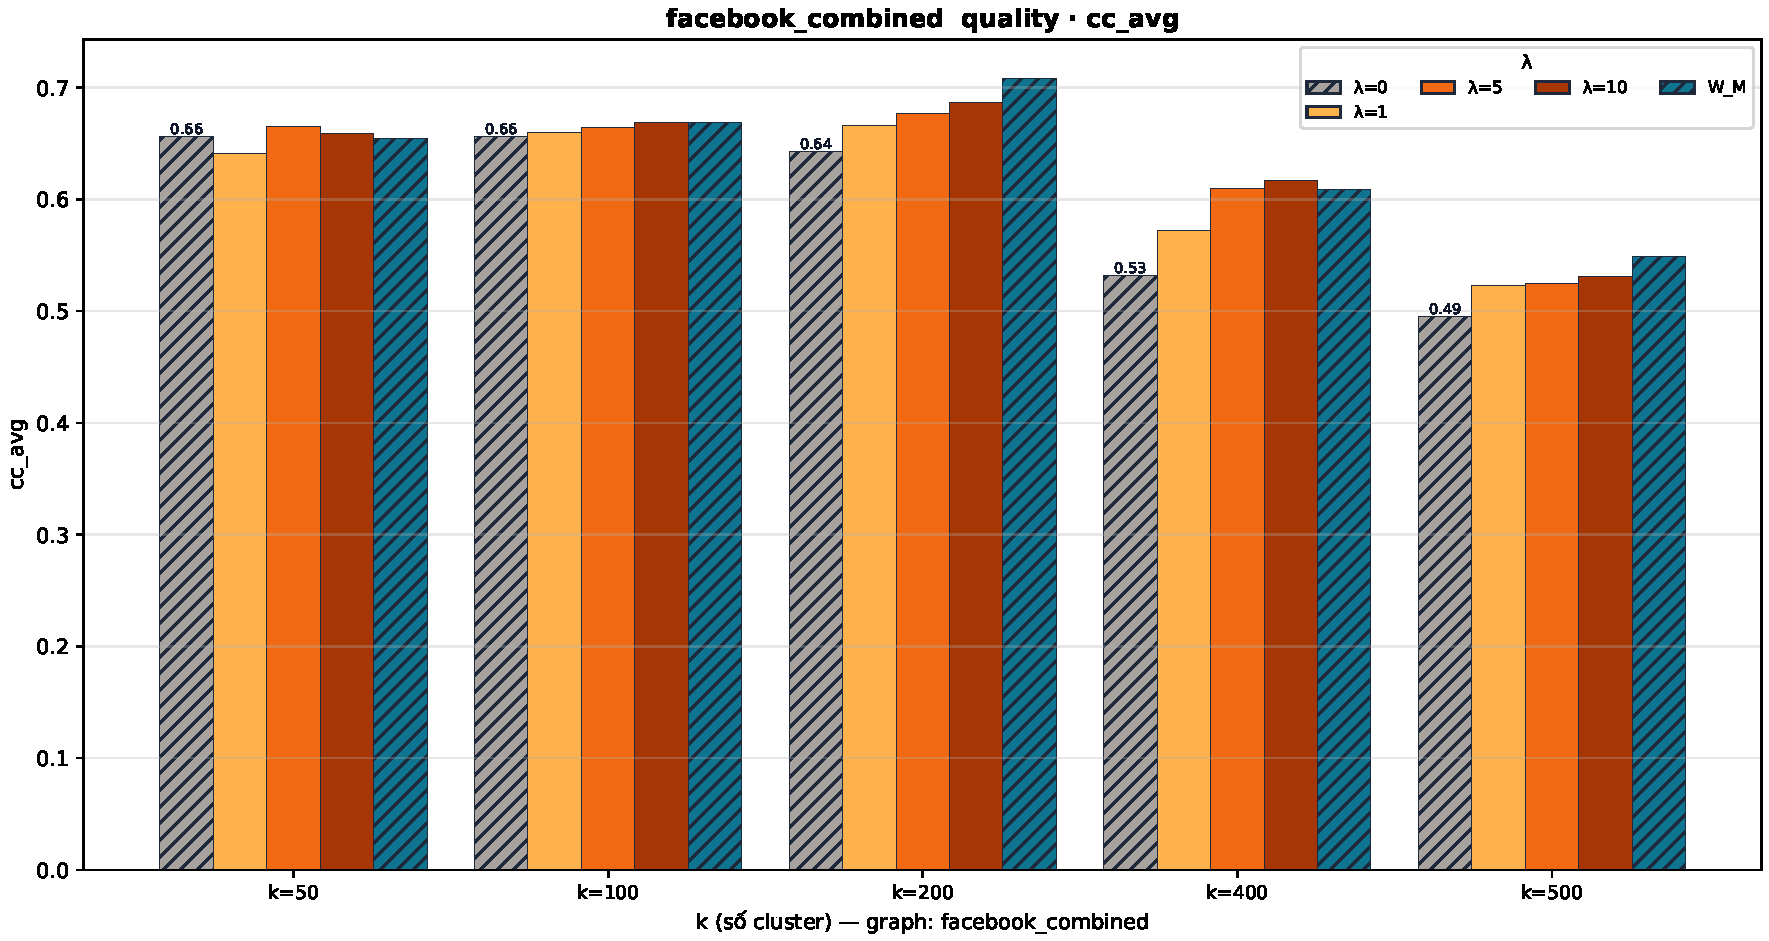
\includegraphics[width=\textwidth]{../main_result/REAL/facebook_combined/charts/quality_cc_avg.pdf}
    \caption{$\overline{\mathrm{CC}}$ trên facebook\_combined theo $\lambda$ và $K$.}
    \label{fig:real-ccavg-facebook}
\end{figure}

Tại $K = 50$, $\overline{\mathrm{CC}}_w(0) = 0{,}6061$ trùng khớp với $cc_{\mathrm{global}}$. Mức tăng theo $\lambda$ rất nhỏ, đạt $0{,}6192$ tại $\lambda = 1$. Khác biệt với phần lớn đồ thị thật, $\overline{\mathrm{CC}}$ tại $W_M$ không bật lên mạnh ($0{,}6548$, gần với giá trị tại $\lambda = 10$ là $0{,}6587$); $\overline{\mathrm{CC}}_w$ cùng giữ ổn định. Cấu trúc ego-network bền vững khiến phân hoạch không bị phân mảnh ngay cả khi bỏ ma trận kề.

\textbf{Kết luận.} facebook\_combined là đồ thị ego-network với cấu trúc tam giác đã trùng khớp gần như hoàn hảo với cộng đồng vòng bạn bè. Khi $K$ nhỏ, mỗi ego tạo thành một cụm tự nhiên và phân cụm phổ trên $A$ đã đạt gần tối đa; vai trò của $W_\lambda$ chỉ rõ rệt khi tăng $K$ để chia tiếp các vòng bạn bè con bên trong mỗi ego.

% ............................................................
\subsection*{CA-GrQc}

Mạng đồng tác giả trên arXiv lĩnh vực Tương đối tổng quát. Đỉnh là một tác giả, cạnh nếu hai tác giả cùng đứng tên trên ít nhất một bài báo. Cộng đồng có nghĩa là nhóm nghiên cứu thường xuyên hợp tác. Hệ số phân cụm toàn cục $cc_{\mathrm{global}} = 0{,}5569$, do bài báo nhiều tác giả tự nhiên sinh tam giác đầy đủ giữa đồng tác giả.

\textbf{Modularity.}
\begin{figure}[H]
    \centering
    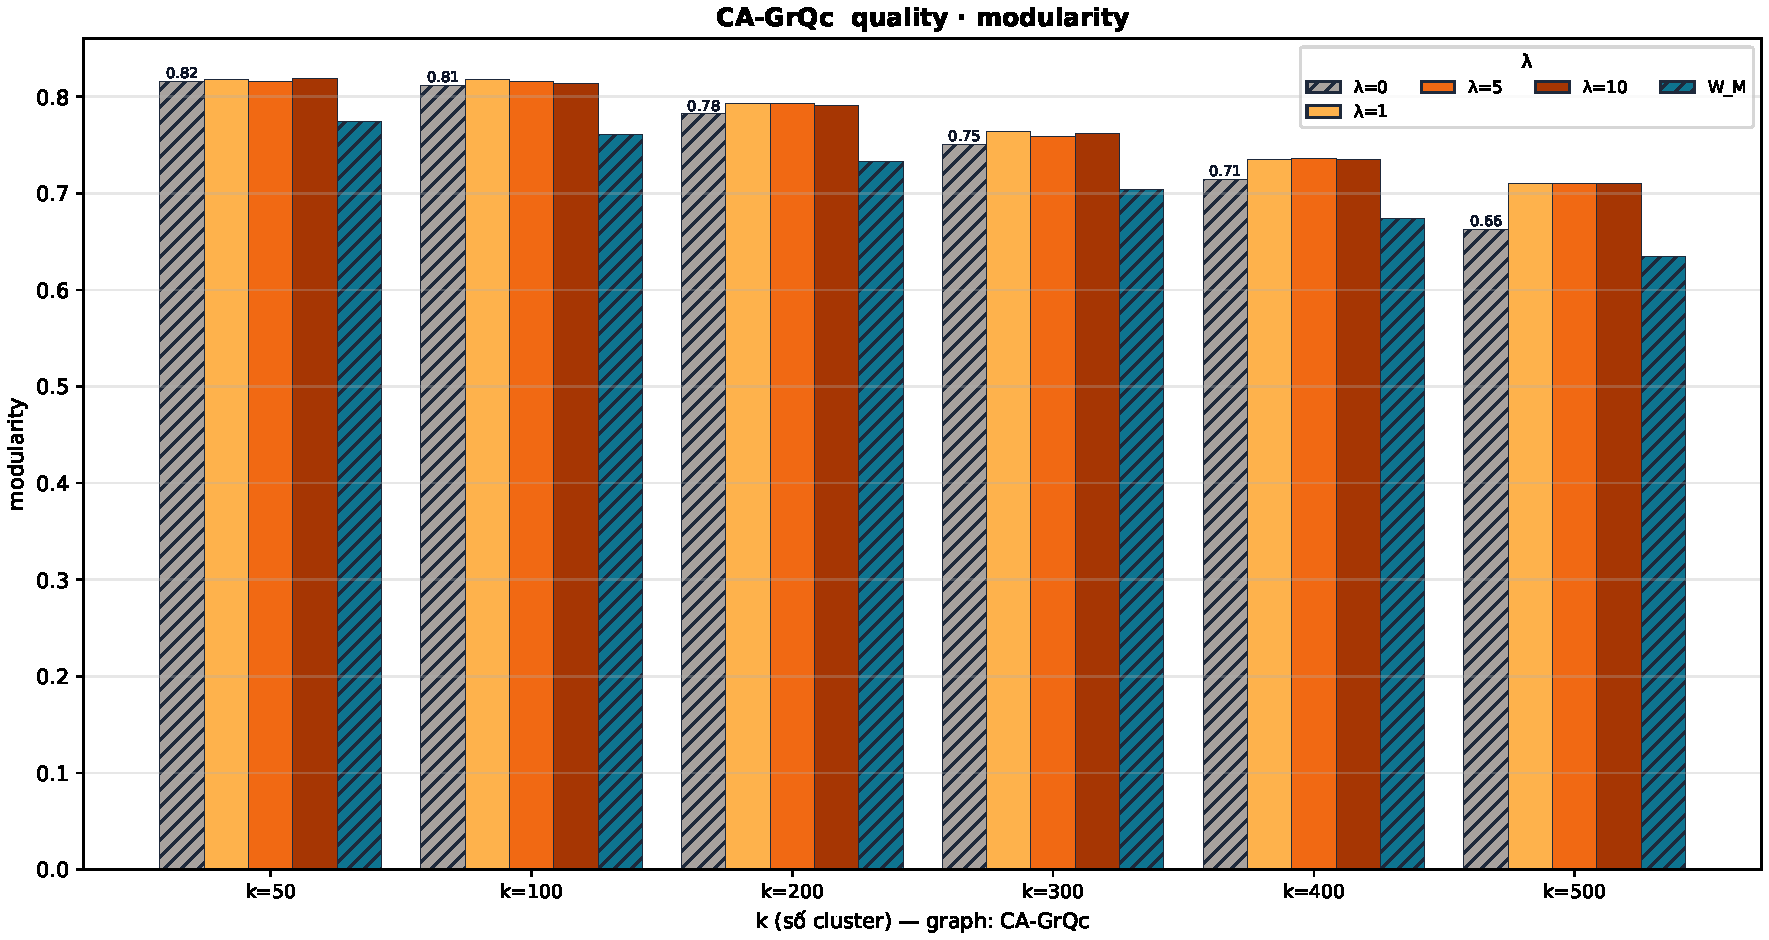
\includegraphics[width=\textwidth]{../main_result/REAL/CA-GrQc/charts/quality_modularity.pdf}
    \caption{Modularity $Q$ trên CA-GrQc theo $\lambda$ và $K$.}
    \label{fig:real-grqc}
\end{figure}

$Q(0)$ cao trên dải rộng ($0{,}66$--$0{,}82$). Tại $K = 50$, $Q(0) = 0{,}8161$ và $\Delta Q = +0{,}0031$ không đáng kể. Chỉ ở $K = 500$ với $Q(0) = 0{,}6630$ thấp hơn, $\Delta Q$ mới đạt $+0{,}0476$ với $\lambda^* = 5$. Phân hoạch chất lượng cao gần như không hưởng lợi từ ma trận hỗn hợp.

\textbf{Hệ số phân cụm.}
\begin{figure}[H]
    \centering
    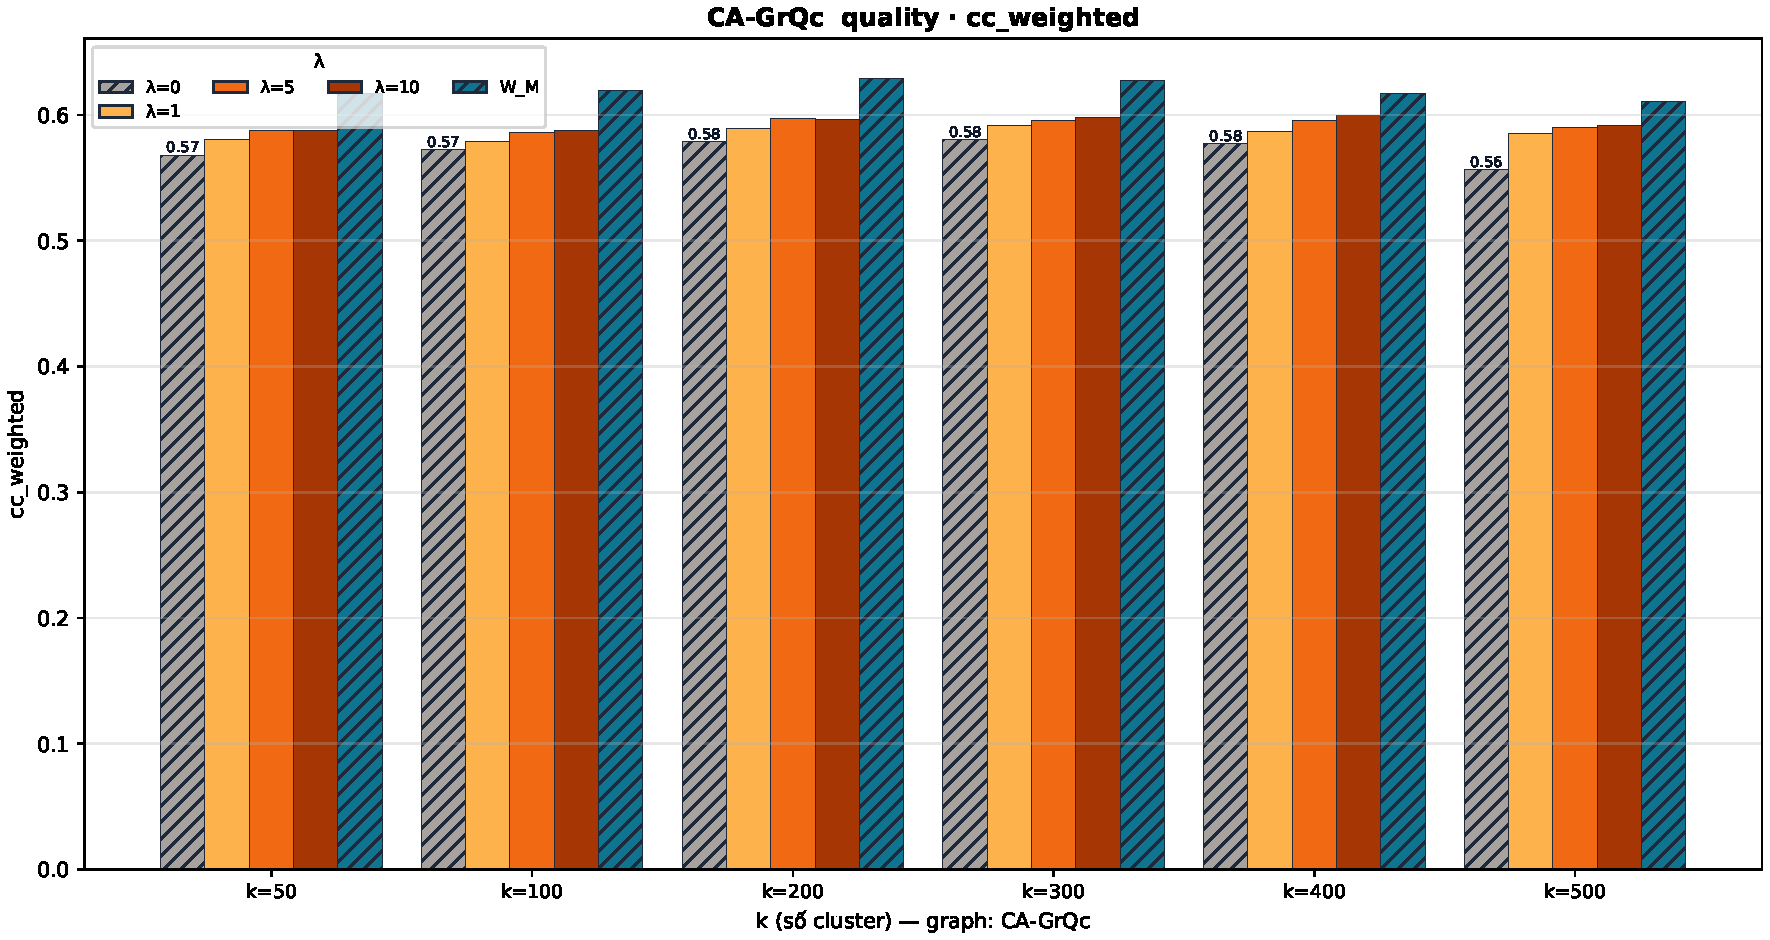
\includegraphics[width=\textwidth]{../main_result/REAL/CA-GrQc/charts/quality_cc_weighted.pdf}
    \caption{$\overline{\mathrm{CC}}_w$ trên CA-GrQc theo $\lambda$ và $K$.}
    \label{fig:real-cc-grqc}
\end{figure}

\begin{figure}[H]
    \centering
    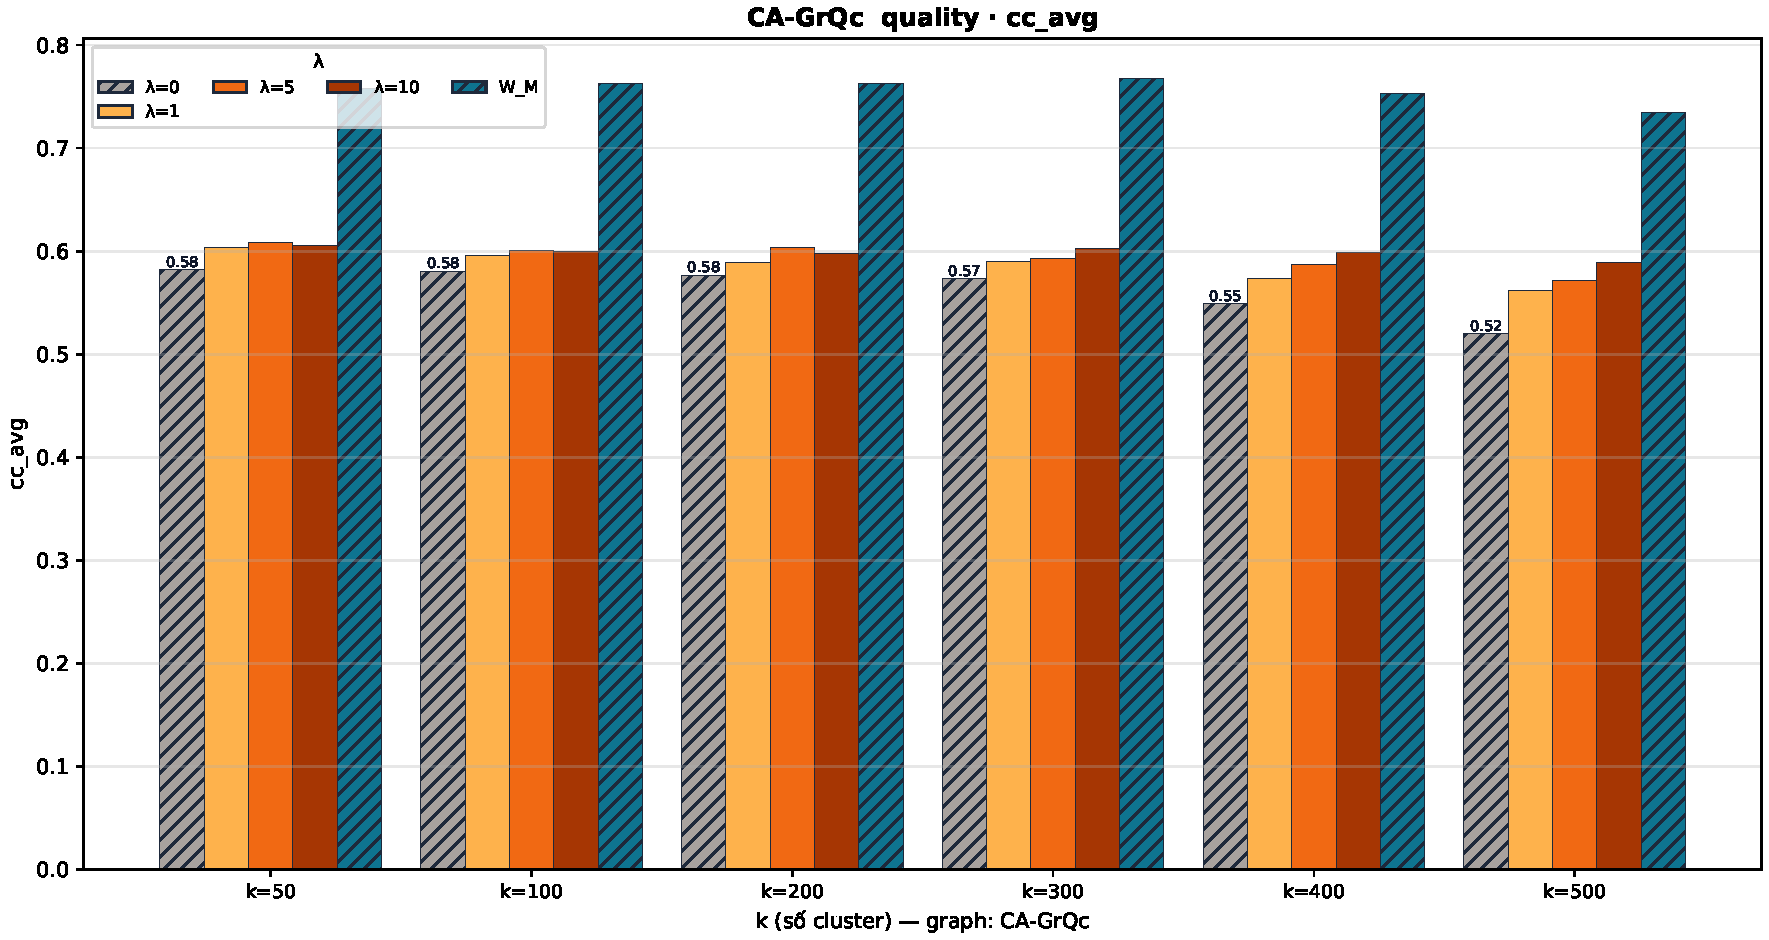
\includegraphics[width=\textwidth]{../main_result/REAL/CA-GrQc/charts/quality_cc_avg.pdf}
    \caption{$\overline{\mathrm{CC}}$ trên CA-GrQc theo $\lambda$ và $K$.}
    \label{fig:real-ccavg-grqc}
\end{figure}

Tại $K = 50$, $\overline{\mathrm{CC}}_w(0) = 0{,}5677$ sát $cc_{\mathrm{global}}$. $\overline{\mathrm{CC}}_w$ tăng nhẹ lên $0{,}6167$ tại $W_M$, biên độ điển hình của đồ thị có $cc_{\mathrm{global}}$ cao. $\overline{\mathrm{CC}}$ bật từ $0{,}6056$ tại $\lambda = 10$ lên $0{,}7574$ tại $W_M$, một bước nhảy $0{,}15$ trong khi $\overline{\mathrm{CC}}_w$ trong cùng đoạn chỉ tăng $0{,}03$. Nhóm nghiên cứu nhỏ với hệ số phân cụm gần $1$ bị $W_M$ tách ra thành cụm riêng, thiên lệch $\overline{\mathrm{CC}}$ nhưng được $\overline{\mathrm{CC}}_w$ giữ ổn định.

\textbf{Kết luận.} CA-GrQc đại diện cho mạng đồng tác giả nhỏ với cấu trúc nhóm nghiên cứu đã được phân cụm phổ trên $A$ phát hiện gần như tối ưu. Vai trò của $W_\lambda$ chỉ thể hiện khi tăng $K$ để chia nhỏ các nhóm lớn; ngược lại, cấu trúc tam giác nội cụm là đặc trưng cố hữu của đồ thị nên $\overline{\mathrm{CC}}_w$ chỉ tăng khiêm tốn.

% ............................................................
\subsection*{CA-AstroPh}

Tương tự CA-GrQc nhưng cho lĩnh vực Vật lý thiên văn. Đồ thị lớn hơn ($n = 17{,}903$) và đậm đặc tam giác hơn. Hệ số phân cụm toàn cục $cc_{\mathrm{global}} = 0{,}6328$ cao hơn CA-GrQc, do cộng tác trong vật lý thiên văn thường nhiều tác giả cùng một bài.

\textbf{Modularity.}
\begin{figure}[H]
    \centering
    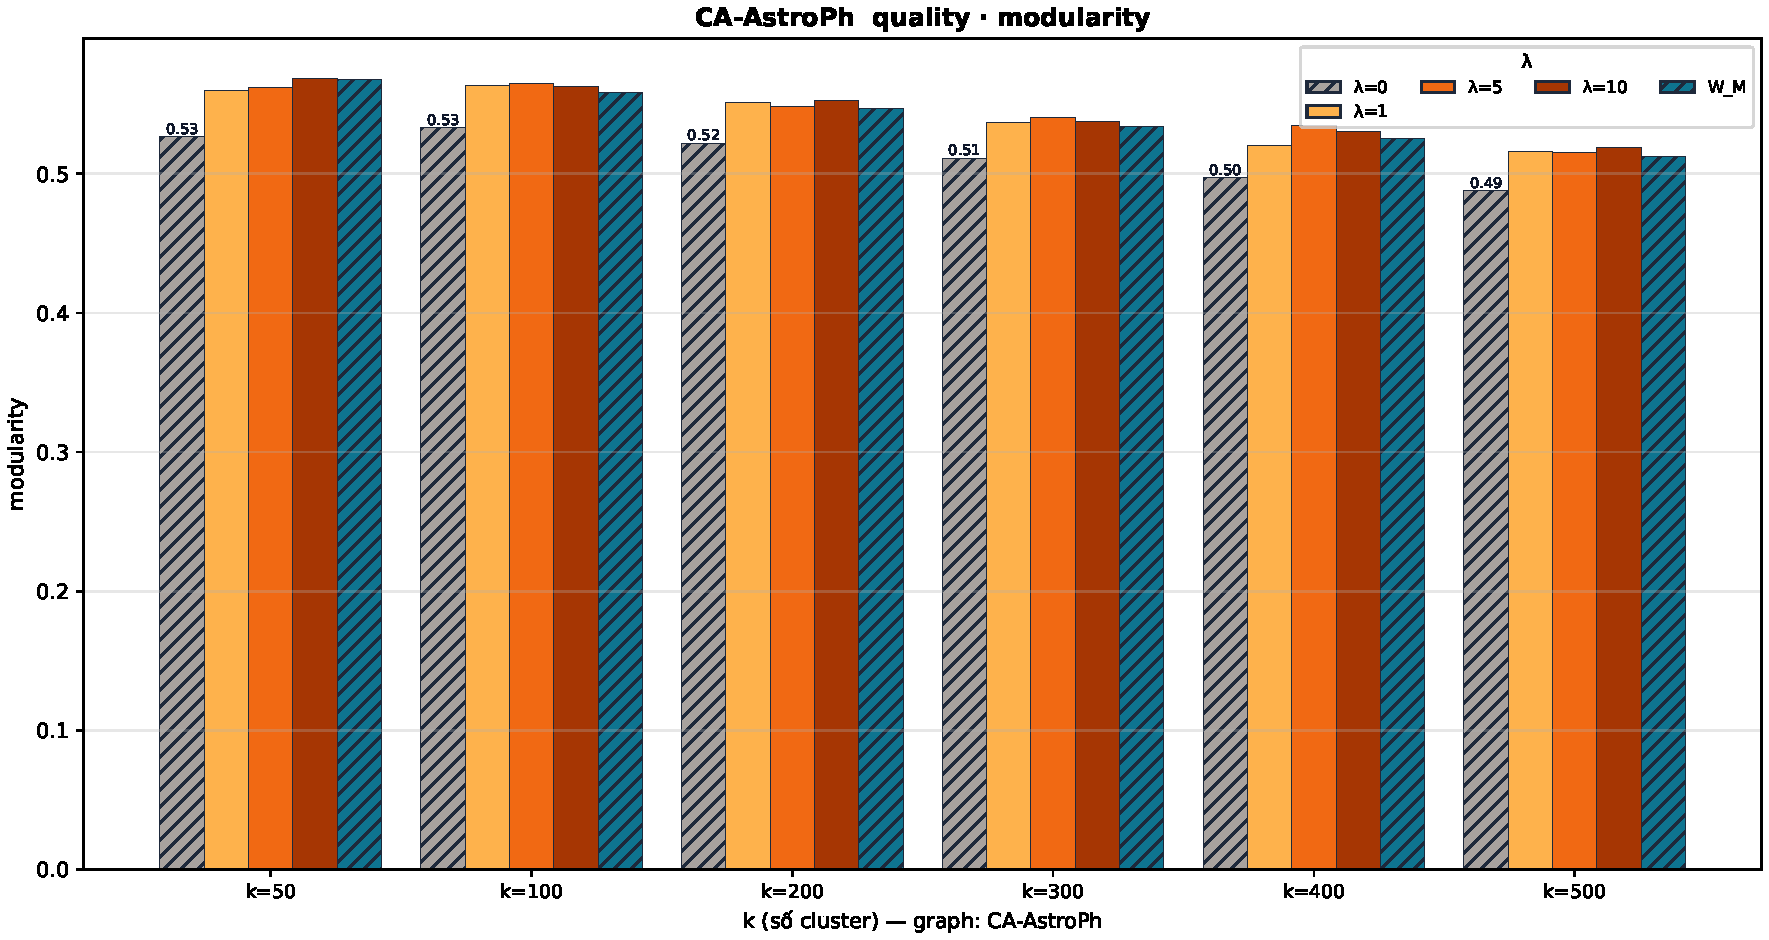
\includegraphics[width=\textwidth]{../main_result/REAL/CA-AstroPh/charts/quality_modularity.pdf}
    \caption{Modularity $Q$ trên CA-AstroPh theo $\lambda$ và $K$.}
    \label{fig:real-astroph}
\end{figure}

$Q(0)$ tập trung ở vùng $0{,}49$--$0{,}53$, cải thiện đồng đều $+0{,}030$ đến $+0{,}042$. Tại $K = 50$, $\Delta Q = +0{,}0421$ với $\lambda^* = 10$. Đồ thị không có bộ test nào ở vùng $Q(0)$ cao nên biên độ $\Delta Q$ không bị thu hẹp như CA-GrQc.

\textbf{Hệ số phân cụm.}
\begin{figure}[H]
    \centering
    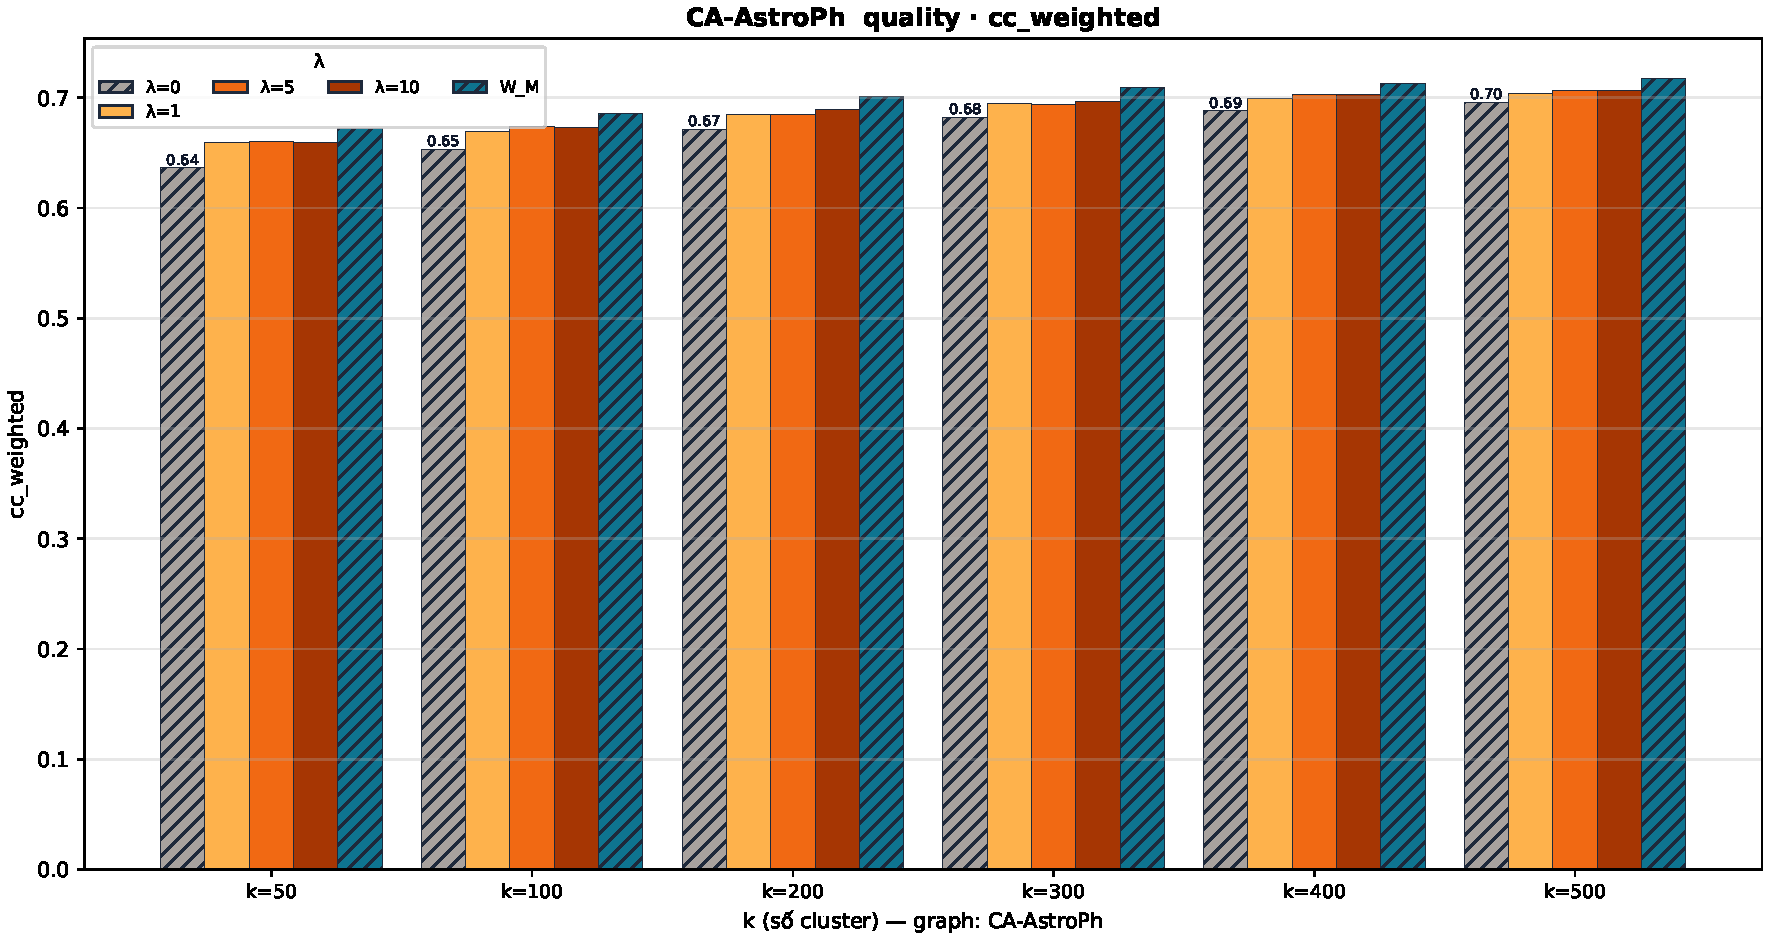
\includegraphics[width=\textwidth]{../main_result/REAL/CA-AstroPh/charts/quality_cc_weighted.pdf}
    \caption{$\overline{\mathrm{CC}}_w$ trên CA-AstroPh theo $\lambda$ và $K$.}
    \label{fig:real-cc-astroph}
\end{figure}

\begin{figure}[H]
    \centering
    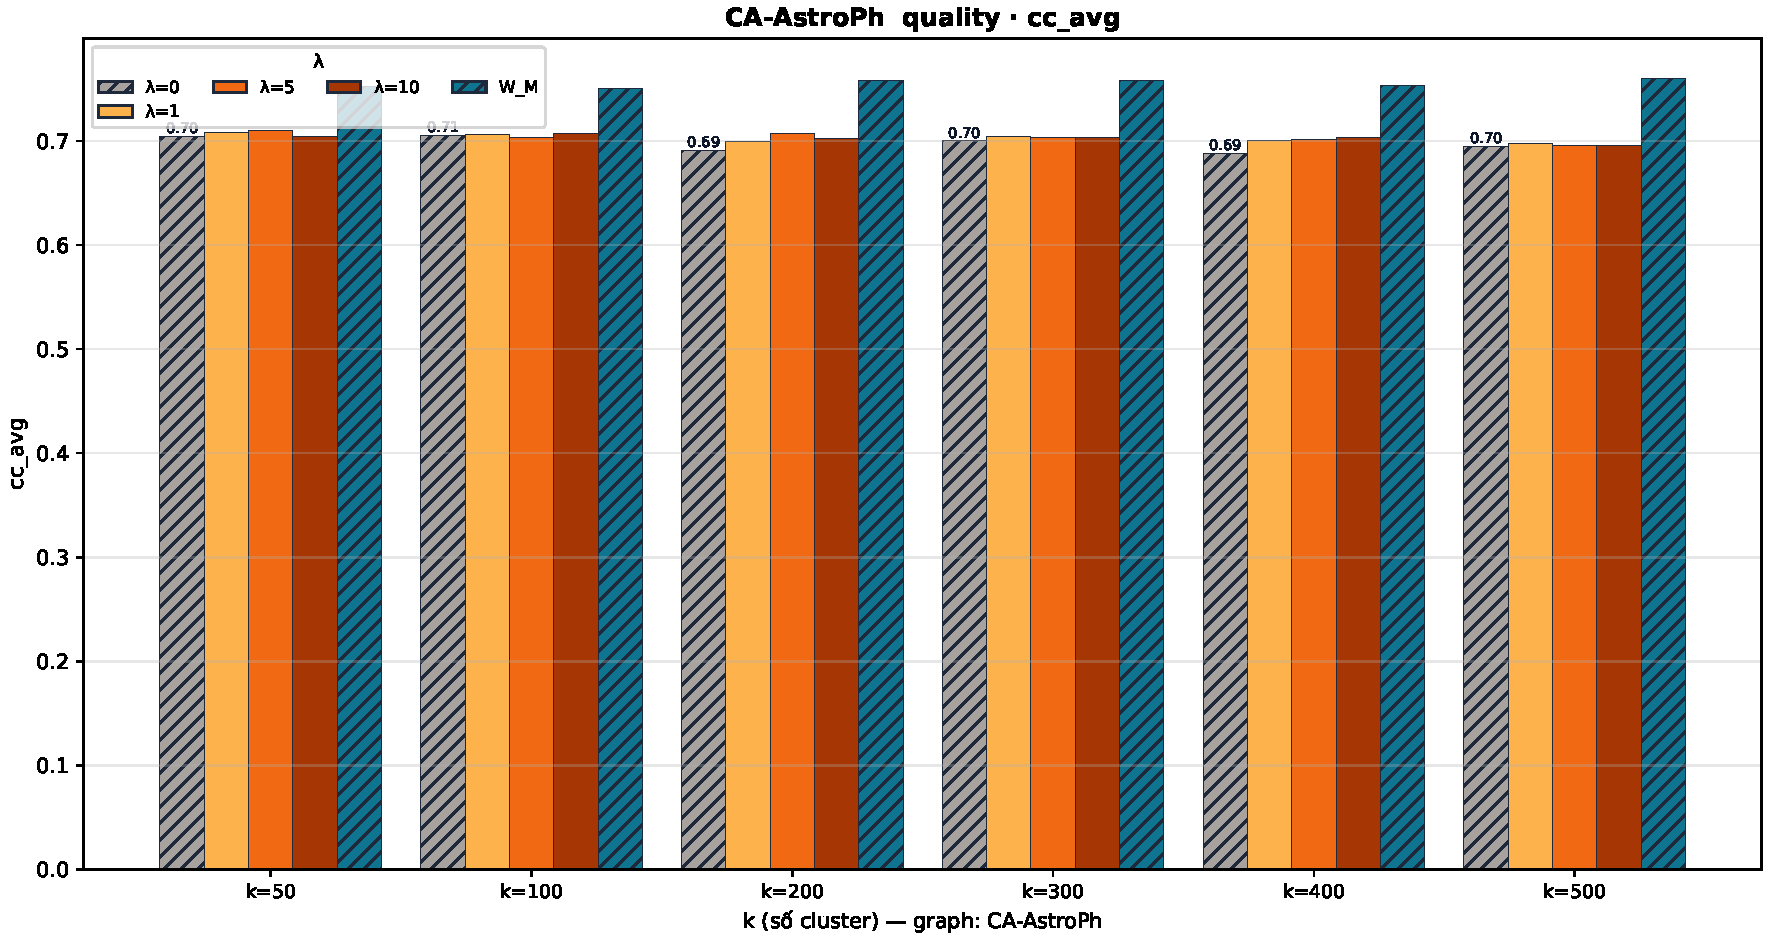
\includegraphics[width=\textwidth]{../main_result/REAL/CA-AstroPh/charts/quality_cc_avg.pdf}
    \caption{$\overline{\mathrm{CC}}$ trên CA-AstroPh theo $\lambda$ và $K$.}
    \label{fig:real-ccavg-astroph}
\end{figure}

Tại $K = 50$, $\overline{\mathrm{CC}}_w(0) = 0{,}6365$ trùng khớp với $cc_{\mathrm{global}}$. $\overline{\mathrm{CC}}_w$ tăng nhẹ lên $0{,}6717$ tại $W_M$. $\overline{\mathrm{CC}}$ bật từ $0{,}7041$ tại $\lambda = 10$ lên $0{,}7518$ tại $W_M$, chênh $0{,}08$ so với $\overline{\mathrm{CC}}_w$. Bứt phá $\overline{\mathrm{CC}}$ tại $W_M$ vừa phải do CA-AstroPh là đồ thị lớn với nhiều nhóm hợp tác có kích thước trung bình, ít cụm cực nhỏ.

\textbf{Kết luận.} CA-AstroPh thuộc nhóm đồ thị đồng tác giả lớn với $cc_{\mathrm{global}}$ cao và phân hoạch ban đầu chất lượng trung bình. Vai trò của $W_\lambda$ chủ yếu là tinh chỉnh modularity, không tạo ra thay đổi cấu trúc tam giác đáng kể.

% ............................................................
\subsection*{CA-CondMat}

Tương tự CA-GrQc nhưng cho lĩnh vực Vật chất ngưng tụ. Hệ số phân cụm toàn cục $cc_{\mathrm{global}} = 0{,}6417$ rất cao, gần với CA-AstroPh.

\textbf{Modularity.}
\begin{figure}[H]
    \centering
    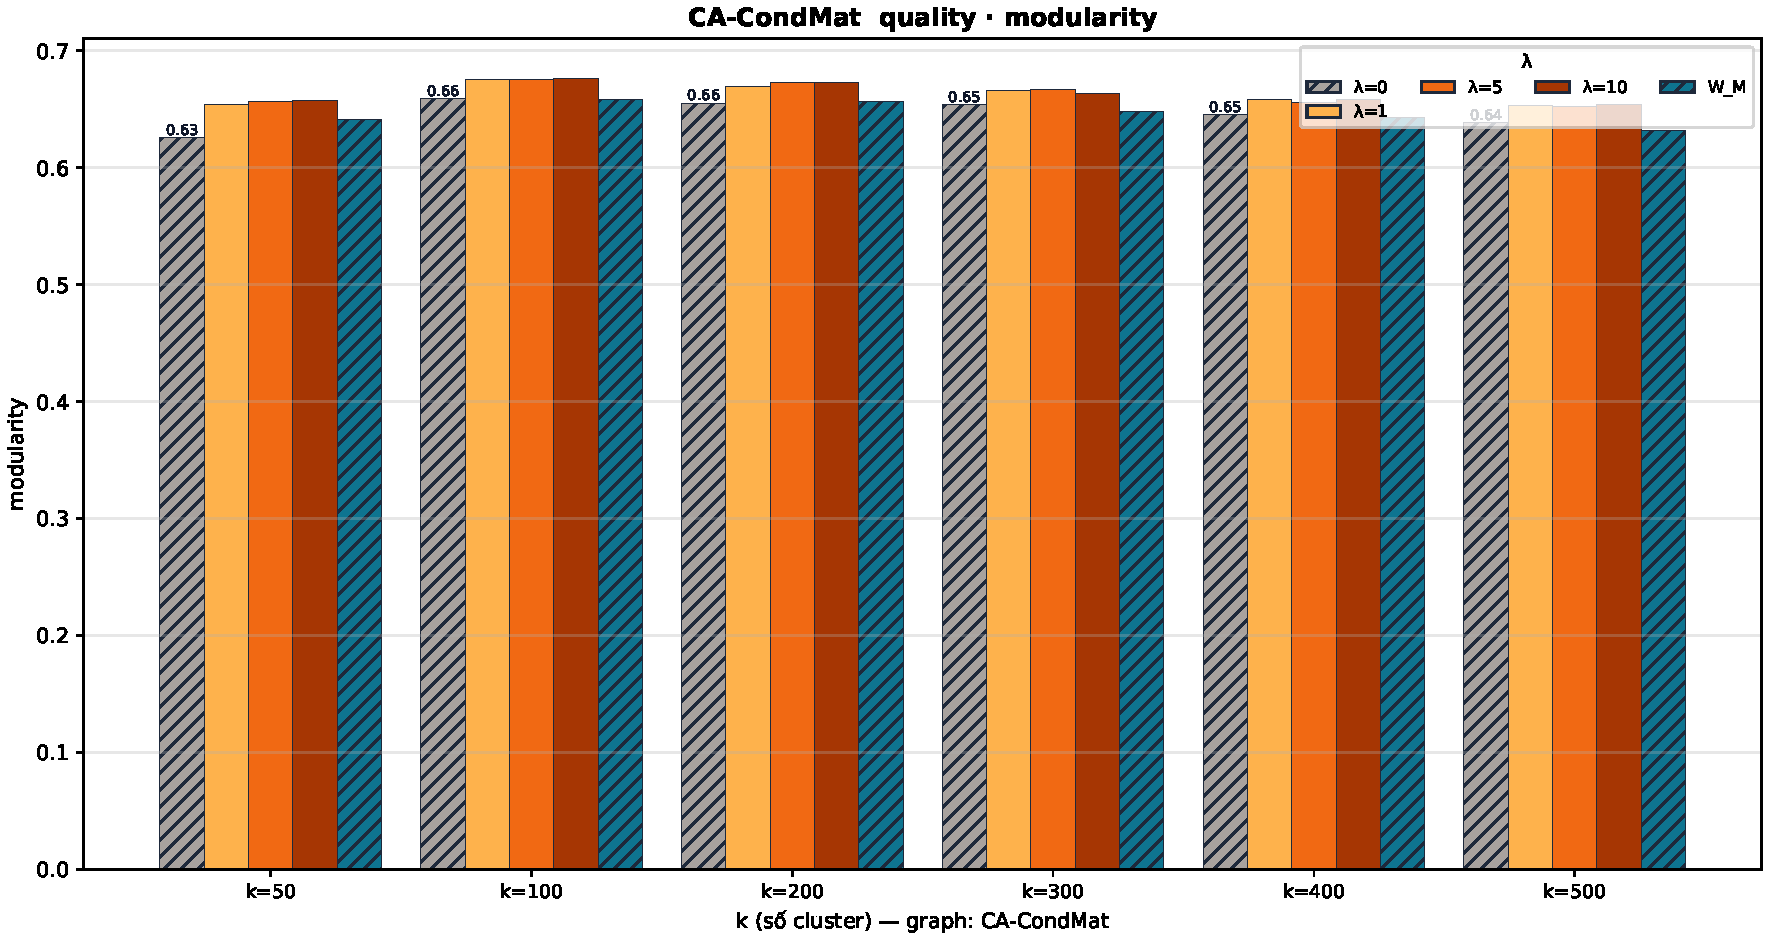
\includegraphics[width=\textwidth]{../main_result/REAL/CA-CondMat/charts/quality_modularity.pdf}
    \caption{Modularity $Q$ trên CA-CondMat theo $\lambda$ và $K$.}
    \label{fig:real-condmat}
\end{figure}

$Q(0)$ cao trên toàn dải ($0{,}62$--$0{,}66$). $\Delta Q$ nhỏ, dao động từ $+0{,}013$ đến $+0{,}032$. Tại $K = 50$, $\Delta Q = +0{,}0316$ với $\lambda^* = 10$. Khi $Q(0)$ đã gần đạt mức cao của thang $Q$, biên độ cải thiện khả dĩ vốn nhỏ nên $\Delta Q$ bị thu hẹp.

\textbf{Hệ số phân cụm.}
\begin{figure}[H]
    \centering
    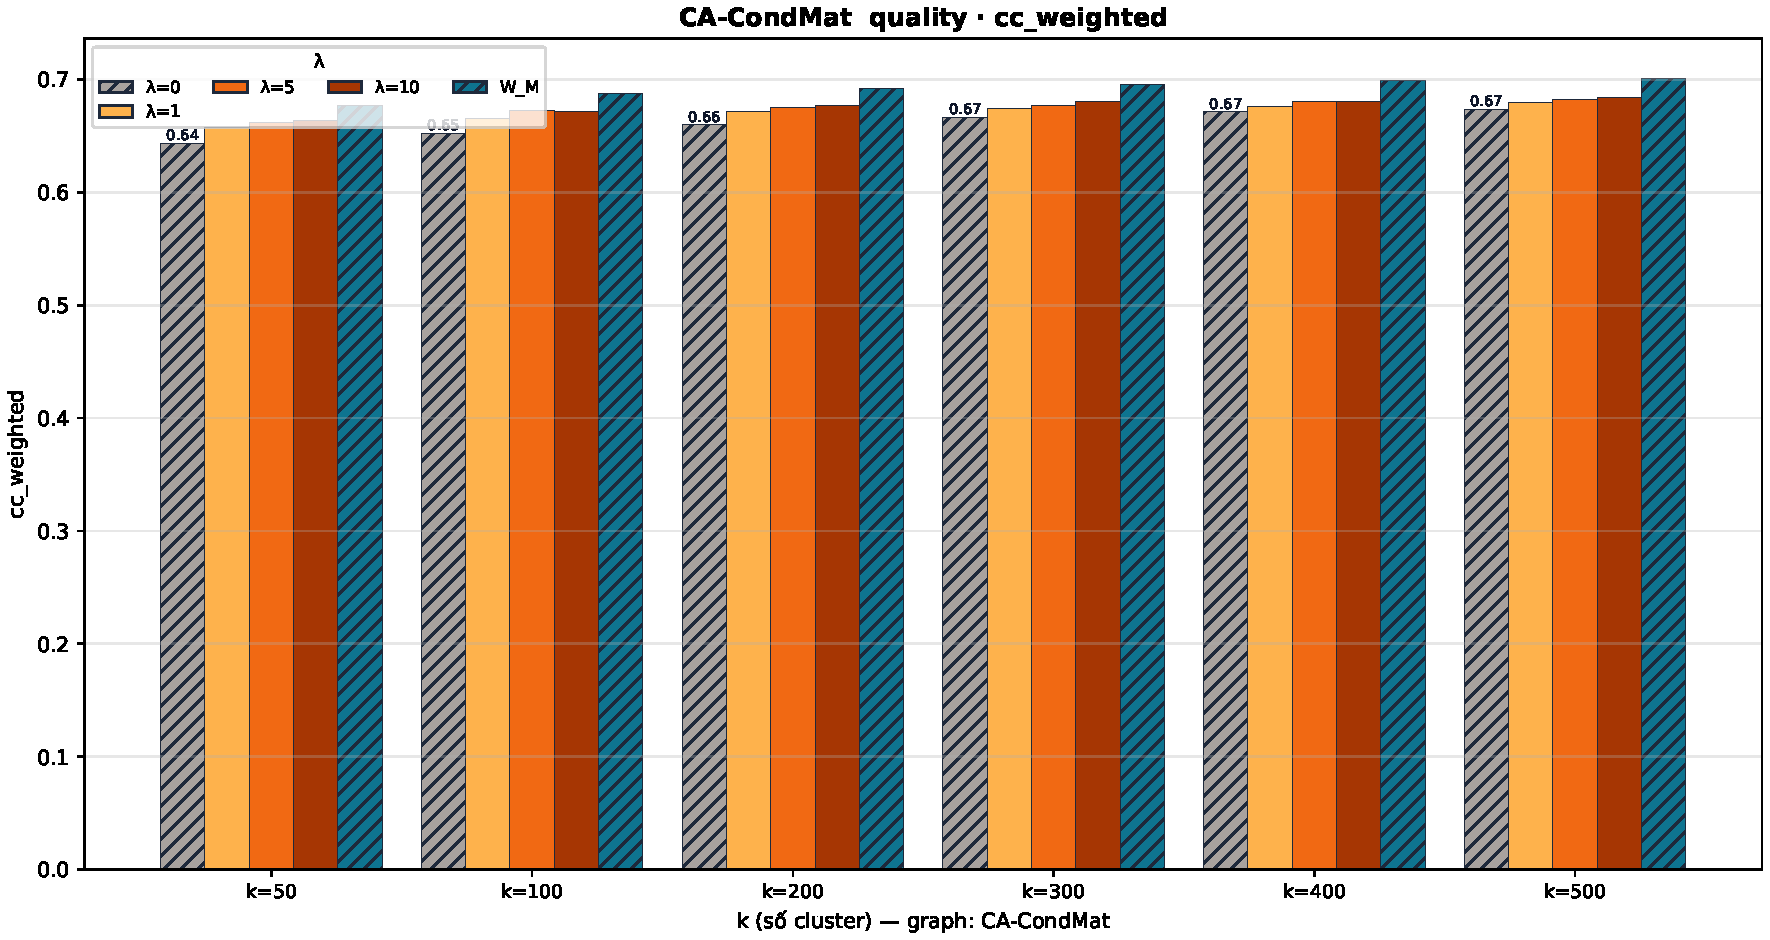
\includegraphics[width=\textwidth]{../main_result/REAL/CA-CondMat/charts/quality_cc_weighted.pdf}
    \caption{$\overline{\mathrm{CC}}_w$ trên CA-CondMat theo $\lambda$ và $K$.}
    \label{fig:real-cc-condmat}
\end{figure}

\begin{figure}[H]
    \centering
    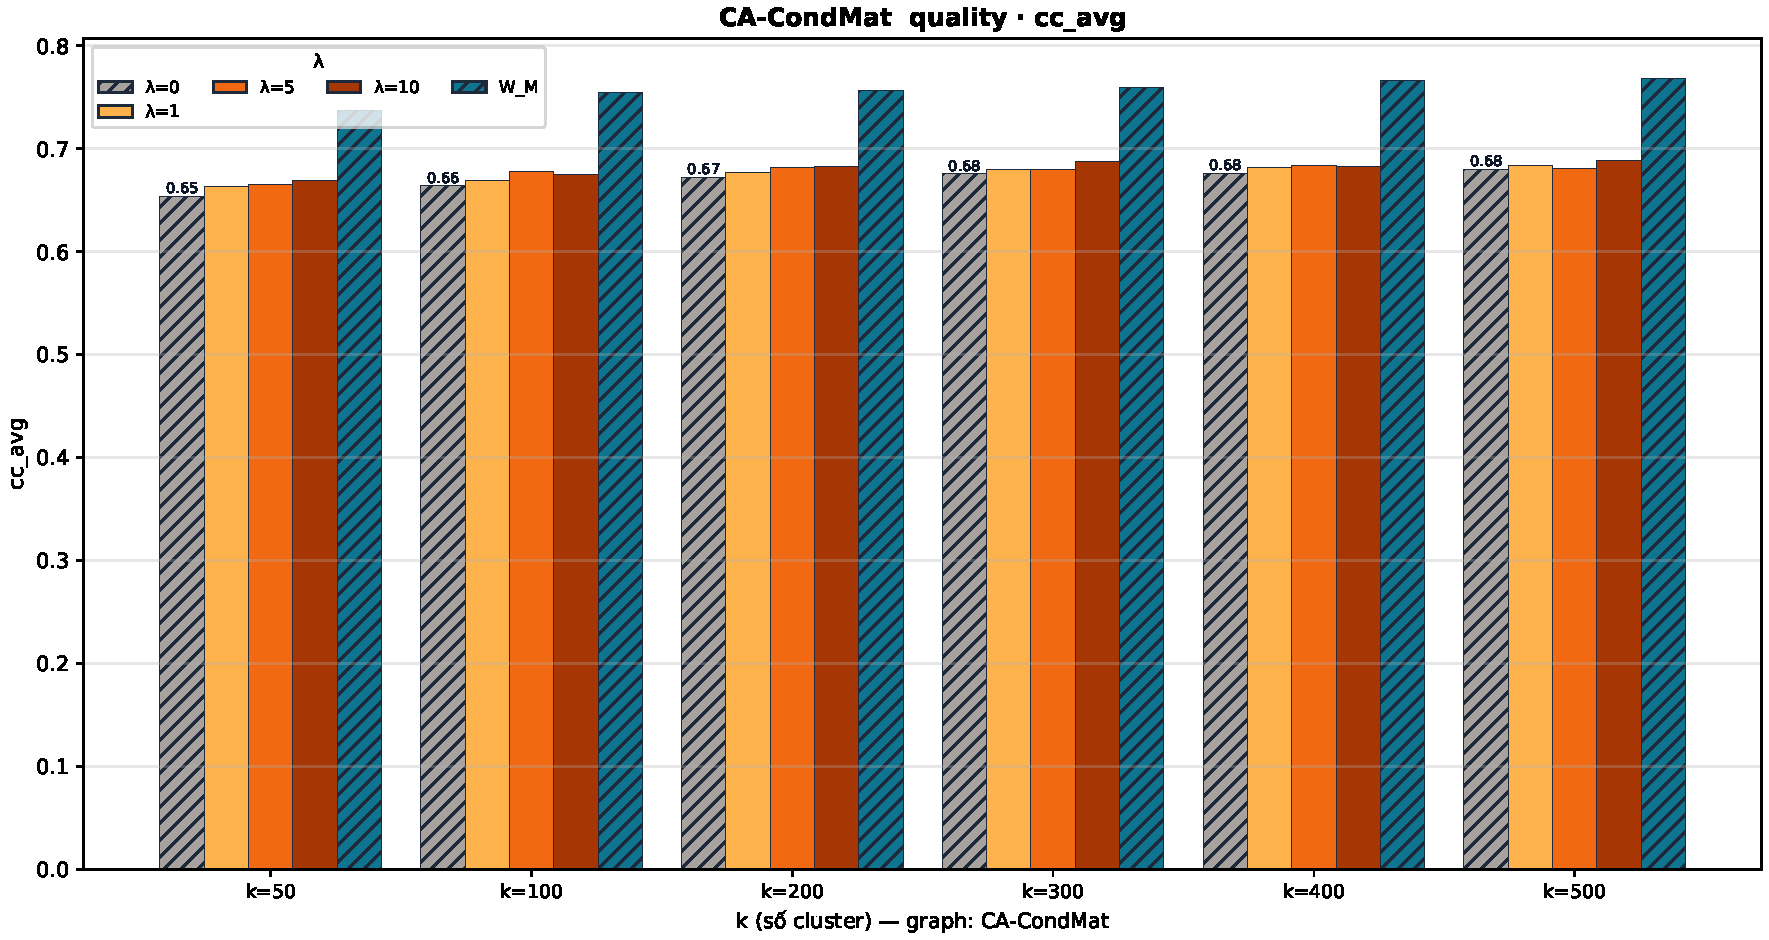
\includegraphics[width=\textwidth]{../main_result/REAL/CA-CondMat/charts/quality_cc_avg.pdf}
    \caption{$\overline{\mathrm{CC}}$ trên CA-CondMat theo $\lambda$ và $K$.}
    \label{fig:real-ccavg-condmat}
\end{figure}

Tại $K = 50$, $\overline{\mathrm{CC}}_w(0) = 0{,}6435$ trùng $cc_{\mathrm{global}}$. Tăng lên $0{,}6769$ tại $W_M$. $\overline{\mathrm{CC}}$ bật từ $0{,}6691$ tại $\lambda = 10$ lên $0{,}7370$ tại $W_M$ (tăng $0{,}07$), trong khi $\overline{\mathrm{CC}}_w$ chỉ tăng $0{,}01$ trong cùng đoạn. Phân mảnh cụm tại $W_M$ ở mức khiêm tốn, $\overline{\mathrm{CC}}_w$ giữ ổn định phản ánh đúng kích thước cụm.

\textbf{Kết luận.} CA-CondMat tái lập pattern của CA-AstroPh và CA-GrQc: mạng đồng tác giả có cấu trúc tam giác mạnh đã được phân cụm phổ trên $A$ khai thác gần tối ưu, $W_\lambda$ chỉ đóng vai trò tinh chỉnh.

% ............................................................
\subsection*{CA-HepTh}

Tương tự CA-GrQc nhưng cho lĩnh vực Vật lý năng lượng cao lý thuyết. Đồ thị đồng tác giả thưa nhất trong nhóm CA-, hệ số phân cụm toàn cục $cc_{\mathrm{global}} = 0{,}4816$ thấp nhất nhóm.

\textbf{Modularity.}
\begin{figure}[H]
    \centering
    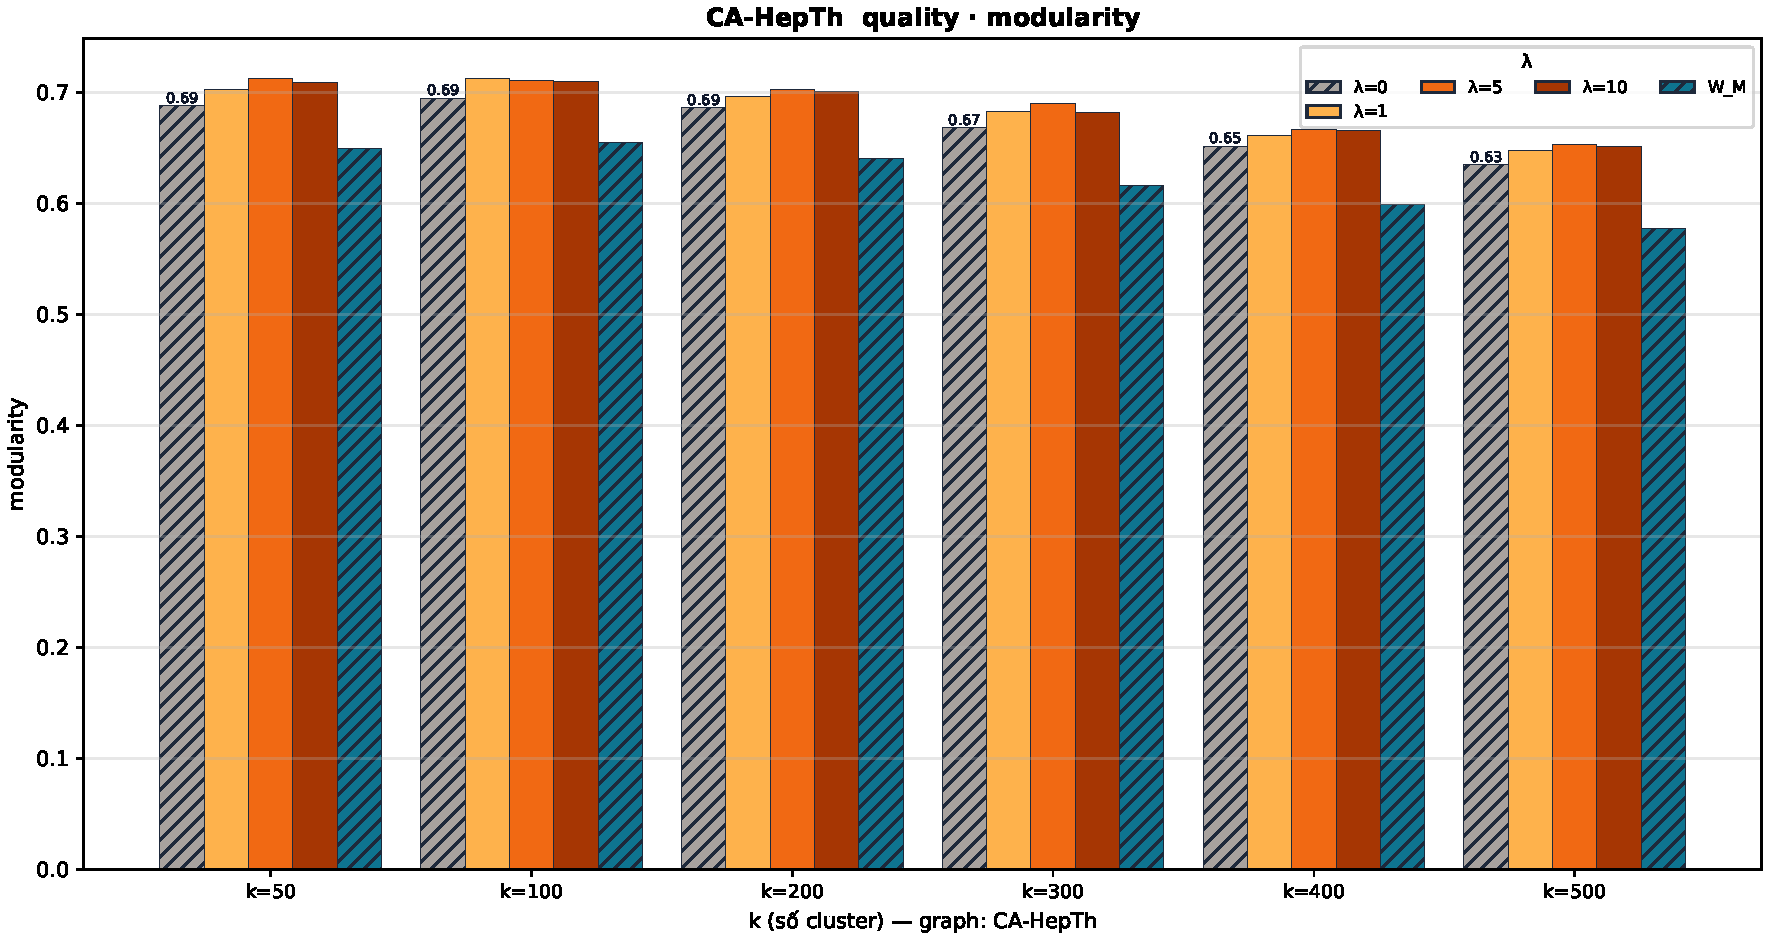
\includegraphics[width=\textwidth]{../main_result/REAL/CA-HepTh/charts/quality_modularity.pdf}
    \caption{Modularity $Q$ trên CA-HepTh theo $\lambda$ và $K$.}
    \label{fig:real-hepth}
\end{figure}

$Q(0)$ cao ($0{,}63$--$0{,}69$). $\Delta Q$ chỉ $+0{,}015$ đến $+0{,}025$, mức cải thiện không đáng kể nhưng đều dương. Tại $K = 50$, $\Delta Q = +0{,}0250$ với $\lambda^* = 5$. Khẳng định thêm xu hướng $\Delta Q$ thu hẹp khi $Q(0)$ đã cao.

\textbf{Hệ số phân cụm.}
\begin{figure}[H]
    \centering
    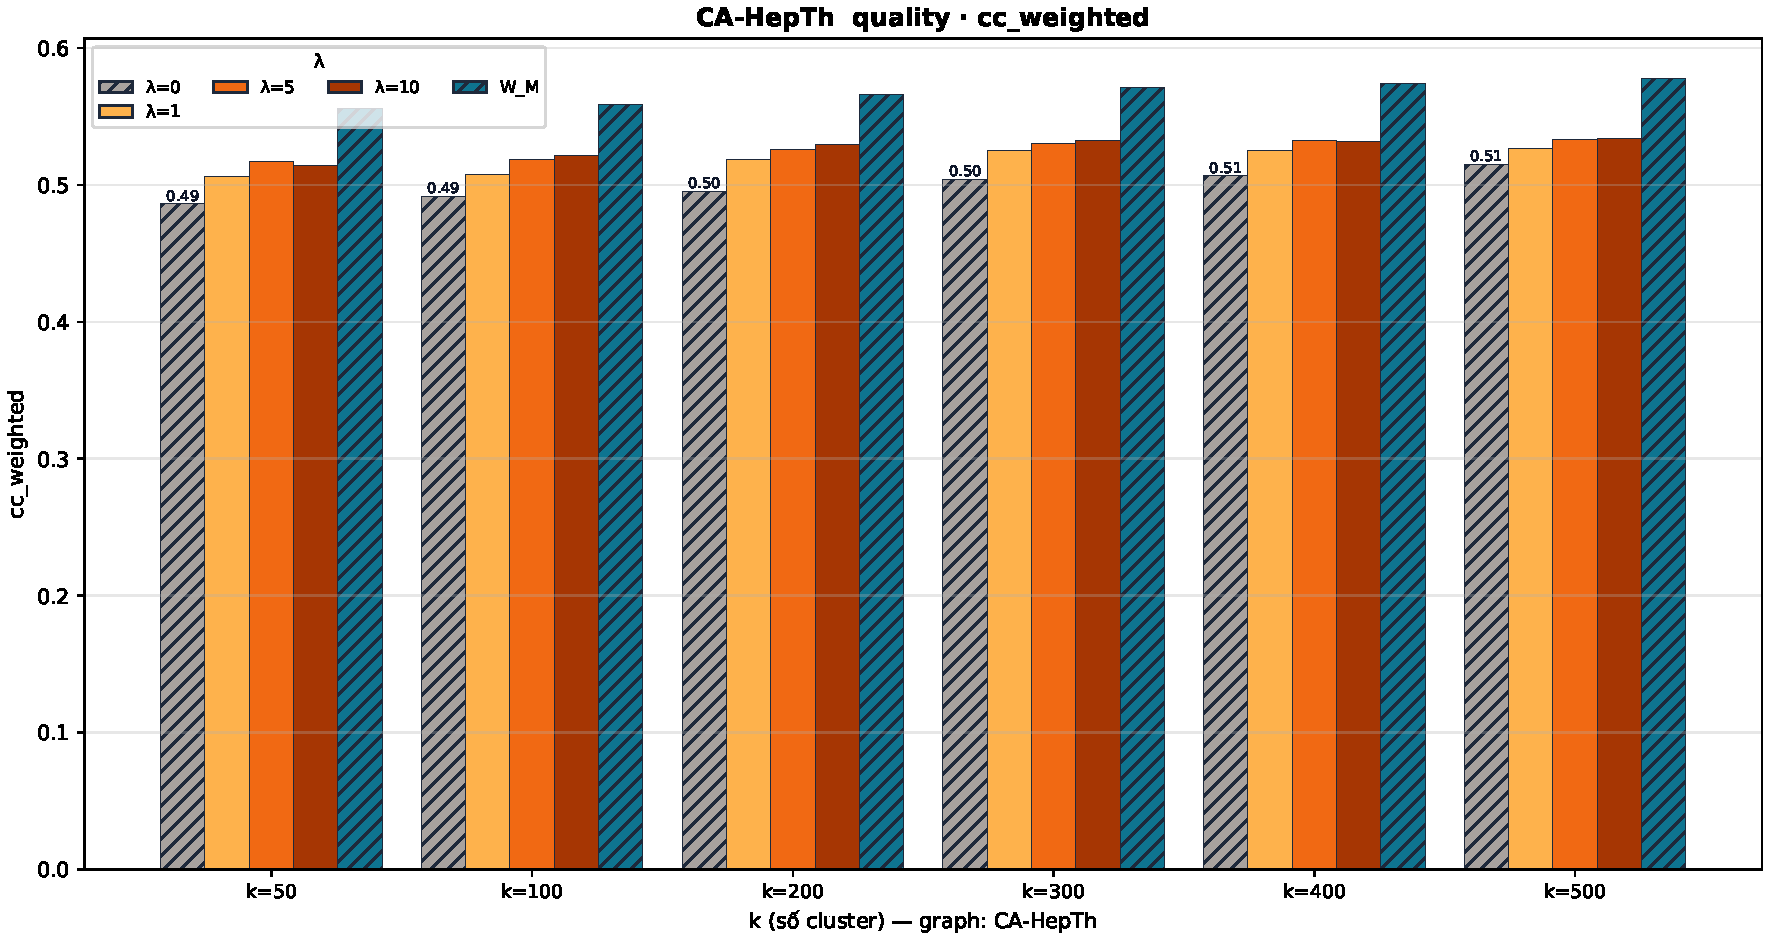
\includegraphics[width=\textwidth]{../main_result/REAL/CA-HepTh/charts/quality_cc_weighted.pdf}
    \caption{$\overline{\mathrm{CC}}_w$ trên CA-HepTh theo $\lambda$ và $K$.}
    \label{fig:real-cc-hepth}
\end{figure}

\begin{figure}[H]
    \centering
    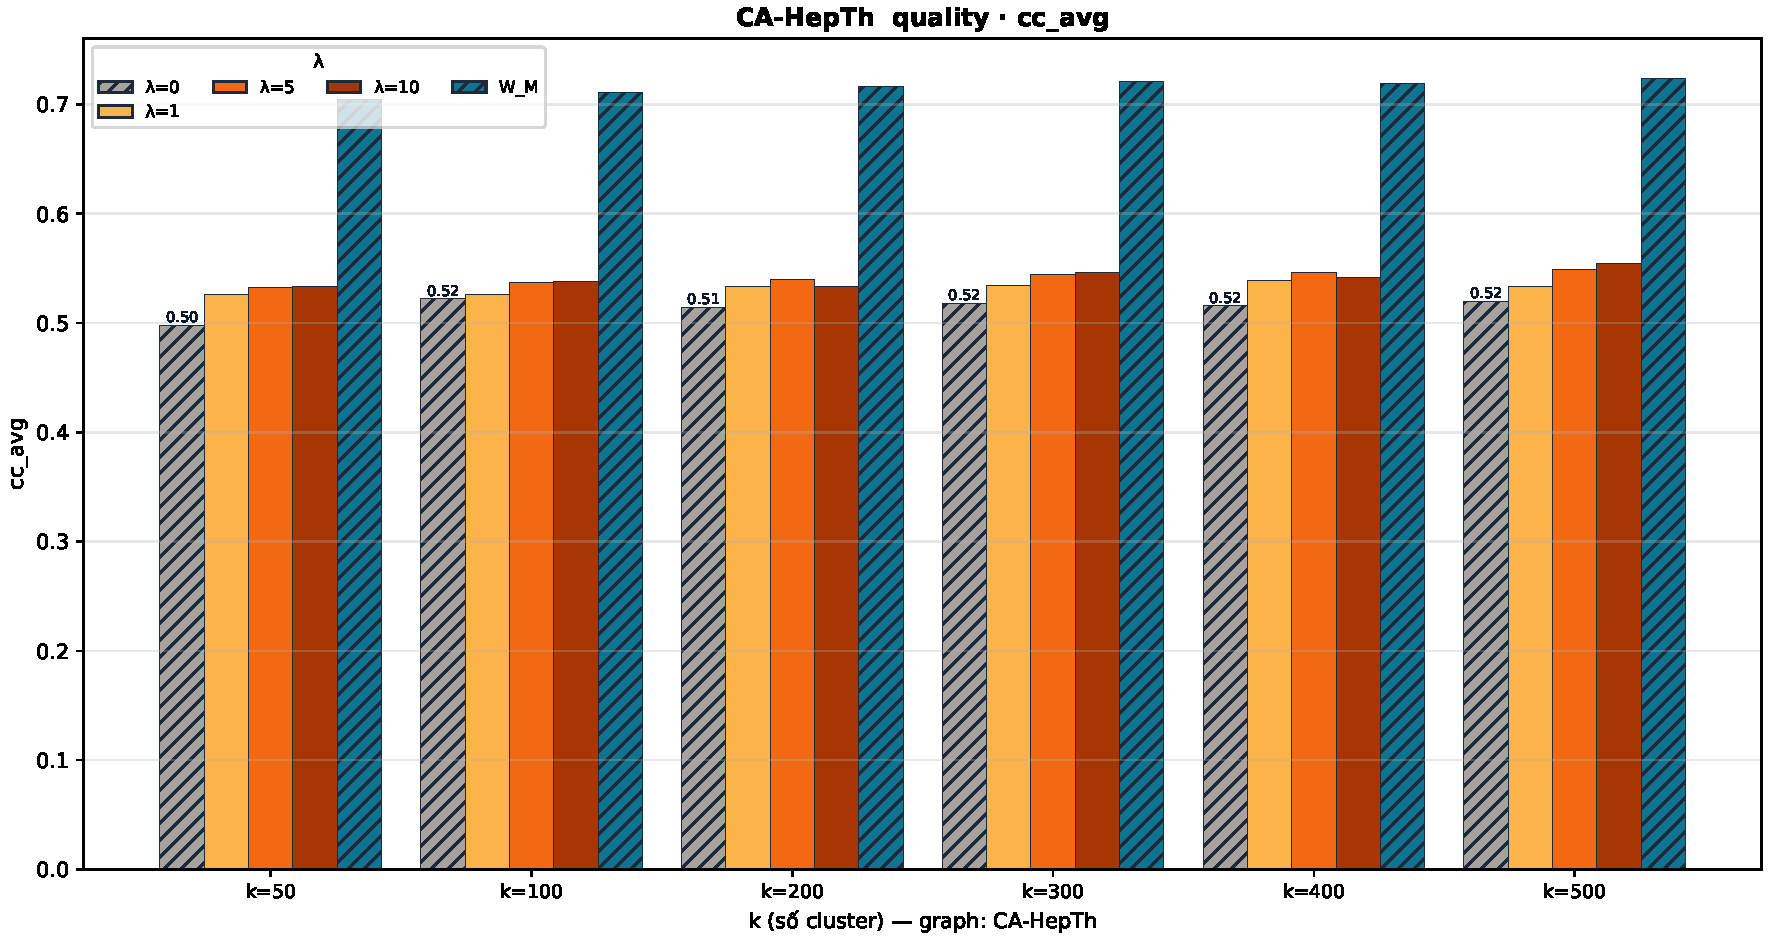
\includegraphics[width=\textwidth]{../main_result/REAL/CA-HepTh/charts/quality_cc_avg.pdf}
    \caption{$\overline{\mathrm{CC}}$ trên CA-HepTh theo $\lambda$ và $K$.}
    \label{fig:real-ccavg-hepth}
\end{figure}

Tại $K = 50$, $\overline{\mathrm{CC}}_w(0) = 0{,}4863$ sát $cc_{\mathrm{global}}$, tăng lên $0{,}5557$ tại $W_M$. $\overline{\mathrm{CC}}$ bật từ $0{,}5337$ tại $\lambda = 10$ lên $0{,}7043$ tại $W_M$, tăng $0{,}17$ chỉ qua một bước trong khi $\overline{\mathrm{CC}}_w$ trong cùng đoạn tăng $0{,}04$. Chênh lệch $0{,}15$ giữa hai đại lượng tại $W_M$ là một trong những chênh lớn nhất trong tập dữ liệu thật, dấu hiệu CA-HepTh có nhiều nhóm nghiên cứu thưa cỡ nhỏ bị $W_M$ tách rời.

\textbf{Kết luận.} CA-HepTh là phiên bản thưa của họ CA-, modularity sớm đạt mức cao nên biên độ cải thiện theo $Q$ nhỏ, nhưng $\overline{\mathrm{CC}}_w$ vẫn có khoảng cải thiện đáng kể. Chênh lớn giữa $\overline{\mathrm{CC}}$ và $\overline{\mathrm{CC}}_w$ phản ánh nhiều nhóm nghiên cứu nhỏ với hệ số phân cụm gần $1$.

% ............................................................
\subsection*{musae\_facebook}

Đỉnh là một trang Facebook công khai, cạnh nối hai trang có liên kết ``like'' lẫn nhau. Cộng đồng phản ánh chủ đề hoặc lĩnh vực của trang. Hệ số phân cụm toàn cục $cc_{\mathrm{global}} = 0{,}3597$, thấp hơn các mạng xã hội cá nhân do quan hệ ``like'' giữa trang phản ánh chủ đề hơn là cộng tác ba bên.

\textbf{Modularity.}
\begin{figure}[H]
    \centering
    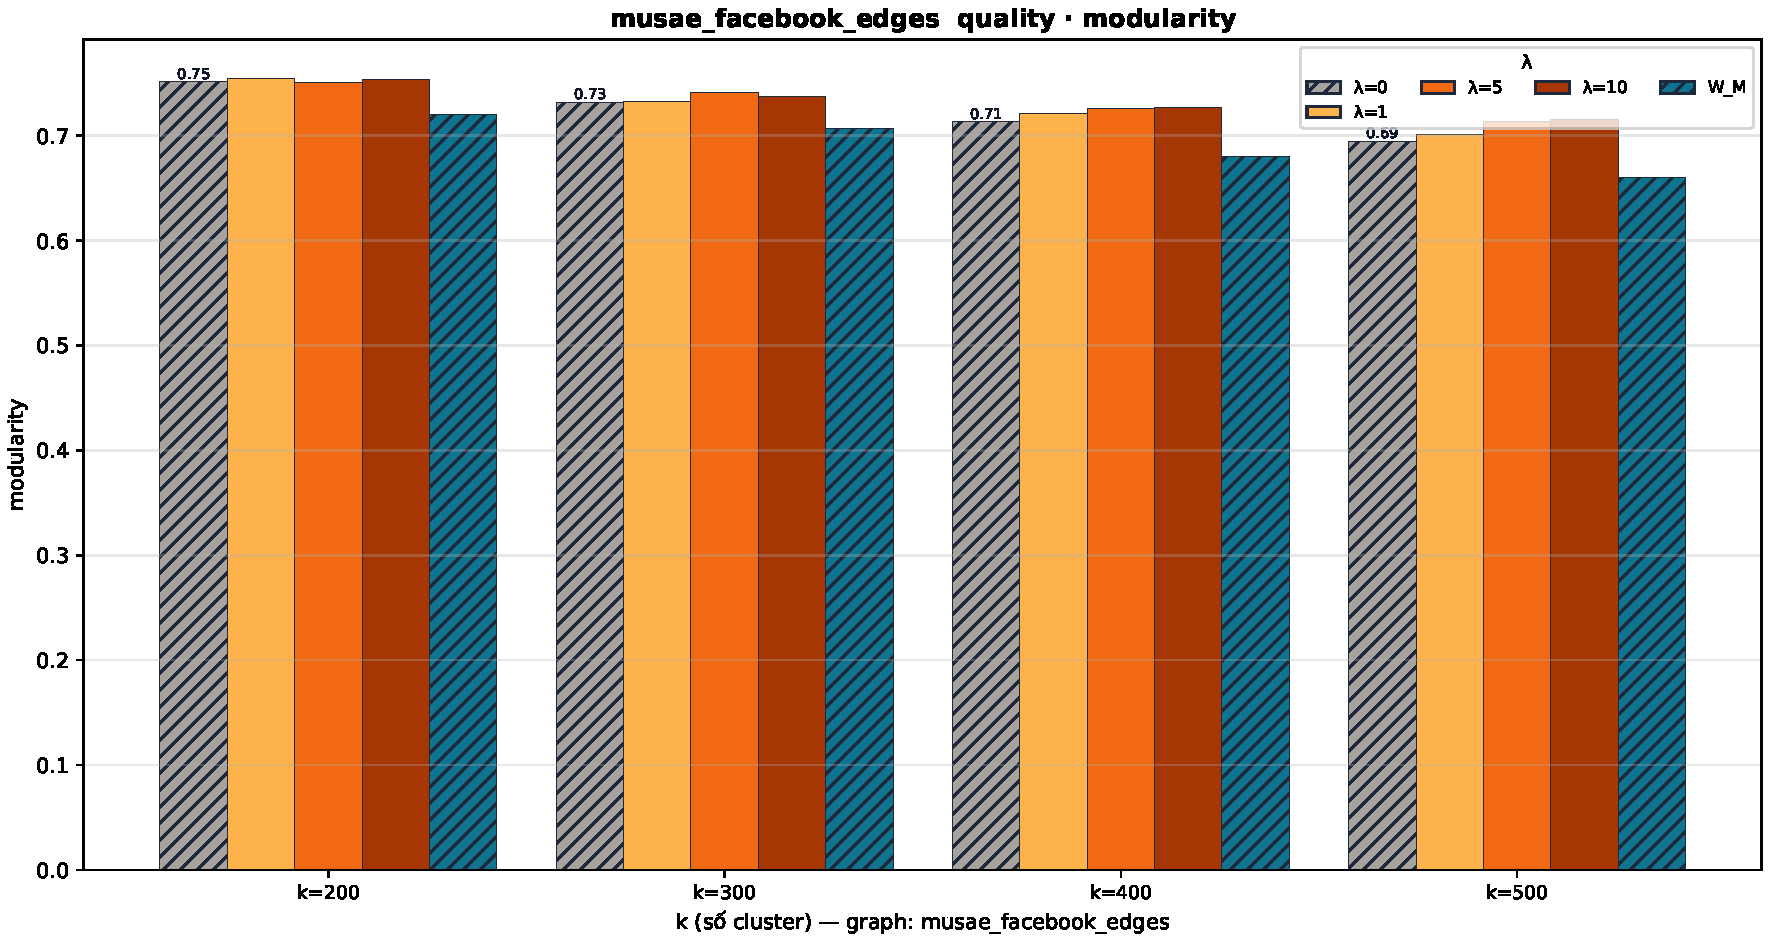
\includegraphics[width=\textwidth]{../main_result/REAL/musae_facebook_edges/charts/quality_modularity.pdf}
    \caption{Modularity $Q$ trên musae\_facebook theo $\lambda$ và $K$.}
    \label{fig:real-musae-fb}
\end{figure}

$Q(0)$ rất cao ($0{,}69$--$0{,}75$). $\Delta Q$ chỉ $+0{,}003$ đến $+0{,}020$, hầu như không thay đổi kết quả phân cụm. Tại $K = 500$, $\Delta Q = +0{,}0202$ với $\lambda^* = 10$. Đây là minh chứng rõ nhất cho xu hướng $\Delta Q$ thu hẹp khi $Q(0)$ đã cao.

\textbf{Hệ số phân cụm.}
\begin{figure}[H]
    \centering
    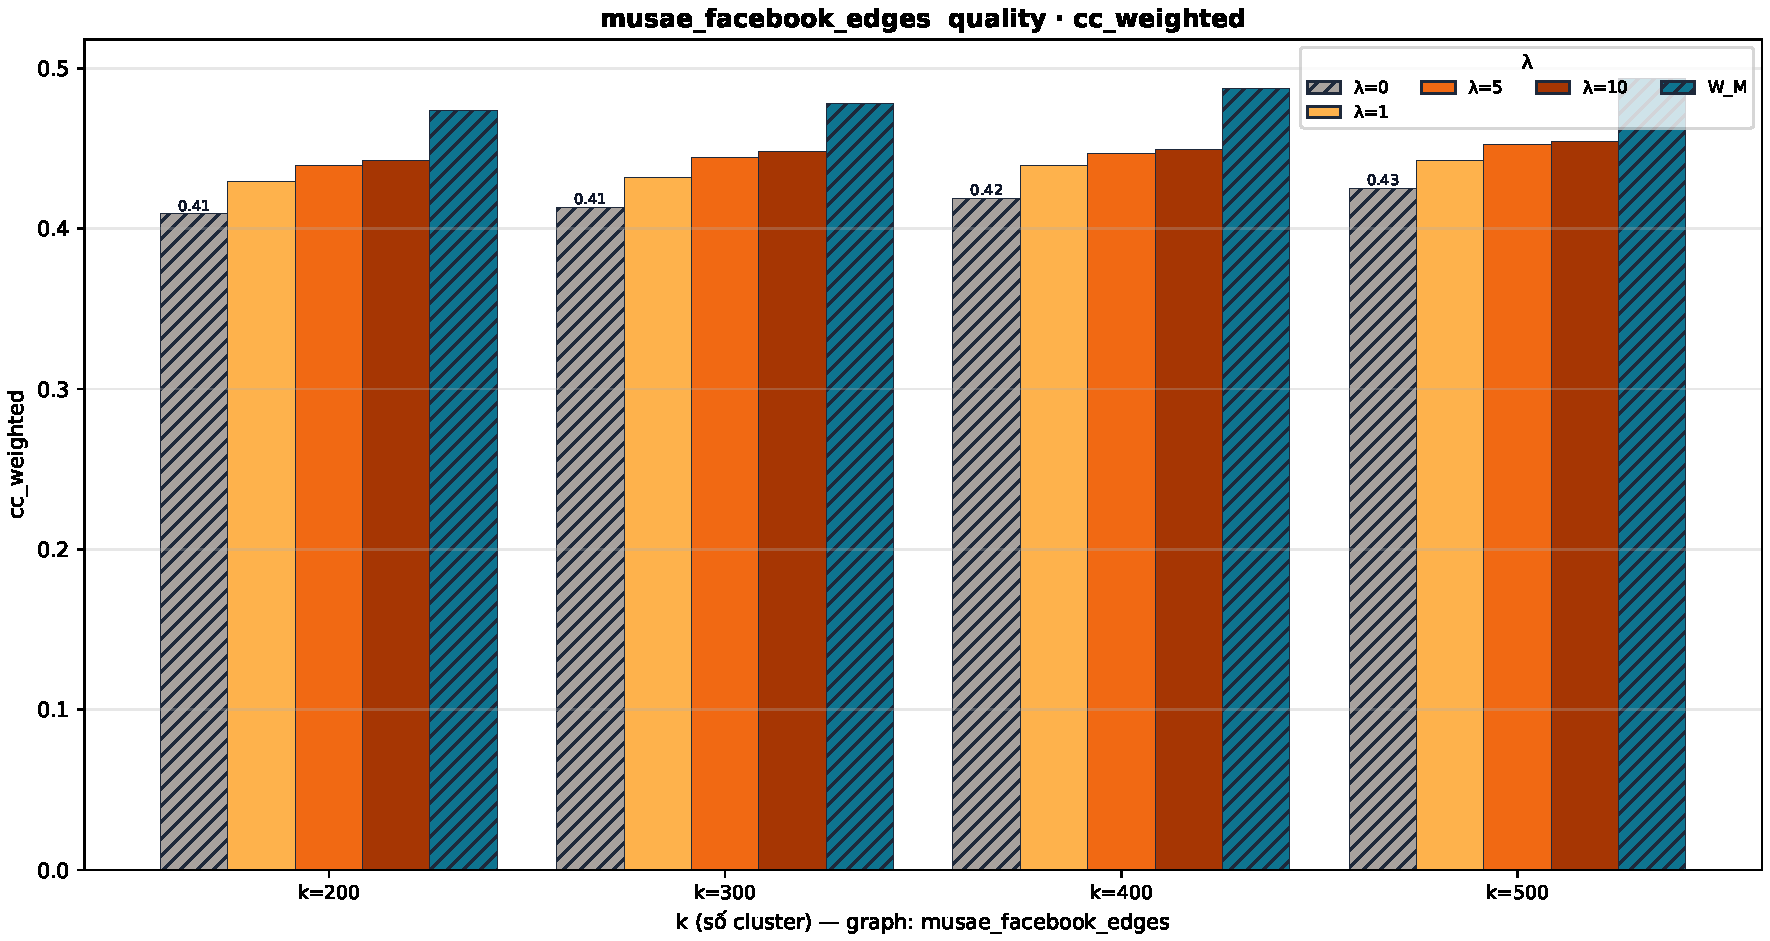
\includegraphics[width=\textwidth]{../main_result/REAL/musae_facebook_edges/charts/quality_cc_weighted.pdf}
    \caption{$\overline{\mathrm{CC}}_w$ trên musae\_facebook theo $\lambda$ và $K$.}
    \label{fig:real-cc-musae-fb}
\end{figure}

\begin{figure}[H]
    \centering
    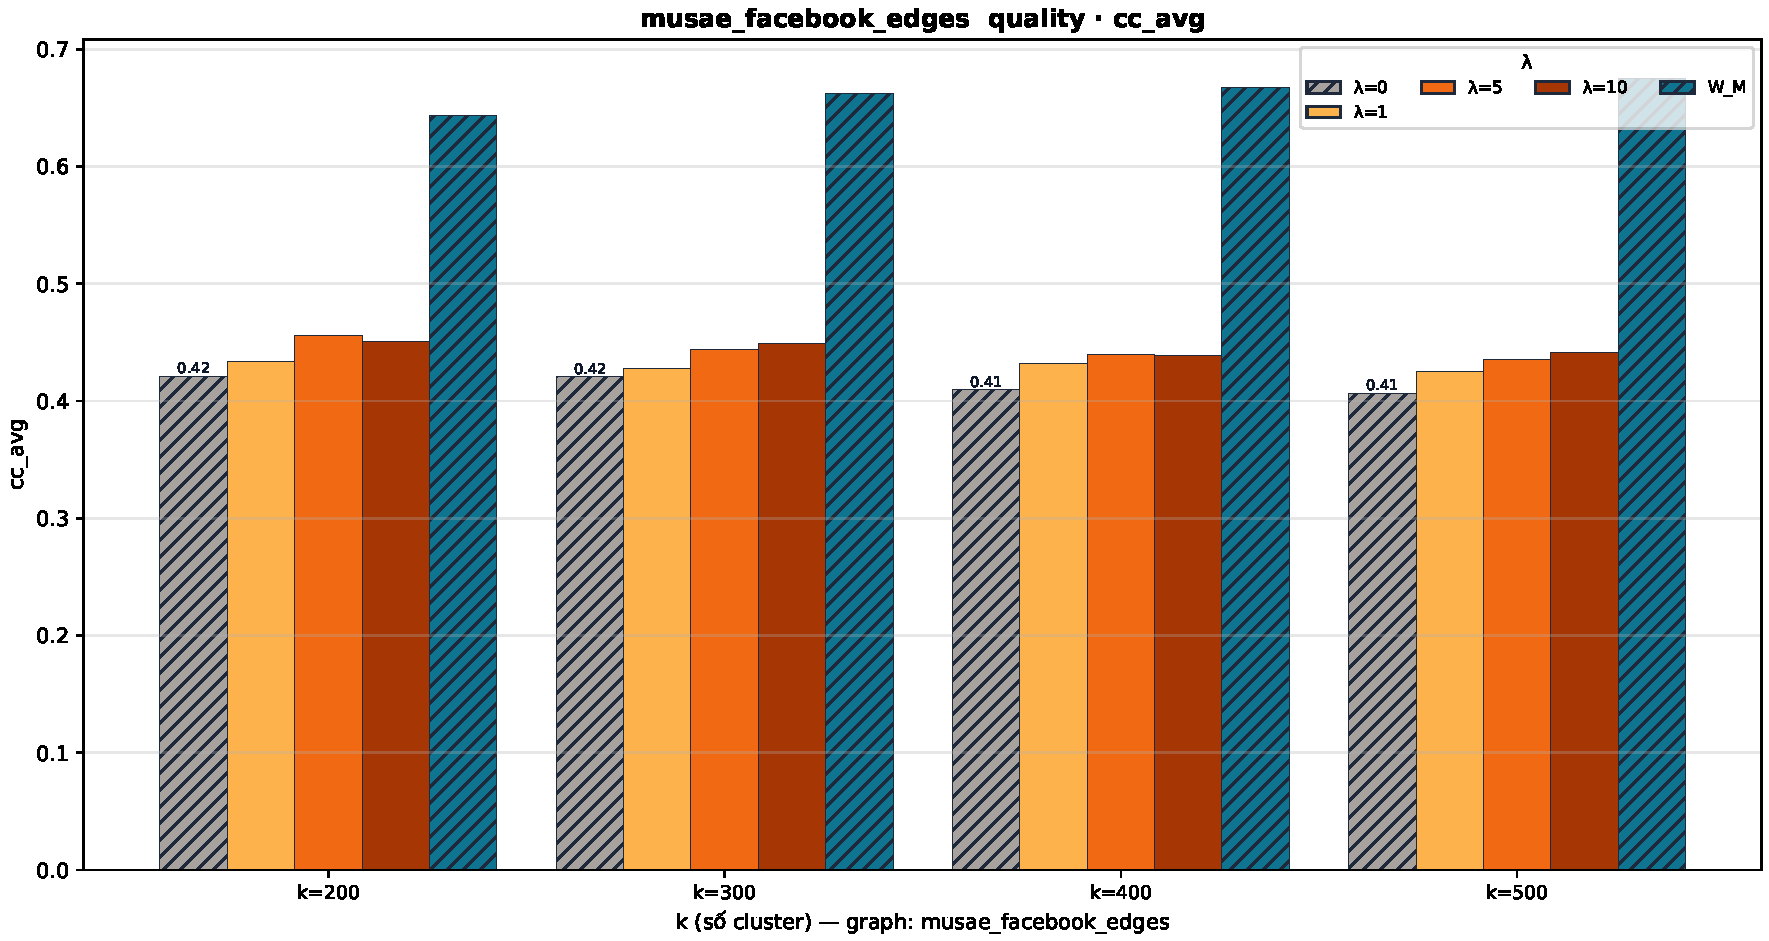
\includegraphics[width=\textwidth]{../main_result/REAL/musae_facebook_edges/charts/quality_cc_avg.pdf}
    \caption{$\overline{\mathrm{CC}}$ trên musae\_facebook theo $\lambda$ và $K$.}
    \label{fig:real-ccavg-musae-fb}
\end{figure}

Tại $K = 200$, $\overline{\mathrm{CC}}_w(0) = 0{,}4091$ đã vượt $cc_{\mathrm{global}}$, dấu hiệu phân cụm phổ trên $A$ đặt được tam giác có sẵn vào trong cụm. $\overline{\mathrm{CC}}_w$ tăng lên $0{,}4737$ tại $W_M$. $\overline{\mathrm{CC}}$ bật từ $0{,}4508$ tại $\lambda = 10$ lên $0{,}6439$ tại $W_M$, tăng $0{,}19$ trong khi $\overline{\mathrm{CC}}_w$ trong cùng đoạn tăng $0{,}03$. Chênh $0{,}17$ giữa hai đại lượng tại $W_M$ phản ánh nhiều chủ đề ngách nhỏ bị tách rời, khẳng định $\overline{\mathrm{CC}}_w$ là chỉ số phù hợp hơn.

\textbf{Kết luận.} musae\_facebook khác biệt với họ musae Twitch ở chỗ quan hệ giữa các trang chủ đề mang tính phân loại hơn là quan hệ xã hội ba bên. Modularity ban đầu đã cao nhờ cấu trúc chủ đề rõ ràng, trọng số motif chỉ tạo ra cải thiện cận biên. Chênh lớn giữa $\overline{\mathrm{CC}}$ và $\overline{\mathrm{CC}}_w$ phản ánh nhiều cụm nhỏ ứng với các chủ đề ngách.

\textbf{Quan sát chung.} Trên cả mười đồ thị, mức cải thiện $\Delta Q$ tỉ lệ nghịch với $Q(0)$, thể hiện hai chế độ rõ rệt:
\begin{itemize}
    \item Khi $Q(0)$ thấp (musae\_DE, musae\_ES, các phân hoạch $K$ lớn của lastfm\_asia và facebook\_combined), ma trận hỗn hợp cải thiện rõ rệt, $\Delta Q$ tới $+0{,}08$ -- $+0{,}12$.
    \item Khi $Q(0)$ đã cao (CA-CondMat, CA-HepTh, musae\_facebook, các phân hoạch $K$ nhỏ của CA-GrQc và facebook\_combined), $\Delta Q$ chỉ $+0{,}001$ -- $+0{,}03$, hầu như không thay đổi kết quả phân cụm.
\end{itemize}
$\Delta Q$ luôn dương trên cả mười đồ thị, nên ma trận hỗn hợp không bao giờ làm giảm chất lượng. Giá trị $\lambda^*$ tối ưu nằm trong khoảng $\{5,\ 10,\ W_M\}$ ở chín trên mười đồ thị, lớn hơn hẳn so với đồ thị sinh ngẫu nhiên ở Mục~\ref{sec:results-synthetic} (chủ yếu là $0{,}5$). Hai đồ thị mạng Twitch (musae\_DE và musae\_ES) cho $\Delta Q$ cao nhất với $\lambda^* \in \{W_M, 1\}$, là dấu hiệu của triadic closure mạnh nhất trong tập dữ liệu.

\textbf{Xác nhận thực nghiệm về vai trò của $\overline{\mathrm{CC}}_w$.} Khoảng cách quan sát được giữa $\overline{\mathrm{CC}}$ và $\overline{\mathrm{CC}}_w$ trên đồ thị thật xác nhận động cơ thiết kế đã trình bày ở Định nghĩa~\ref{def:cc-cluster}. Tại $K = 50$ trên lastfm\_asia, $\overline{\mathrm{CC}}(\lambda^\dagger) = 0{,}6044$ trong khi $\overline{\mathrm{CC}}_w(\lambda^\dagger) = 0{,}3146$, chênh tới $0{,}29$; trên CA-GrQc chênh $0{,}14$; trên CA-HepTh chênh $0{,}15$. Chênh lệch tích cực này hoàn toàn do các cụm rất nhỏ với hệ số phân cụm gần $1$ kéo $\overline{\mathrm{CC}}$ lên cao, dù chúng đóng góp ít vào tổng số đỉnh được phân cụm. Do đó trên dữ liệu thật, $\overline{\mathrm{CC}}$ có xu hướng đánh giá quá lạc quan; $\overline{\mathrm{CC}}_w$ cho con số thận trọng hơn và phản ánh đúng chất lượng phân hoạch.

So sánh giữa các giá trị $\lambda$ cung cấp thêm một bằng chứng thiết kế quan trọng. Trên hầu hết đồ thị thật, $\overline{\mathrm{CC}}$ ở $\lambda = W_M$ bật lên rất cao so với các $\lambda$ hữu hạn — chẳng hạn trên lastfm\_asia tại $K = 50$, $\overline{\mathrm{CC}}$ chuyển từ $0{,}2681$ ở $\lambda = 10$ lên $0{,}6044$ ở $W_M$, gấp hơn hai lần; trên CA-HepTh chuyển từ $0{,}5337$ lên $0{,}7043$; trên musae\_facebook chuyển từ $0{,}4508$ lên $0{,}6439$. Cùng phân hoạch đó, $\overline{\mathrm{CC}}_w$ chỉ tăng nhẹ giữa $\lambda$ hữu hạn và $W_M$, giữ ổn định trong cùng dải biến thiên. Sự bất đối xứng này có lời giải thích trực tiếp: bỏ hoàn toàn ma trận kề $A$ và chỉ dùng $W^{(M)}$ khiến phân cụm phổ tách đồ thị thành nhiều cụm rất nhỏ, vì các đỉnh không nằm trong tam giác trở thành cô lập trong $G_M$ (Mệnh đề~\ref{prop:wlambda-fixes-gm}). Các cụm nhỏ này có hệ số phân cụm cục bộ gần $1$ và đẩy $\overline{\mathrm{CC}}$ lên rất nhanh, nhưng $\overline{\mathrm{CC}}_w$ không bị thổi phồng vì trọng số tỉ lệ với kích thước cụm. Vì vậy mức tăng đo bởi $\overline{\mathrm{CC}}_w$ phản ánh đúng phần đóng góp thực của motif vào chất lượng phân hoạch; $\overline{\mathrm{CC}}$ thì bị ảnh hưởng nặng bởi hiện tượng phân mảnh cụm khi $\lambda \to \infty$.

% ============================================================
\section{Tổng hợp: hai chế độ tối ưu của $\lambda$}
\label{sec:summary-results}

Kết hợp toàn bộ kết quả thực nghiệm, $\lambda^*$ tối ưu thể hiện hai chế độ trái ngược, phụ thuộc vào cơ chế sinh cạnh của đồ thị.

\begin{table}[H]
\centering
\caption{Hai chế độ tối ưu của $\lambda^*$ phụ thuộc loại đồ thị}
\label{tab:two-regimes}
\begin{tabular}{|>{\arraybackslash}p{4cm}|>{\arraybackslash}p{3.5cm}|>{\arraybackslash}p{6cm}|}
\hline
\textbf{Loại đồ thị} & $\lambda^*$ quan sát & \textbf{Cơ chế sinh tam giác} \\ \hline
SBM, Planted, GRPG & $0{,}5$ -- $1$ & Tam giác là hệ quả thống kê của mật độ cạnh, không độc lập với cạnh. \\ \hline
LFR khó ($\mu \geq 0{,}35$) & $0{,}5$ -- $5$ & Tam giác cũng từ cấu hình cạnh, nhưng phân bố bậc power-law tạo các vùng tam giác đậm đặc cục bộ. \\ \hline
Mạng xã hội thật & $5$ -- $W_M$ & Triadic closure tạo tam giác có chủ đích, mang tín hiệu cộng đồng độc lập với cạnh đơn lẻ. \\ \hline
\end{tabular}
\end{table}

Quan sát then chốt: $\lambda^*$ phụ thuộc \emph{tỷ lệ tín hiệu cộng đồng giữa tam giác và cạnh}. Khi tam giác chỉ là hệ quả thống kê của cạnh (các mô hình ngẫu nhiên), thêm trọng số motif nhiều làm pha loãng cạnh và giảm chất lượng phân hoạch, do đó $\lambda^*$ nhỏ. Khi tam giác mang tín hiệu cấu trúc riêng vượt xa kỳ vọng độc lập (mạng xã hội thật), trọng số motif lớn lại có lợi và $\lambda^*$ dịch về phía $W_M$. Đây là biểu hiện thực nghiệm của Nhận xét~\ref{rem:random-triangle} ở Phụ lục~\ref{appx:random-models}.

\textbf{Kết quả tổng quát.} Ma trận hỗn hợp $W_\lambda$ với $\lambda^*$ chọn phù hợp luôn cho modularity tốt hơn hoặc bằng $A$ thuần trên cả $35$ bộ test sinh ngẫu nhiên và các cấu hình $(K)$ trên mười đồ thị thật. Trên các bộ test khó nhất, mức cải thiện $\Delta Q$ vượt $+0{,}1$. Điều này xác nhận giả thiết lý thuyết ở Chương~\ref{chap:thuat-toan}: việc gộp thông tin cạnh và motif qua một tham số nội suy duy nhất là một mở rộng có giá trị thực nghiệm cho phân cụm phổ.

\cleardoublepage
